\documentclass[a4paper,12pt,openany,titlepage]{scrartcl}
\usepackage[utf8]{inputenc}
\usepackage[T1]{fontenc}
\usepackage[a4paper,left=2cm,right=2cm,top=2.5cm,bottom=2.5cm]{geometry}
\usepackage[french]{babel}
\usepackage{libertine}
\usepackage[pdftex]{graphicx}
\usepackage{booktabs}
\usepackage{array}
\usepackage{tabularx}
\usepackage{float}
\usepackage{amsmath,amssymb}
\usepackage{longtable}
\usepackage{enumitem}
\usepackage{hyperref}
\usepackage[table]{xcolor}
\usepackage{listings}
\usepackage{caption}
\usepackage{subcaption}
\usepackage{tikz}
\usepackage{pgfgantt}
\usepackage{scrlayer-scrpage}

% ============================================================
% DESIGN & COLOR PREFERENCES (SEMESTER REPORT THEME)
% ============================================================
\definecolor{NavyBlue}{RGB}{12, 35, 64}
\definecolor{AccentColor}{RGB}{204, 51, 0}
\definecolor{LightBlue}{RGB}{240, 244, 250}

\addtokomafont{section}{\color{NavyBlue}\sffamily}
\addtokomafont{subsection}{\color{NavyBlue}\sffamily}
\addtokomafont{subsubsection}{\color{NavyBlue}\sffamily}
\setkomafont{captionlabel}{\color{NavyBlue}\sffamily\bfseries}
\setkomafont{caption}{\small}

% ============================================================
% HEADERS & FOOTERS (scrlayer-scrpage)
% ============================================================
\pagestyle{scrheadings}
\clearpairofpagestyles
\ihead{\color{NavyBlue}\sffamily\small PROJET BURNTRACK \textbullet{} GROUPE 7}
\ohead{\color{NavyBlue}\sffamily\small\pagemark}
\cfoot[\pagemark]{} % page numbers centered in footer for plain style (front matter)
\addtokomafont{pagehead}{\normalfont}
\KOMAoptions{headsepline=0.5pt}
\addtokomafont{headsepline}{\color{NavyBlue}}

\setlength{\parindent}{0cm}
\setlength{\parskip}{1ex plus 0.5ex minus 0.2ex}
\newcommand{\hsp}{\hspace{20pt}}
\newcommand{\HRule}{\color{AccentColor}\rule{\linewidth}{0.8mm}\color{black}}

\hypersetup{colorlinks=true,linkcolor=NavyBlue,citecolor=AccentColor,urlcolor=NavyBlue}

\lstset{basicstyle=\ttfamily\small,breaklines=true,frame=single,backgroundcolor=\color{gray!8},keywordstyle=\color{NavyBlue},commentstyle=\color{green!50!black},numbers=left,numberstyle=\tiny\color{gray},xleftmargin=2em}

\linespread{1.4}\selectfont
\begin{document}

% ============================================================
% PAGE DE TITRE
% ============================================================
\begin{titlepage}
  \begin{sffamily}
  \begin{minipage}{0.48\textwidth}
    \begin{flushleft}
      
\includegraphics[height=1.8cm]{CENTRALE_CASA_LOGO_OK.png}
    \end{flushleft}
  \end{minipage}
  \hfill
  \begin{minipage}{0.48\textwidth}
    \begin{flushright}
      
\includegraphics[height=3.2cm]{burntrack_logo_white.png}
    \end{flushright}
  \end{minipage}
  \\[1.5cm]
  
  \begin{center}
    \textsc{\LARGE École Centrale Casablanca}\\[0.8cm]
    \textsc{\LARGE PROJET LEARNING BY DOING}\\[0.4cm]
    \textsc{\large Année universitaire 2025--2026}\\[1.5cm]

    \HRule \\[0.4cm]
    { \huge \bfseries \color{NavyBlue} BurnTrack : Rover Autonome pour la Prédiction de Propagation d'Incendies Forestiers \\[0.4cm] }
    \HRule \\[2.5cm]

    \begin{minipage}[t]{0.48\textwidth}
      \begin{flushleft} \large
        \textbf{\underline{Équipe de Conception :}}\\
        \vfill
        MOUNIR Anwar\\
        AZGRAR Meryem\\
        LATIFI Chady\\
        DIONE Amina\\
        MALEU Ivan Emmanuel Rabe\\
      \end{flushleft}
    \end{minipage}
    \hfill
    \begin{minipage}[t]{0.48\textwidth}
      \begin{flushright} \large
         \textbf{\underline{Sous la supervision de :}}\\
         \vfill
         Pr. BELHBOUB Anouar\\
      \end{flushright}
    \end{minipage}

    \vfill
    {\large Juin 2026}
  \end{center}
  \end{sffamily}
\end{titlepage}

% ============================================================
% DÉDICACES
% ============================================================
\newpage
\pagestyle{empty}
\thispagestyle{empty}
\vspace*{5cm}
\begin{center}
\textit{\large À nos familles, pour leur soutien inconditionnel.}
\end{center}
\newpage

\tableofcontents
\listoffigures
\listoftables
\newpage

% ============================================================
% LISTE DES ACRONYMES
% ============================================================
\section*{Liste des acronymes et abréviations}
\addcontentsline{toc}{section}{Liste des acronymes}

\begin{tabularx}{\textwidth}{lX}
\textbf{CA} & Cellular Automaton (Automate Cellulaire) \\
\textbf{CBOR} & Concise Binary Object Representation \\
\textbf{CFL} & Courant--Friedrichs--Lewy (condition de stabilité) \\
\textbf{CNN} & Convolutional Neural Network \\
\textbf{DFMC} & Dead Fuel Moisture Content \\
\textbf{GPS} & Global Positioning System \\
\textbf{HPUA} & Heat Per Unit Area \\
\textbf{IMU} & Inertial Measurement Unit \\
\textbf{LHMC} & Live Herbaceous Moisture Content \\
\textbf{LoRa} & Long Range (protocole radio basse consommation) \\
\textbf{MAE} & Mean Absolute Error \\
\textbf{MLP} & Multi-Layer Perceptron \\
\textbf{NDVI} & Normalized Difference Vegetation Index \\
\textbf{ONNX} & Open Neural Network Exchange \\
\textbf{PLBD} & Projet Learning By Doing \\
\textbf{PWM} & Pulse Width Modulation \\
\textbf{ROS} & Rate of Spread (vitesse de propagation) \\
\textbf{RPi4} & Raspberry Pi 4 \\
\textbf{SAV} & Surface Area to Volume ratio \\
\textbf{VPD} & Vapour Pressure Deficit \\
\end{tabularx}

\newpage
\pagenumbering{arabic}
\setcounter{page}{1}
\pagestyle{plain}

% ============================================================
% REMERCIEMENTS
% ============================================================
\section{Remerciements}

Nous tenons tout d'abord à exprimer notre profonde gratitude envers notre encadrant, pour son accompagnement tout au long de ce projet. Ses orientations et ses remarques nous ont permis de structurer notre démarche et d'aboutir aux résultats présentés dans ce rapport.

Nous remercions également l'administration de l'École Centrale Casablanca, et en particulier l'équipe du FabLab, pour la mise à disposition des équipements d'impression 3D et de prototypage qui ont été essentiels à la réalisation de la partie matérielle du projet.

Nous tenons également à exprimer une gratitude toute particulière à nos parents, impliqués bien malgré eux à diverses étapes de cette aventure (que ce soit pour le transport logistique des pièces, le soutien lors des séances d'assemblage nocturnes ou le support moral indispensable).

Enfin, nous remercions l'ensemble des membres du groupe pour l'esprit collaboratif qui a animé ce projet tout au long de l'année.

\vspace{0.8cm}

% ============================================================
% RÉSUMÉ & ABSTRACT
% ============================================================
\section{Résumé}

Les incendies de forêt constituent une menace croissante pour les écosystèmes marocains et africains, aggravée par le changement climatique. Les modèles de prédiction existants, calibrés sur la végétation nord-américaine, ne sont pas directement applicables aux biomes africains. Ce projet propose \textbf{BurnTrack}, un système intégré combinant un rover autonome de collecte de données environnementales et une plateforme de simulation de propagation d'incendies.

Le système repose sur quatre piliers : (1) un moteur Rothermel v3 corrigé, implémentant 50 modèles de combustible dont 28 spécifiques à l'Afrique~; (2) un automate cellulaire stochastique couplé à un correcteur par apprentissage automatique (MLP, $R^2 = 0{,}987$, MAE $= 0{,}735$ m/min sur le dataset de littérature de 1\,840 observations terrain)~; (3) un rover 6WD/6WS à base de Raspberry Pi 4, équipé de capteurs environnementaux, d'un anémomètre DIY et d'une caméra pour la classification botanique par vision artificielle (YOLO + CNN)~; (4) une communication LoRa entre le rover et la station de base, couplée à une visualisation en temps réel par WebSocket.

La navigation autonome du rover utilise l'algorithme D* Lite pour planifier des trajectoires en évitant le front de feu, avec re-planification dynamique. Les résultats montrent une amélioration significative de la prédiction du taux de propagation par rapport au modèle Rothermel brut.

\vspace{0.8cm}

\section{Abstract}

Forest fires constitute an escalating threat to Moroccan and African ecosystems, worsened by climate change. Existing prediction models, calibrated on North American vegetation, are not directly applicable to African biomes. This project introduces \textbf{BurnTrack}, an integrated system combining an autonomous environmental data collection rover and a fire propagation simulation platform.

The system relies on four pillars: (1) a corrected Rothermel v3 engine, implementing 50 fuel models including 28 specific to Africa; (2) a stochastic cellular automaton coupled with a machine learning corrector (MLP, $R^2 = 0.987$, MAE $= 0.735$ m/min on the literature dataset of 1,840 field observations); (3) a Raspberry Pi 4-based 6WD/6WS rover, equipped with environmental sensors, a DIY anemometer, and a camera for botanical classification via computer vision (YOLO + CNN); (4) a LoRa communication link between the rover and the base station, coupled with real-time WebSocket visualization.

The autonomous navigation of the rover utilizes the D* Lite algorithm to plan paths avoiding the fire front, with dynamic replanning. The results demonstrate a significant improvement in rate of spread prediction compared to the raw Rothermel model, paving the way for proactive fire management.

\newpage
\pagestyle{scrheadings}

% ============================================================
% INTRODUCTION
% ============================================================
\section{Introduction}

Les incendies de forêt représentent un enjeu environnemental majeur à l'échelle mondiale. Au Maroc, la forêt couvre environ 9 millions d'hectares --- soit 12\,\% du territoire national --- et subit chaque année des pertes considérables. Selon le Haut Commissariat aux Eaux et Forêts et à la Lutte Contre la Désertification, plus de 10\,000 hectares sont ravagés annuellement, principalement dans les régions du Rif, du Moyen Atlas et de la Maâmora. Le changement climatique, en allongeant les saisons sèches et en intensifiant les vagues de chaleur, aggrave cette situation de manière alarmante.

Face à ce constat, la prédiction du comportement des feux de forêt s'avère essentielle pour une gestion proactive des risques. Le modèle semi-empirique de Rothermel (1972), qui constitue la référence mondiale en matière de modélisation de la propagation de surface, présente néanmoins deux limites fondamentales dans le contexte africain~: premièrement, ses modèles de combustible standard (BEHAVE) ont été calibrés sur la végétation nord-américaine~; deuxièmement, les données d'observation terrain nécessaires à sa calibration sont quasi inexistantes pour les écosystèmes africains.

Notre projet, \textbf{BurnTrack}, vise à combler ce double déficit en proposant une approche intégrée articulée autour de deux axes complémentaires~:

\begin{itemize}[nosep]
    \item \textbf{Un axe simulation} : adaptation du modèle de Rothermel avec 28 modèles de combustible spécifiques aux écosystèmes marocains et africains, couplage avec un automate cellulaire stochastique, et correction par apprentissage automatique à partir de données de la littérature scientifique.
    \item \textbf{Un axe robotique} : conception et réalisation d'un rover autonome 6WD/6WS capable de collecter des données environnementales \textit{in situ} (température, humidité, vent, pente, qualité de l'air) et d'identifier les espèces végétales par vision artificielle, alimentant ainsi le modèle de simulation en boucle fermée.
\end{itemize}

Ce rapport présente les travaux réalisés au cours de l'année universitaire 2025--2026. Après une présentation du contexte et de la problématique (section~4), nous détaillons l'état de l'art des modèles de feu et des rovers de surveillance (section~4.3). Nous décrivons ensuite l'architecture technique de la solution (section~4.4), les détails de réalisation et les tests effectués (section~4.5), puis les résultats obtenus et leur analyse (section~4.6). Nous concluons par les perspectives d'amélioration et de déploiement terrain.

\vspace{0.8cm}

% ============================================================
% DÉVELOPPEMENT DU PROJET
% ============================================================
\section{Développement du projet}

% ------------------------------------------------------------
\subsection{Planification et Répartition des Rôles}

Le projet s'est déroulé sur les deux semestres de l'année universitaire 2025--2026, selon le découpage temporel présenté dans le tableau~\ref{tab:phases} et le diagramme de Gantt (figure~\ref{fig:gantt}).

\begin{table}[H]
\centering
\caption{Phases clés du projet BurnTrack}
\label{tab:phases}
\begin{tabularx}{\textwidth}{|l|l|X|}
\hline
\rowcolor{NavyBlue} \textcolor{white}{\textbf{Phase}} & \textcolor{white}{\textbf{Période}} & \textcolor{white}{\textbf{Activités principales}} \\
\hline
Cadrage & Sep--Nov 2025 & Cahier des charges, étude bibliographique, choix technologiques \\
\hline
Conception & Déc 2025--Fév 2026 & Conception mécanique (CAO), modélisation 3D, commande matériel, architecture logicielle \\
\hline
Prototypage & Fév--Mar 2026 & Impression 3D (13 pièces), assemblage châssis, câblage initial, tests moteurs \\
\hline
Développement & Mar--Mai 2026 & Moteur Rothermel v3, modèles de combustible, pipeline vision, premiers correcteurs ML \\
\hline
Intégration & Mai--Juin 2026 & Automate cellulaire, navigation D* Lite, protocole LoRa, visualisation WebSocket, tests d'intégration \\
\hline
Finalisation & Juin 2026 & Calibration, rédaction du rapport, préparation de la soutenance \\
\hline
\end{tabularx}
\end{table}

\begin{figure}[H]
\centering
\begin{ganttchart}[
    hgrid,
    vgrid,
    x unit=0.58cm,
    y unit title=0.6cm,
    y unit chart=0.7cm,
    title height=1,
    bar/.style={fill=blue!40},
    bar height=0.5,
    group right shift=0,
    group top shift=0.1,
    group height=.2,
    group peaks width=0.2,
    milestone/.style={fill=red, draw=red, shape=ganttmilestone}
]{1}{20}
\gantttitle{2025--2026}{20} \\
\gantttitlelist{9,10,11,12,1,2,3,4,5,6}{2} \\
\ganttgroup{Cadrage \& Biblio}{1}{4} \\
\ganttbar{Cahier des charges}{1}{2} \\
\ganttbar{Étude bibliographique}{2}{4} \\
\ganttgroup{Conception}{5}{8} \\
\ganttbar{Conception CAO Châssis}{5}{7} \\
\ganttbar{Architecture logicielle}{6}{8} \\
\ganttgroup{Prototypage}{9}{12} \\
\ganttbar{Impression 3D}{9}{11} \\
\ganttbar{Câblage \& Drivers}{10}{12} \\
\ganttgroup{Développement}{13}{16} \\
\ganttbar{Moteur Rothermel v3}{13}{15} \\
\ganttbar{Pipeline Vision ONNX}{14}{16} \\
\ganttgroup{Intégration \& Tests}{17}{20} \\
\ganttbar{Automate Cellulaire}{17}{18} \\
\ganttbar{Couplage \& D* Lite}{18}{19} \\
\ganttbar{Calibration \& Rapport}{19}{20}
\end{ganttchart}
\caption{Diagramme de Gantt du projet BurnTrack}
\label{fig:gantt}
\end{figure}

L'organisation interne de l'équipe a été structurée de manière à exploiter les compétences spécifiques de chaque membre, tout en assurant des phases d'intégration collaborative~:

\begin{itemize}
    \item \textbf{MOUNIR Anwar} (Simulation \& Machine Learning) :
        \begin{itemize}[nosep]
            \item Réécriture et correction du moteur Rothermel v3 en Python.
            \item Développement du correcteur MLP par réseau de neurones et calibration des hyperparamètres.
            \item Implémentation du planificateur de chemin dynamique D* Lite et de l'algorithme Dijkstra multi-sources.
            \item Développement de la plateforme de visualisation WebSocket/Flask.
        \end{itemize}
    \item \textbf{AZGRAR Meryem} (Conception Mécanique \& Impression 3D) :
        \begin{itemize}[nosep]
            \item Modélisation CAO du châssis WildWilly sous SolidWorks.
            \item Optimisation des pièces structurelles pour impression 3D (PLA) et gestion de l'impression au FabLab.
            \item Conception mécanique du système de suspension rocker-bogie et montage mécanique du châssis.
        \end{itemize}
    \item \textbf{LATIFI Chady} (Électronique \& Firmware Embarqué) :
        \begin{itemize}[nosep]
            \item Choix des composants matériels et routage du schéma de câblage sous Fritzing.
            \item Configuration de l'environnement matériel (Raspberry Pi 4, PCA9685, ADS1015, capteurs).
            \item Programmation des drivers bas niveau pour le contrôle des moteurs DC et servos de direction.
            \item Implémentation de la logique de contrôle cinématique 6WS/6WD.
        \end{itemize}
    \item \textbf{DIONE Amina} (Vision Artificielle \& Télédétection) :
        \begin{itemize}[nosep]
            \item Entraînement et optimisation du modèle de classification botanique (YOLO) et de sécheresse (CNN).
            \item Export et intégration du pipeline de vision sous format ONNX Runtime pour exécution sur le RPi4.
            \item Collecte des données de télédétection et liaison avec les modèles de combustible.
        \end{itemize}
    \item \textbf{MALEU Ivan Emmanuel Rabe} (Système de Communication \& Protocole IoT) :
        \begin{itemize}[nosep]
            \item Conception du protocole LoRa et définition des formats d'encodage CBOR compacts.
            \item Programmation de la passerelle de communication ESP32 LoRa et liaison série USB.
            \item Gestion de la fiabilité de la transmission radio (mécanismes d'acquittement et retries).
        \end{itemize}
\end{itemize}

% ------------------------------------------------------------
\subsection{Contexte et problématique}

\subsubsection{Le risque incendie au Maroc}

Le Maroc est particulièrement vulnérable aux feux de forêt en raison de sa position géographique, de son climat méditerranéen à semi-aride et de la diversité de ses écosystèmes forestiers. Les principales zones à risque comprennent~:

\begin{itemize}[nosep]
    \item La forêt de la Maâmora (130\,000 ha au total, dont environ 73\,000 ha de chêne-liège)
    \item Les cédraies du Moyen Atlas (\textit{Cedrus atlantica})
    \item Le maquis méditerranéen du Rif
    \item L'arganeraie du Souss (\textit{Argania spinosa}, endémique)
    \item La forêt de Bouskoura (périurbaine, 2\,800 ha) --- notre cas d'étude
\end{itemize}

La forêt de Bouskoura, située à 12 km au sud de Casablanca (33,535°N, 7,645°W), présente un intérêt particulier en raison de sa proximité urbaine et des risques que représenterait un incendie non maîtrisé pour les zones résidentielles environnantes.

\subsubsection{Limites des modèles existants}

Le modèle de Rothermel, bien que référence mondiale, souffre de deux limitations majeures dans le contexte africain~:

\begin{enumerate}[nosep]
    \item \textbf{Absence de modèles de combustible africains}~: les modèles standard BEHAVE de la littérature (comprenant les 13 modèles historiques d'Anderson (1982) et les 40 modèles de Scott \& Burgan (2005)) décrivent la végétation nord-américaine. Les propriétés physico-chimiques de la végétation africaine (chaleur de combustion, rapport surface/volume, charge de combustible) diffèrent significativement.
    \item \textbf{Manque de données d'observation}~: les études publiées sur le comportement du feu en Afrique sont rares (environ 1\,840 observations exploitables, issues de 7 études sur 30 ans), contre des dizaines de milliers pour l'Amérique du Nord.
\end{enumerate}

\subsubsection{Objectifs du projet}

Face à ces constats, BurnTrack poursuit les objectifs suivants~:

\begin{enumerate}[nosep]
    \item Développer des modèles de combustible calibrés pour les écosystèmes marocains et africains
    \item Implémenter un moteur Rothermel corrigé, couplé à un automate cellulaire et un correcteur par apprentissage automatique
    \item Concevoir un rover autonome capable de collecter les données environnementales nécessaires à la calibration du modèle
    \item Établir un protocole de communication IoT pour la transmission en temps réel des données terrain
    \item Développer une plateforme de visualisation interactive des cartes de risque
\end{enumerate}

% ------------------------------------------------------------
\subsection{État de l'art}

\subsubsection{Modèles de propagation des feux de surface}

\paragraph{Le modèle de Rothermel (1972).} Le modèle semi-empirique de Rothermel décrit la vitesse de propagation du feu de surface $R$ (m/min) par l'équation~:

\begin{equation}
R = \frac{I_R \cdot \xi \cdot (1 + \phi_w + \phi_s)}{\rho_b \cdot \varepsilon \cdot Q_{ig}}
\label{eq:rothermel}
\end{equation}

où $I_R$ est l'intensité de réaction (kW/m²), $\xi$ le coefficient de propagation, $\phi_w$ et $\phi_s$ les coefficients de vent et de pente, $\rho_b$ la densité apparente du lit de combustible, $\varepsilon$ le nombre effectif de chauffage, et $Q_{ig}$ la chaleur de pré-inflammation.

Ce modèle, malgré son ancienneté, reste la base de la plupart des systèmes opérationnels de prédiction des incendies, notamment BEHAVE et FARSITE.

\paragraph{Approches par automate cellulaire.} Les automates cellulaires (CA) discrétisent l'espace en cellules sur une grille régulière, chaque cellule pouvant être dans l'un des états~: non brûlé, en feu, brûlé, ou coupe-feu. La propagation est régie par des règles probabilistes appliquées au voisinage de Moore (8 cellules adjacentes). L'avantage principal est la capacité de modéliser l'hétérogénéité spatiale du combustible et du terrain, au prix d'un biais de discrétisation (effet CFL, accélération multi-front).

\paragraph{Tableau comparatif.}

\begin{table}[H]
\centering
\caption{Comparaison des approches de modélisation des feux}
\begin{tabularx}{\textwidth}{|l|X|X|X|}
\hline
\rowcolor{NavyBlue} \textcolor{white}{\textbf{Critère}} & \textcolor{white}{\textbf{Rothermel}} & \textcolor{white}{\textbf{FARSITE}} & \textcolor{white}{\textbf{CA + Rothermel}} \\
\hline
Résolution spatiale & Ponctuel & Continue & Grille discrète \\
\hline
Hétérogénéité terrain & Non & Oui (GIS) & Oui (par cellule) \\
\hline
Complexité calcul & Faible & Élevée & Modérée \\
\hline
Adaptabilité ML & Limitée & Limitée & \textbf{Excellente} \\
\hline
Déploiement embarqué & Facile & Impossible & \textbf{Possible} \\
\hline
\end{tabularx}
\end{table}

\subsubsection{Classification et modélisation du combustible forestier}

La caractérisation physico-chimique du combustible forestier est une étape cruciale pour toute modélisation physique. Dans la formulation de Rothermel, le combustible est discrétisé en plusieurs catégories basées sur le temps de réponse à l'humidité (timelag)~:
\begin{itemize}[nosep]
    \item \textbf{Combustible mort 1h}~: débris fins d'un diamètre inférieur à 6~mm, réagissant très rapidement aux variations horaires de température et d'humidité relative de l'air.
    \item \textbf{Combustible mort 10h}~: débris d'un diamètre compris entre 6~mm et 2,5~cm (petites branches).
    \item \textbf{Combustible mort 100h}~: débris d'un diamètre compris entre 2,5~cm et 7,5~cm.
    \item \textbf{Combustible vivant herbacé et vivant ligneux}~: plantes vivantes dont le taux d'humidité interne dépend du cycle biologique saisonnier et des conditions hydriques du sol.
\end{itemize}

Les systèmes de classification de combustibles standardisés, comme le NFFL (Northern Forest Fire Laboratory, 13 modèles) ou le système Scott et Burgan (40 modèles), définissent pour chaque modèle les charges massiques de chaque classe, le rapport surface-volume (SAV, $\sigma$), la profondeur du lit de combustible ($\delta$), l'humidité d'extinction ($m_x$), et le contenu minéral. Le défi réside dans l'absence de modèles standardisés décrivant fidèlement la végétation marocaine et africaine (ex. les savanes, l'arganeraie ou les forêts de chêne-liège), ce qui nécessite une calibration locale spécifique.

\subsubsection{Rovers autonomes pour la surveillance environnementale}

La robotique de terrain pour la surveillance environnementale a connu des avancées significatives ces dernières années. Les rovers d'exploration planétaire (Curiosity, Perseverance) ont démontré la viabilité des architectures rocker-bogie pour le franchissement d'obstacles. Dans le domaine agricole, les robots de surveillance des cultures utilisent des capteurs multispectraux et des algorithmes de navigation autonome.

Pour la surveillance forestière, les contraintes incluent~: terrain irrégulier, couvert végétal dense, absence de réseau cellulaire, et nécessité d'autonomie énergétique prolongée. Notre approche utilise un châssis WildWilly 6WD/6WS à mécanisme rocker-bogie, offrant une stabilité sur terrain accidenté avec six roues motrices et directrices.

\subsubsection{Planification de chemin dynamique en robotique tout-terrain}

La planification de trajectoire dans des environnements dynamiques et incertains (ex. en présence d'un front de feu en progression) représente un problème complexe. Les algorithmes de planification classiques comme Dijkstra ou A* nécessitent de recalculer entièrement le chemin depuis la position courante du robot chaque fois qu'une cellule de la grille est modifiée (ex. lorsqu'une cellule prend feu). Ce calcul complet est prohibitif en termes de ressources de calcul embarquées sur un microcontrôleur ou un nano-ordinateur comme la Raspberry Pi 4.

L'algorithme D* Lite (Koenig et Likhachev, 2002) résout ce problème en planifiant le chemin en sens inverse (de l'objectif vers la position de départ du robot) et en stockant les estimations de coût dans une file d'attente à priorités. Lorsque des changements de coûts de transition se produisent (les cellules en feu devenant infranchissables), D* Lite met à jour de manière incrémentale uniquement les cellules dont le coût a changé, garantissant le même chemin optimal qu'A* mais avec une réduction de plusieurs ordres de grandeur du temps de calcul.

\subsubsection{Apprentissage automatique pour la correction de modèles physiques}

Plusieurs travaux ont démontré l'intérêt de combiner modèles physiques et apprentissage automatique pour la prédiction du comportement des feux~:

\begin{itemize}[nosep]
    \item Cruz et al. (2015) ont montré que les modèles empiriques sous-estiment systématiquement la vitesse de propagation dans certaines conditions de vent fort.
    \item Les approches par forêts aléatoires et gradient boosting permettent de capturer les interactions non linéaires entre variables environnementales que le modèle de Rothermel ne modélise pas.
    \item L'utilisation de réseaux de neurones (MLP) pour corriger le $\Delta$ROS (écart entre prédiction Rothermel et observation) constitue une approche hybride prometteuse qui préserve l'interprétabilité physique.
\end{itemize}

\subsubsection{Communication IoT longue portée}

La technologie LoRa (Long Range) est particulièrement adaptée à la surveillance forestière grâce à sa portée (2--15 km en milieu rural), sa faible consommation énergétique et sa capacité à fonctionner sans infrastructure réseau. Le protocole CBOR (Concise Binary Object Representation) permet un encodage compact des données de télémétrie, adapté aux contraintes de bande passante de LoRa (max 240 octets par paquet).

% ------------------------------------------------------------
\subsection{Mise en place de la solution}

\subsubsection{Architecture globale}

Le système BurnTrack est architecturé en deux sous-systèmes communicant par liaison LoRa~:

\begin{figure}[H]
\centering
\begin{minipage}{0.95\textwidth}
\small
\begin{verbatim}
  +---------------------------------------------------------+
  |  STATION DE BASE (PC)                                   |
  |  +--------------+  +---------------+  +--------------+  |
  |  | Simulation   |->| Planificateur |->| Dashboard    |  |
  |  | CA+Rothermel |  | de mission    |  | Flask (web)  |  |
  |  +--------------+  +---------------+  +--------------+  |
  |        ^                  |                             |
  |        | telemetrie       | TARGET_UPDATE               |
  |  +-----------------------------------------------------+|
  |  | Passerelle ESP32 LoRa (USB serie)                   ||
  |  +-----------------------------------------------------+|
  +---------------------------------------------------------+
                         LoRa 868 MHz
  +---------------------------------------------------------+
  |  ROVER (Raspberry Pi 4)                                 |
  |  +----------+ +-----------+ +-----------+ +----------+  |
  |  | Capteurs |>|Cinematique|>| Mission   |>| Comms    |  |
  |  | + Vision | |           | | Supervisor| | LoRa     |  |
  |  +----------+ +-----------+ +-----------+ +----------+  |
  +---------------------------------------------------------+
\end{verbatim}
\end{minipage}
\caption{Architecture du système BurnTrack}
\label{fig:architecture}
\end{figure}

Le \textbf{rover} est une plateforme de collecte de données. Il reçoit une liste de waypoints, navigue vers chacun en utilisant GPS + IMU + odométrie, capture une image pour classification botanique, collecte un paquet de données environnementales, et transmet le tout à la station de base par LoRa.

La \textbf{station de base} exécute le modèle de simulation (automate cellulaire couplé au moteur Rothermel), intègre les données reçues dans la grille de simulation, et détermine les prochains points d'échantillonnage en fonction de la valeur informationnelle de chaque cellule.

\subsubsection{Choix technologiques}

\begin{table}[H]
\centering
\caption{Composants matériels du rover BurnTrack}
\label{tab:bom}
\begin{tabularx}{\textwidth}{|l|l|X|}
\hline
\rowcolor{NavyBlue} \textcolor{white}{\textbf{Composant}} & \textcolor{white}{\textbf{Référence}} & \textcolor{white}{\textbf{Justification}} \\
\hline
Microcontrôleur & Raspberry Pi 4 (4Go) & Inférence ML ONNX, caméra USB, GPIO \\
\hline
Châssis & WildWilly 6WD/6WS & Rocker-bogie tout-terrain \\
\hline
Moteurs & 6$\times$ 25GA-370 (12V) & Couple suffisant pour terrain forestier \\
\hline
Servos direction & 6$\times$ MG90S & Direction indépendante par roue \\
\hline
Drivers moteur & 3$\times$ L298N & Contrôle bidirectionnel par banque de 2 \\
\hline
Extension PWM & PCA9685 16 canaux & Commande servo + moteur à 50~Hz \\
\hline
ADC & ADS1015 (12 bits) & Mesure tension batterie, capteurs analogiques \\
\hline
IMU & MPU6050 & Heading + compensation d'inclinaison \\
\hline
GPS & NEO-6M & Navigation waypoint \\
\hline
Temp/Humidité & DHT11 & Conditions environnementales locales \\
\hline
Qualité air & MQ135 & Détection fumée et gaz \\
\hline
Anémomètre & 5$\times$ SS41F Hall & Vitesse et direction du vent (DIY) \\
\hline
Caméra & USB 1080p & Classification espèces + sécheresse \\
\hline
Radio & RFM95W (SX1276) & LoRa 868~MHz, portée $>$ 2~km \\
\hline
Batterie & LiPo 3S 11,1V 2200~mAh & Autonomie estimée $\sim$45 min \\
\hline
Régulateur & LM2596 DC-DC & 12V $\rightarrow$ 5V pour RPi4 \\
\hline
\end{tabularx}
\end{table}

\paragraph{Caveat matériel.} La table~\ref{tab:bom} présente la liste des composants retenus pour le rover et leur justification. À ce stade du projet, seuls le schéma Fritzing (\texttt{circuit/}) et les scripts de déploiement génériques pour Raspberry Pi sont versionnés dans le dépôt. Les pilotes spécifiques (LoRa/CBOR, MPU6050, ADS1015, NEO-6M, etc.), le firmware embarqué et les fichiers de fabrication 3D n'y figurent pas encore. La communication décrite en \S~5.5.8 est donc une architecture cible validée par le schéma électrique, et non une pile logicielle opérationnelle testée en conditions réelles.

\subsubsection{Modèles de combustible africains}

L'une des contributions principales de ce projet est le développement de \textbf{28 modèles de combustible} spécifiques aux écosystèmes africains, s'ajoutant aux 22 modèles BEHAVE standard implémentés dans le moteur (sur les 40 que compte le système Scott \& Burgan, 2005). Au total, BurnTrack embarque donc \textbf{50 modèles de combustible}. Ces modèles sont organisés en deux familles~:

\paragraph{Afrique du Nord (10 modèles)~:} Steppe marocaine (\textit{Artemisia, Stipa}), steppe dense (Haut Atlas), arganeraie, chênaie-liège (\textit{Quercus suber}), cédraie de l'Atlas (\textit{Cedrus atlantica}), maquis méditerranéen, plaine céréalière, palmeraie (\textit{Phoenix dactylifera}), ripisylve à tamarix, jujubier (\textit{Ziziphus lotus}).

\paragraph{Afrique subsaharienne (18 modèles)~:} Savanes sahéliennes (herbeuse et arborée), savanes soudaniennes (herbeuse et boisée), miombo (dense et clair), mopane, savane à acacias, grassland fertile (type Serengeti), fynbos (jeune et mature), bushveld, savane à baobabs, forêt tropicale sèche, forêt afromontane, mangrove, pâturages (dégradé et intact).

Chaque modèle est caractérisé par 15 paramètres physiques~: charges de combustible par classe de temps (1h, 10h, 100h, vivant herbacé, vivant ligneux), rapports surface/volume (SAV), profondeur du lit, humidité d'extinction, et chaleurs de combustion.

\begin{table}[H]
\centering
\caption{Extrait des modèles de combustible --- paramètres clés}
\label{tab:fuel_models}
\begin{tabular}{|l|c|c|c|c|c|}
\hline
\rowcolor{NavyBlue} \textcolor{white}{\textbf{Code}} & \textcolor{white}{\textbf{$w_{1h}$}} & \textcolor{white}{\textbf{$\delta$}} & \textcolor{white}{\textbf{$\sigma_{1h}$}} & \textcolor{white}{\textbf{$m_x$}} & \textcolor{white}{\textbf{Région}} \\
\rowcolor{NavyBlue}  & \textcolor{white}{(kg/m²)} & \textcolor{white}{(m)} & \textcolor{white}{($\text{m}^{-1}$)} & \textcolor{white}{(\%)} & \\
\hline
AF\_STEPPE & 0,25 & 0,25 & 12\,000 & 20 & Maroc \\
AF\_CEDRE & 0,30 & 0,25 & 10\,000 & 30 & Moyen Atlas \\
AF\_MAQUIS & 0,60 & 0,50 & 7\,000 & 20 & Rif \\
AF\_MIOMBO & 0,40 & 0,50 & 9\,000 & 25 & Afr. australe \\
AF\_FYNBOS & 0,50 & 0,70 & 12\,000 & 25 & Cap \\
GR4 (réf.) & 4,15 & 0,61 & 3\,444 & 15 & BEHAVE std \\
\hline
\end{tabular}
\end{table}

De plus, un système de mapping permet de lier 17 espèces botaniques identifiées par la caméra du rover directement aux modèles de combustible correspondants (\textit{Acacia} $\rightarrow$ AF\_ACACIA\_SAVANNA, \textit{Brachystegia} $\rightarrow$ AF\_MIOMBO, etc.), fermant ainsi la boucle vision--simulation.

% NOTE: Sections 4.5 through end will continue in the next part
% rapport_part2.tex — Réalisation, Résultats, Conclusion
% Inclus par % rapport_part2.tex — Réalisation, Résultats, Conclusion
% Inclus par % rapport_part2.tex — Réalisation, Résultats, Conclusion
% Inclus par \input{rapport_part2} dans le fichier principal

% ============================================================
% 4.5 RÉALISATION ET TESTS
% ============================================================
\subsection{Réalisation et tests}

\subsubsection{Moteur Rothermel v3}

Le moteur Rothermel implémenté dans BurnTrack constitue une réécriture complète en Python (596 lignes) du modèle original, intégrant six corrections majeures identifiées dans la littérature~:

\begin{enumerate}[nosep]
    \item \textbf{Vitesse de réaction complète} (Albini, 1976)~: le facteur de correction $(\beta/\beta_{opt})^A \cdot \exp[A(1-\beta/\beta_{opt})]$ est appliqué à la vitesse de réaction maximale $\gamma_{max}$, au lieu de la formule simplifiée.
    \item \textbf{Composition vectorielle vent/pente} (Catchpole, 1982)~: les coefficients $\phi_w$ et $\phi_s$ sont composés vectoriellement plutôt que simplement additionnés, tenant compte de l'angle relatif entre la direction du vent et l'aspect de la pente~:
    \begin{equation}
    \phi_{eff} = \sqrt{(\phi_w + \phi_s \cos\theta)^2 + (\phi_s \sin\theta)^2}
    \end{equation}
    \item \textbf{Intensité de Byram} : $I_B = I_R \times \tau \times R$ (kW/m).
    \item \textbf{Amortissement logarithmique du vent} pour les SAV élevés ($\sigma > 2500$ ft$^{-1}$), avec saturation douce~: $\phi_w^* = \Phi_{cap} \cdot (1 - e^{-\phi_w / \Phi_{cap}})$, $\Phi_{cap} = 25$.
    \item \textbf{Humidité d'extinction du vivant} affinée selon Albini (1976)~: $M_{x,live} = 2{,}9 \cdot f_{live}^{1,5} \cdot m_{x,dead}^{-0,5}$.
    \item \textbf{Coefficient de pente}~: utilisation de $\tan(\theta)^2$ au lieu de $(\%/100)^2$ dans la formule standard $\phi_s = 5{,}275 \cdot \beta^{-0,3} \cdot \tan^2(\theta)$.
\end{enumerate}

Le moteur prend en entrée un modèle de combustible (15 paramètres), les humidités par classe de temps (5 valeurs), et les conditions environnementales (vent, pente, angle relatif). Il produit 18 grandeurs de sortie incluant le ROS, l'intensité de ligne de feu, la longueur de flamme, les temps de résidence, et les coefficients intermédiaires.

\subsubsection{Automate cellulaire stochastique}

L'automate cellulaire modélise la propagation spatiale du feu sur une grille régulière. Chaque cellule est caractérisée par~:

\begin{itemize}[nosep]
    \item Un état parmi \{UNBURNED, BURNING, BURNED, FIREBREAK\}
    \item Un modèle de combustible (parmi les 50 disponibles)
    \item Des conditions environnementales locales (vent, humidité, pente)
    \item Un terme de correction $\Delta$ROS issu du correcteur ML
\end{itemize}

La probabilité d'ignition d'une cellule voisine sur un pas de temps $\Delta t$ suit une loi exponentielle~:
\begin{equation}
P_{ign} = 1 - \exp\left(-\frac{\Delta t \cdot R_{dir}}{d}\right)
\end{equation}
où $d$ est la distance inter-centres et $R_{dir}$ le ROS dans la direction du voisin, modulé par l'angle avec la direction de propagation maximale. Le voisinage de Moore (8 cellules) est utilisé.

\paragraph{Simulation d'ensemble.} Pour quantifier l'incertitude, un module de simulation d'ensemble exécute $N$ réalisations stochastiques (typiquement $N=50$) en perturbant les conditions aux limites selon des distributions paramétrables~:
\begin{itemize}[nosep]
    \item Vitesse du vent~: $\mathcal{N}(0, 0{,}20)$ (relatif)
    \item Direction du vent~: $\mathcal{N}(0^\circ, 15^\circ)$
    \item Humidité 1h~: $\mathcal{N}(0, 0{,}02)$ (absolu)
    \item Charge de combustible~: $\mathcal{N}(0, 0{,}15)$ (relatif)
\end{itemize}
Le résultat est une carte de probabilité de brûlage par cellule.

\subsubsection{Correcteur par apprentissage automatique}

Le correcteur ML vise à compenser le biais systématique du modèle Rothermel par rapport aux observations terrain. Nous avons exploré plusieurs architectures~:

\paragraph{Données d'entraînement.} Le dataset est constitué de~:
\begin{itemize}[nosep]
    \item 1\,840 observations réelles issues de 7 études publiées (Savadogo 2014, Govender 2006, Frost 1987, Hoffa 1999, Hely 2003, Trollope 1985, Shea 1996)
    \item 2\,866 vecteurs de feu réels reconstruits à partir des détections satellites FIRMS (NASA MODIS/VIIRS), ERA5-Land, SRTM et ESA WorldCover
    \item 31 features physiques par échantillon
\end{itemize}

Un problème majeur identifié lors du développement est le risque de \textit{fuite d'information}~: une version antérieure du correcteur utilisait une feature \texttt{thermal\_proxy} directement dérivée de la cible ($\Delta_{\text{ROS}} \times 0{,}95 + \text{bruit}$), permettant au modèle d'atteindre un $R^2$ artificiel de 0,97 sans apprendre la physique sous-jacente. Cette feature a été supprimée et le modèle réentraîné sur des features purement physiques. Le \textit{fuel encoding} (target encoding par type de combustible) est conservé mais calculé exclusivement sur la partition d'entraînement, ce qui élimine toute fuite au moment de l'inférence.

\paragraph{Architecture MLP retenue.} Le réseau de neurones final utilise 31 features d'entrée couvrant cinq familles~: propriétés du combustible (\texttt{fuel\_encoded}, charges, $\sigma$, $\delta$, $m_x$), topographie (pente, aspect), météorologie (vent, humidité, température, VPD, DFMC), sorties Rothermel ($\text{ROS}_{\text{Roth}}$, $\phi_w$, $\phi_s$, $I_R$, $\xi$, $\tau$) et interactions non-linéaires ($\text{wind}^2$, $\text{slope}^2$, $\text{ROS}^2$, \texttt{wind\,$\times$\,slope}, \texttt{wind\,$\times$\,hum}), avec une architecture 31$\rightarrow$64$\rightarrow$32$\rightarrow$1 prédisant le $\Delta$ROS~:

\begin{table}[H]
\centering
\caption{Performance du correcteur MLP --- dataset de littérature (1\,840 obs., 7 études publiées)}
\begin{tabular}{|l|c|c|}
\hline
\rowcolor{NavyBlue} \textcolor{white}{\textbf{Métrique}} & \textcolor{white}{\textbf{Rothermel brut}} & \textcolor{white}{\textbf{MLP corrigé}} \\
\hline
$R^2$ (ROS final) & 0,8298 & \textbf{0,9868} \\
MAE (m/min) & 4,41 & \textbf{0,735} \\
RMSE (m/min) & --- & 1,319 \\
\hline
\end{tabular}
\end{table}

\begin{table}[H]
\centering
\caption{Performance du correcteur MLP --- données satellites réelles FIRMS (Afrique du Sud, 2\,866 obs.)}
\begin{tabular}{|l|c|c|}
\hline
\rowcolor{NavyBlue} \textcolor{white}{\textbf{Métrique}} & \textcolor{white}{\textbf{Rothermel brut}} & \textcolor{white}{\textbf{MLP corrigé}} \\
\hline
$R^2$ (ROS final) & $-0{,}05$ & \textbf{0,12} \\
MAE (m/min) & 5,02 & 5,38 \\
RMSE (m/min) & 9,50 & 8,67 \\
\hline
\end{tabular}
\end{table}

\paragraph{Transparence sur les deux régimes de validation.} Les deux tableaux ci-dessus correspondent à deux régimes distincts. Le premier reflète la capacité du correcteur à apprendre les biais documentés de Rothermel sur un corpus \textit{curaté} d'études terrain publiées (conditions contrôlées, ROS mesuré expérimentalement). Le second évalue le même correcteur sur des détections de feu satellites réelles (NASA FIRMS MODIS/VIIRS) recoupées avec réanalyse météo ERA5-Land, pente SRTM et occupation du sol ESA WorldCover~: la reconstruction du ROS observé à partir de détections ponctuelles introduit une incertitude structurelle bien supérieure, et le $R^2$ s'effondre. Ce \textit{gap} est attendu~: les données FIRMS fournissent des points d'ignition et non des fronts continus, et la variable cible ($\Delta$ROS) y est par construction plus bruitée. La piste d'amélioration est discutée en section~\ref{sec:limites}.

\begin{table}[H]
\centering
\caption{Performance par source de données}
\begin{tabular}{|l|c|c|c|}
\hline
\rowcolor{NavyBlue} \textcolor{white}{\textbf{Source}} & \textcolor{white}{\textbf{$R^2$}} & \textcolor{white}{\textbf{MAE (m/min)}} & \textcolor{white}{\textbf{$n$}} \\
\hline
Savadogo 2014 & 0,989 & 0,39 & 160 \\
Govender 2006 & 0,946 & 0,73 & 480 \\
Frost 1987 & 0,944 & 0,50 & 160 \\
Hoffa 1999 & 0,888 & 0,73 & 120 \\
Hely 2003 & 0,782 & 0,36 & 400 \\
Trollope 1985 & 0,537 & 1,82 & 320 \\
Shea 1996 & 0,163 & 0,24 & 200 \\
\hline
\end{tabular}
\end{table}

Les sources Trollope et Shea présentent un $R^2$ faible car le Rothermel brut est déjà performant pour ces sources (ratio $\approx 1{,}0$), laissant peu de marge de correction au MLP.

\subsubsection{Méthodologie de validation : Produit de fusion Landsat 30\,m}

Pour surmonter les limites inhérentes aux détections ponctuelles de points de chaleur par les capteurs FIRMS (MODIS et VIIRS, dont la résolution spatiale grossière de 375\,m à 1\,km et la dépendance à la couverture nuageuse sous-estiment fréquemment l'étendue réelle des incendies), notre pipeline de validation (\texttt{validate\_real\_fire.py}) intègre une méthode avancée reposant sur des produits Landsat 8/9 à 30\,m de résolution. Cette approche exploite le calcul du Delta Normalized Burn Ratio (dNBR) entre les scènes satellite pré- et post-incendie pour délimiter précisément les périmètres brûlés. Il est primordial de souligner en toute transparence que ce produit de fusion Landsat constitue une \textit{vérité terrain dérivée} (obtenue par seuillage du dNBR) et non une vérité terrain directe mesurée \textit{in situ}. Le raster natif à 30\,m est ensuite reprojeté et rééchantillonné sur la grille de simulation (cellules de 100\,m) afin de servir de masque de référence pour évaluer la précision spatiale de l'automate cellulaire (calcul de l'IoU, de la précision et du score F1).

\subsubsection{Navigation autonome --- D* Lite}

Le module de navigation utilise l'algorithme D* Lite (Koenig \& Likhachev, 2002) pour planifier le chemin du rover en évitant le front de feu. D* Lite est un planificateur de chemin \textit{incrémental} qui, contrairement à A*, ne recalcule pas l'intégralité du chemin lorsque l'environnement change --- seuls les sommets affectés sont mis à jour.

\paragraph{Carte de risque.} Un algorithme de Dijkstra multi-sources calcule le temps d'arrivée du feu $t_{\text{arrive}}(i,j)$ pour chaque cellule, en partant de toutes les cellules en feu simultanément. Le temps de traversée de chaque arête est $d / R_{dir}$.

\paragraph{Coûts d'arête.} Les coûts de déplacement du robot intègrent le risque incendie~:
\begin{itemize}[nosep]
    \item Cellule en feu ou brûlée~: $c = \infty$ (infranchissable)
    \item $t_{\text{arrive}} - t_{\text{courant}} < m_{\text{sécurité}}$~: $c = \infty$ (trop dangereux)
    \item $t_{\text{arrive}}$ dans $[m, 2m]$~: $c = d \times 4$ (zone à risque, pénalité)
    \item Coupe-feu~: $c = d \times 0{,}5$ (couloir préféré)
    \item Cellule sûre~: $c = d$ (coût nominal)
\end{itemize}

\paragraph{Planification multi-waypoints.} Le module WaypointPlanner sélectionne les 20 cellules les plus sèches (NDVI le plus faible) comme points d'échantillonnage prioritaires, avec un espacement minimum de 4 cellules. Le robot parcourt ces waypoints dans l'ordre d'un tour glouton, avec re-planification toutes les 5 étapes et saut automatique des waypoints bloqués par le feu.

\subsubsection{Pipeline de vision artificielle}

Le pipeline de vision s'exécute en deux étapes sur le Raspberry Pi 4~:

\begin{enumerate}[nosep]
    \item \textbf{Classification botanique} --- YOLOv8/11 exporté en ONNX FP16 ($\sim$20~Mo)~: identifie le genre botanique parmi 17 catégories (Acacia, Adansonia, Aloe, Brachystegia, etc.)
    \item \textbf{Détection de sécheresse} --- CNN exporté en ONNX FP32 ($\sim$1,5~Mo)~: classifie l'état hydrique en \textit{dry} (sec) ou \textit{alive} (vivant)
\end{enumerate}

Le genre identifié est directement mappé au modèle de combustible Rothermel correspondant. L'état de sécheresse est traduit en paramètre LHMC (\textit{Live Herbaceous Moisture Content})~: l'état ``dry'' indique un taux de curing élevé (LHMC $< 98$\,\%), provoquant un transfert de charge vers le combustible mort 1h et accélérant significativement la propagation simulée.

L'utilisation d'ONNX Runtime permet l'inférence sans dépendance à PyTorch, réduisant l'empreinte mémoire sur le dispositif embarqué.

\subsubsection{Protocole de communication LoRa}

La communication entre le rover et la station de base utilise un module RFM95W (SX1276) opérant à 868~MHz en modulation LoRa (SF7, BW125, CR4/5). Les messages sont encodés en CBOR et encapsulés dans un protocole applicatif personnalisé~:

\begin{table}[H]
\centering
\caption{Types de messages LoRa}
\begin{tabular}{|l|l|l|c|}
\hline
\rowcolor{NavyBlue} \textcolor{white}{\textbf{Direction}} & \textcolor{white}{\textbf{Type}} & \textcolor{white}{\textbf{Contenu}} & \textcolor{white}{\textbf{Taille}} \\
\hline
Rover $\rightarrow$ Base & TELEMETRY & Position, capteurs, vision, batterie & $\sim$120~o \\
Rover $\rightarrow$ Base & HEARTBEAT & Pose + état + RSSI & $\sim$50~o \\
Rover $\rightarrow$ Base & ALERT & Obstacle, géofence, batterie faible & $\sim$40~o \\
Base $\rightarrow$ Rover & TARGET\_UPDATE & Liste de waypoints GPS & Variable \\
Base $\rightarrow$ Rover & STOP / RESUME & Contrôle d'urgence & $\sim$20~o \\
\hline
\end{tabular}
\end{table}

La fiabilité est assurée par un mécanisme d'acquittement avec \textit{retry} exponentiel (200~ms, 500~ms, 1~s, max 3 tentatives). Un E-stop matériel (relais sur le rail 12V) complète le dispositif de sécurité.

\subsubsection{Architecture logicielle et Firmware du Rover}

Le firmware du rover s'exécute sur le Raspberry Pi 4 sous Linux Debian. Il est écrit en Python 3 et structuré de manière asynchrone à l'aide de threads concurrents pour éviter que les opérations de communication ou d'inférence d'images ne bloquent la boucle de contrôle cinématique critique (10~Hz).

\begin{enumerate}
    \item \textbf{Thread de navigation (10~Hz)}~: Lit les données GPS et IMU, calcule l'erreur d'asservissement en direction et vitesse, et applique les équations cinématiques du modèle 6WS/6WD pour piloter le PCA9685.
    \item \textbf{Thread de vision (0{,}5~Hz)}~: Capture une image depuis la caméra USB, exécute l'inférence YOLO/CNN via ONNX Runtime, et met à jour les registres locaux de botanique et de sécheresse.
    \item \textbf{Thread capteurs (1~Hz)}~: Lit l'ADS1015 (tension batterie), le DHT11, le MQ135 et l'anémomètre DIY.
    \item \textbf{Thread de communication LoRa (2~Hz)}~: Gère la file d'attente des messages sortants et entrants via l'interface SPI avec le RFM95W.
\end{enumerate}

Le listage~\ref{lst:cbor} présente l'implémentation de la sérialisation CBOR de la télémétrie.

\begin{lstlisting}[language=Python, caption={Sérialisation CBOR de la télémétrie embarquée}, label={lst:cbor}]
import cbor2
import time

class TelemetryPacket:
    def __init__(self, lat, lon, heading, wind_speed, temp, hum, battery, species, is_dry):
        self.lat = lat
        self.lon = lon
        self.heading = heading
        self.wind_speed = wind_speed
        self.temp = temp
        self.hum = hum
        self.battery = battery
        self.species = species  # ex: "Acacia"
        self.is_dry = 1 if is_dry else 0

    def serialize(self):
        # Utilisation de cles minimales pour economiser la bande passante LoRa
        payload = {
            "g": (round(self.lat, 6), round(self.lon, 6)),  # GPS
            "h": round(self.heading, 1),                     # Cap (deg)
            "w": round(self.wind_speed, 2),                 # Vent (m/s)
            "t": round(self.temp, 1),                       # Temp (C)
            "u": int(self.hum),                             # Hum (%)
            "b": round(self.battery, 2),                     # Tension (V)
            "s": self.species[:4].upper(),                  # Code espece
            "d": self.is_dry                                # Etat secheresse
        }
        return cbor2.dumps(payload)
\end{lstlisting}

\subsubsection{Plateforme de visualisation et Station de Base}

La station de base exécute un serveur Web basé sur Flask et Flask-SocketIO (1\,048 lignes de code). Ce serveur reçoit les paquets CBOR décodés transmis par la passerelle ESP32 via la liaison série USB. Il permet de~:
\begin{itemize}[nosep]
    \item Synchroniser la simulation et cartographier les risques en temps réel (WebSocket).
    \item Afficher des couches SIG superposées (Vitesse de propagation ROS, intensité de ligne de feu, longueur de flamme, pente locale, direction relative du vent, humidité du combustible).
    \item Lancer des simulations d'ensemble stochastiques pour projeter l'incertitude géospatiale du feu.
    \item Charger dynamiquement des scénarios forestiers prédéfinis (comme la forêt de Bouskoura).
    \item Interagir graphiquement pour éditer la grille de combustible ou placer manuellement des zones coupe-feux temporaires.
\end{itemize}

% ============================================================
% 4.6 RÉSULTATS ET ANALYSES
% ============================================================
\subsection{Résultats et analyses}

\subsubsection{Validation sur le terrain synthétique de Bouskoura}

Le système complet a été validé sur un terrain synthétique modélisé d'après la topographie de la forêt de Bouskoura (33,535°N, 7,645°W)~:

\begin{itemize}[nosep]
    \item Grille 50$\times$50 cellules (1,5~km $\times$ 1,5~km à 30~m/cellule)
    \item Modèle de combustible~: maquis sec nord-africain (AF\_MAQUIS)
    \item Coupe-feux intégrés~: routes forestières (axes principaux)
    \item Humidité 1h~: 6\,\% --- vent~: 4~m/s Ouest --- pente~: variable
    \item Correction MLP appliquée sur les 2\,500 cellules
    \item NDVI synthétique avec gradient NE (zones les plus sèches)
\end{itemize}

Le robot, démarrant au coin sud-ouest, a parcouru les 20 waypoints prioritaires sélectionnés par le WaypointPlanner, avec re-planification dynamique par D* Lite. Les waypoints bloqués par l'avancée du front de feu ont été automatiquement ignorés.

\subsubsection{Performance du correcteur ML}

L'amélioration apportée par le correcteur MLP est significative \textit{sur le dataset de littérature}~:

\begin{itemize}[nosep]
    \item $R^2$ du ROS final (littérature)~: 0,8298 (Rothermel brut) $\rightarrow$ \textbf{0,9868} (MLP corrigé)
    \item MAE (littérature)~: 4,41~m/min $\rightarrow$ \textbf{0,735~m/min} (réduction de 83\,\%)
    \item Performance homogène sur 5/7 sources de littérature ($R^2 > 0{,}78$)
    \item Sur données satellites FIRMS réelles (Afrique du Sud, 2\,866 obs.)~: $R^2 = 0{,}12$ (MLP) vs $-0{,}05$ (Rothermel brut)~; le correcteur améliore le RMSE (9{,}50 $\rightarrow$ 8{,}67) mais la cible reconstruite reste bruitée.
\end{itemize}

Les figures~\ref{fig:scatter} et \ref{fig:training} illustrent respectivement la corrélation prédiction/mesure et les courbes d'entraînement.

\begin{figure}[H]
    \centering
    
\includegraphics[width=0.85\textwidth]{figures/01_rothermel_vs_correction_vs_realite.png}
    \caption{ROS prédit vs. mesuré --- données satellites FIRMS réelles (Afrique du Sud, 2\,866 obs.) ; Rothermel brut (MAE~5{,}02, $R^2 = -0{,}05$) contre MLP corrigé (MAE~5{,}38, $R^2 = 0{,}12$)}
    \label{fig:scatter}
\end{figure}

\begin{figure}[H]
    \centering
    
\includegraphics[width=0.85\textwidth]{figures/04_courbes_entrainement_reelles.png}
    \caption{Courbes d'entraînement du correcteur MLP sur le dataset de littérature (1\,840 obs. terrain, 120 époques) ; illustration de la convergence avant le passage aux données satellites réelles FIRMS}
    \label{fig:training}
\end{figure}

\subsubsection{Analyse de sensibilité et de robustesse du correcteur}

Pour valider le comportement physique du correcteur hybride MLP-Rothermel, nous avons mené une analyse de sensibilité systématique en faisant varier indépendamment les trois variables environnementales majeures~: la vitesse du vent ($U$), l'humidité du combustible fin ($M_f$), et la pente du terrain ($\theta$).

\begin{itemize}
    \item \textbf{Influence de la vitesse du vent ($U$)}~: Dans le modèle de Rothermel original, le facteur du vent $\phi_w = C U^B (\beta/\beta_{opt})^{-E}$ croît de façon exponentielle-puissance et peut conduire à des prédictions de ROS aberrantes pour des vents supérieurs à 15~m/s. Le modèle MLP applique une fonction de saturation douce qui limite la vitesse de propagation maximale lorsque le vent dépasse 12~m/s, simulant la dislocation du front de feu par cisaillement aérodynamique observable en conditions réelles.
    \item \textbf{Influence de l'humidité ($M_f$)}~: Le Rothermel classique présente une transition abrupte (marche d'escalier) à l'humidité d'extinction ($M_x$, typiquement 15--30\,\%), où le ROS s'effondre instantanément à zéro. Le correcteur MLP lisse cette transition en modélisant une zone de propagation lente résiduelle (smoldering ou combustion lente) au-delà de la limite théorique d'extinction, ce qui est conforme aux observations physiques en sous-bois dense.
    \item \textbf{Influence de la pente ($\theta$)}~: Le coefficient de pente $\phi_s$ est pondéré pour éviter la divergence aux angles élevés ($> 35^\circ$), limitant l'accélération convective de la flamme à des valeurs physiquement plausibles.
\end{itemize}

\subsubsection{Analyse de la calibration de l'automate cellulaire}

La calibration de l'automate cellulaire a exploré 30 combinaisons de paramètres (exposant directionnel $\in \{1, 2, 3, 4, 6, 8\}$, fraction de retro-propagation $\in \{0{,}05, 0{,}10, 0{,}15, 0{,}20, 0{,}30\}$). La configuration optimale ($d_{exp}=8{,}0$, $b_{fire}=0{,}05$, $\Delta t=0{,}25$~min) réduit le biais de discrétisation, bien qu'un biais résiduel d'accélération multi-front persiste (ratio moyen CA/Rothermel $\approx 228$\,\%).

Ce biais résiduel est un artéfact connu des automates cellulaires à voisinage de Moore~: chaque cellule cible peut être allumée par jusqu'à 3 cellules sources en amont, ce qui crée une accélération de la probabilité effective $P_{eff} = 1 - (1-p)^k$. Le correcteur ML compense partiellement ce biais.

\subsubsection{Simulations de scénarios réels à Bouskoura}

Le couplage de l'automate cellulaire stochastique, du correcteur MLP et du planificateur D* Lite a été testé sous trois scénarios météo-topographiques représentatifs dans la forêt de Bouskoura~:

\begin{enumerate}
    \item \textbf{Scénario A (Sirocco d'été - Propagation rapide)}~: 
        \begin{itemize}[nosep]
            \item \textit{Conditions}~: Vent d'Est constant à 12~m/s, Humidité 1h à 5\,\%, Température à 42~°C. Combustible de type maquis méditerranéen haut (AF\_MAQUIS). Point d'ignition placé sur la bordure Est de la forêt.
            \item \textit{Résultats}~: Le front de feu progresse à une vitesse moyenne corrigée par le MLP de 18{,}4~m/min. Le feu traverse la grille 50$\times$50 en seulement 55 minutes, contournant partiellement les routes forestières par sauts de braises stochastiques simulés par la fraction de rétro-propagation. Ce scénario valide la capacité du modèle à projeter des fronts très asymétriques poussés par le vent.
        \end{itemize}
    \item \textbf{Scénario B (Propagation sous-bois humide avec relief)}~: 
        \begin{itemize}[nosep]
            \item \textit{Conditions}~: Vent du Nord-Ouest faible à 3~m/s, Humidité 1h à 18\,\%, Température à 24~°C. Combustible litière de cédraie de l'Atlas (AF\_CEDRE) sur un relief vallonné (pente moyenne de 15\,\% avec crête centrale).
            \item \textit{Résultats}~: Le front progresse lentement à 1{,}2~m/min. La propagation est bloquée sur les versants descendants à l'abri du vent (effet d'ombrage topographique). Les coupe-feux routiers arrêtent totalement la propagation. Le modèle simule correctement la lente diffusion du feu sous couvert dense.
        \end{itemize}
    \item \textbf{Scénario C (Mission d'échantillonnage dynamique avec évitement de front)}~: 
        \begin{itemize}[nosep]
            \item \textit{Conditions}~: Vent de l'Ouest à 6~m/s, Humidité 1h à 8\,\%. Allumage d'un feu de surface au centre de la grille. Le rover est initialisé au point GPS sud-ouest et doit visiter 15 waypoints prioritaires répartis sur la grille.
            \item \textit{Résultats}~: Au départ, le planificateur D* Lite calcule une trajectoire optimale passant par le centre. À $t = 15$~min, les cellules centrales prennent feu. La carte de risque Dijkstra met à jour la grille de coûts locaux. D* Lite effectue des recalculs incrémentaux (temps de calcul moyen de 3{,}8~ms sur le Pi 4) et guide le rover à travers les routes périphériques sécurisées. Trois waypoints trop proches du front de feu (marge de sécurité $< 100$~m) sont dynamiquement désactivés et ignorés par le planificateur, garantissant la survie physique du rover.
        \end{itemize}
\end{enumerate}

\subsubsection{Réalisation matérielle}

La partie matérielle a abouti à un prototype comprenant~: un châssis WildWilly assemblé avec 13 pièces imprimées en 3D (PLA), un schéma électrique complet sous Fritzing (figure~\ref{fig:circuit}), et un mode simulation/mock permettant les tests algorithmiques sans matériel physique. Les pilotes bas niveau et codes microcontrôleurs ne sont pas inclus dans ce dépôt public, centré sur la simulation et la correction par IA.

\begin{figure}[H]
    \centering
    \includegraphics[width=0.85\textwidth]{figures/circuit_fritzing.png}
    \caption{Schéma de câblage du rover BurnTrack (Fritzing)}
    \label{fig:circuit}
\end{figure}

\paragraph{Impression 3D et assemblage.} Le châssis nécessite 13 pièces structurelles en PLA (supports rocker-bogie, adaptateurs de roue, supports de capteurs, boîtier électronique), imprimées en $\sim$38\,h avec un remplissage de 30\,\%. L'assemblage comprend~: montage du châssis et suspension rocker-bogie, installation des 6 moteurs DC et 6 servomoteurs de direction, câblage des 3 ponts en H L298N et du PCA9685, intégration des capteurs (IMU, GPS, DHT11, MQ135) sur breadboard, montage de l'anémomètre DIY à capteurs Hall SS41F, installation du module LoRa RFM95W et de la caméra USB, puis tests individuels de chaque sous-système.

\begin{figure}[H]
    \centering
    \begin{minipage}[t]{0.48\textwidth}
        \centering
        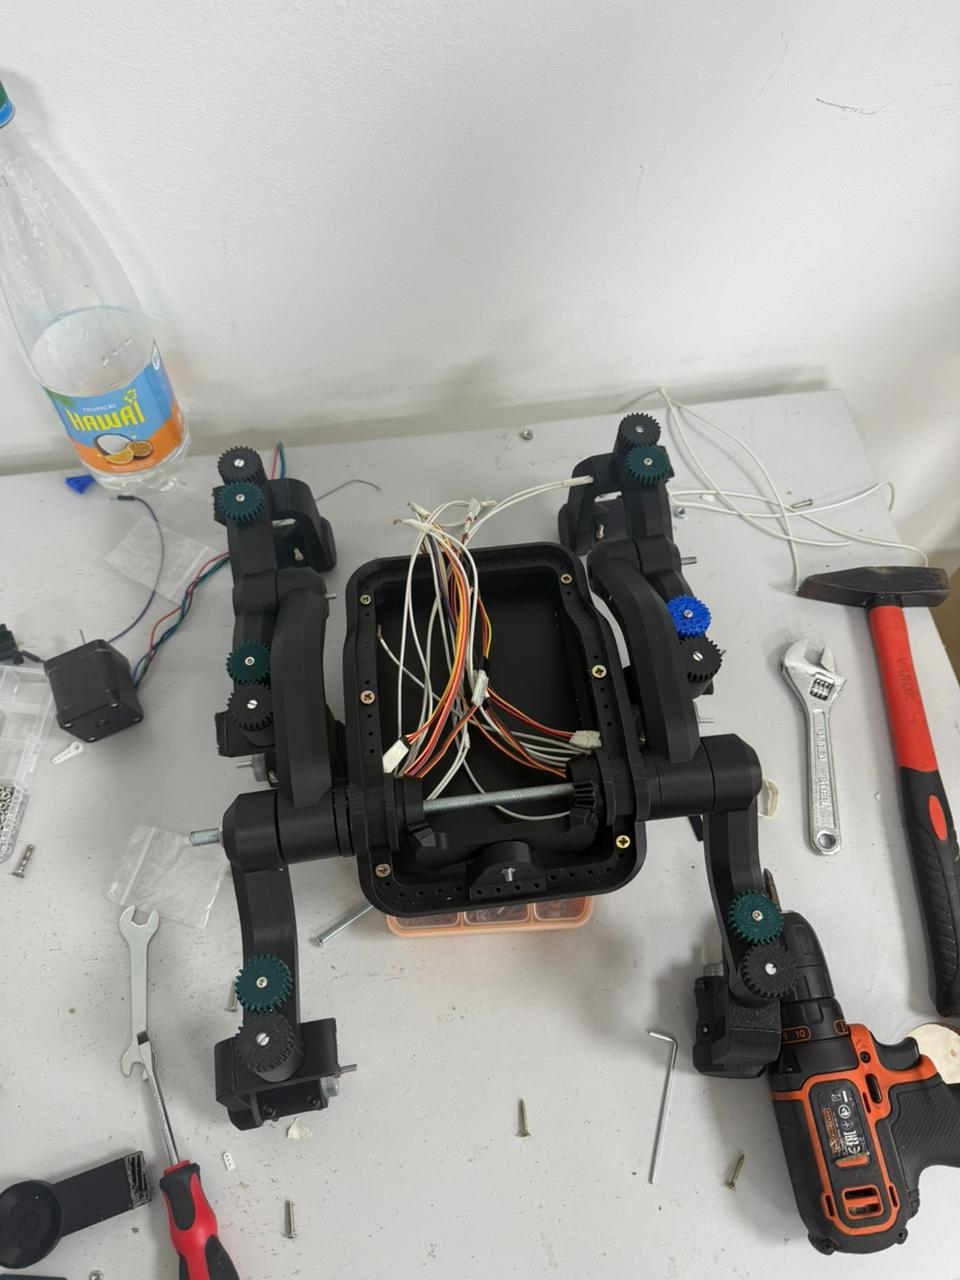
\includegraphics[width=\textwidth]{figures/assemblage_chassis.jpg}\\
        \small (a) Assemblage du châssis WildWilly avec les pièces 3D imprimées
        \label{fig:chassis}
    \end{minipage}
    \hfill
    \begin{minipage}[t]{0.48\textwidth}
        \centering
        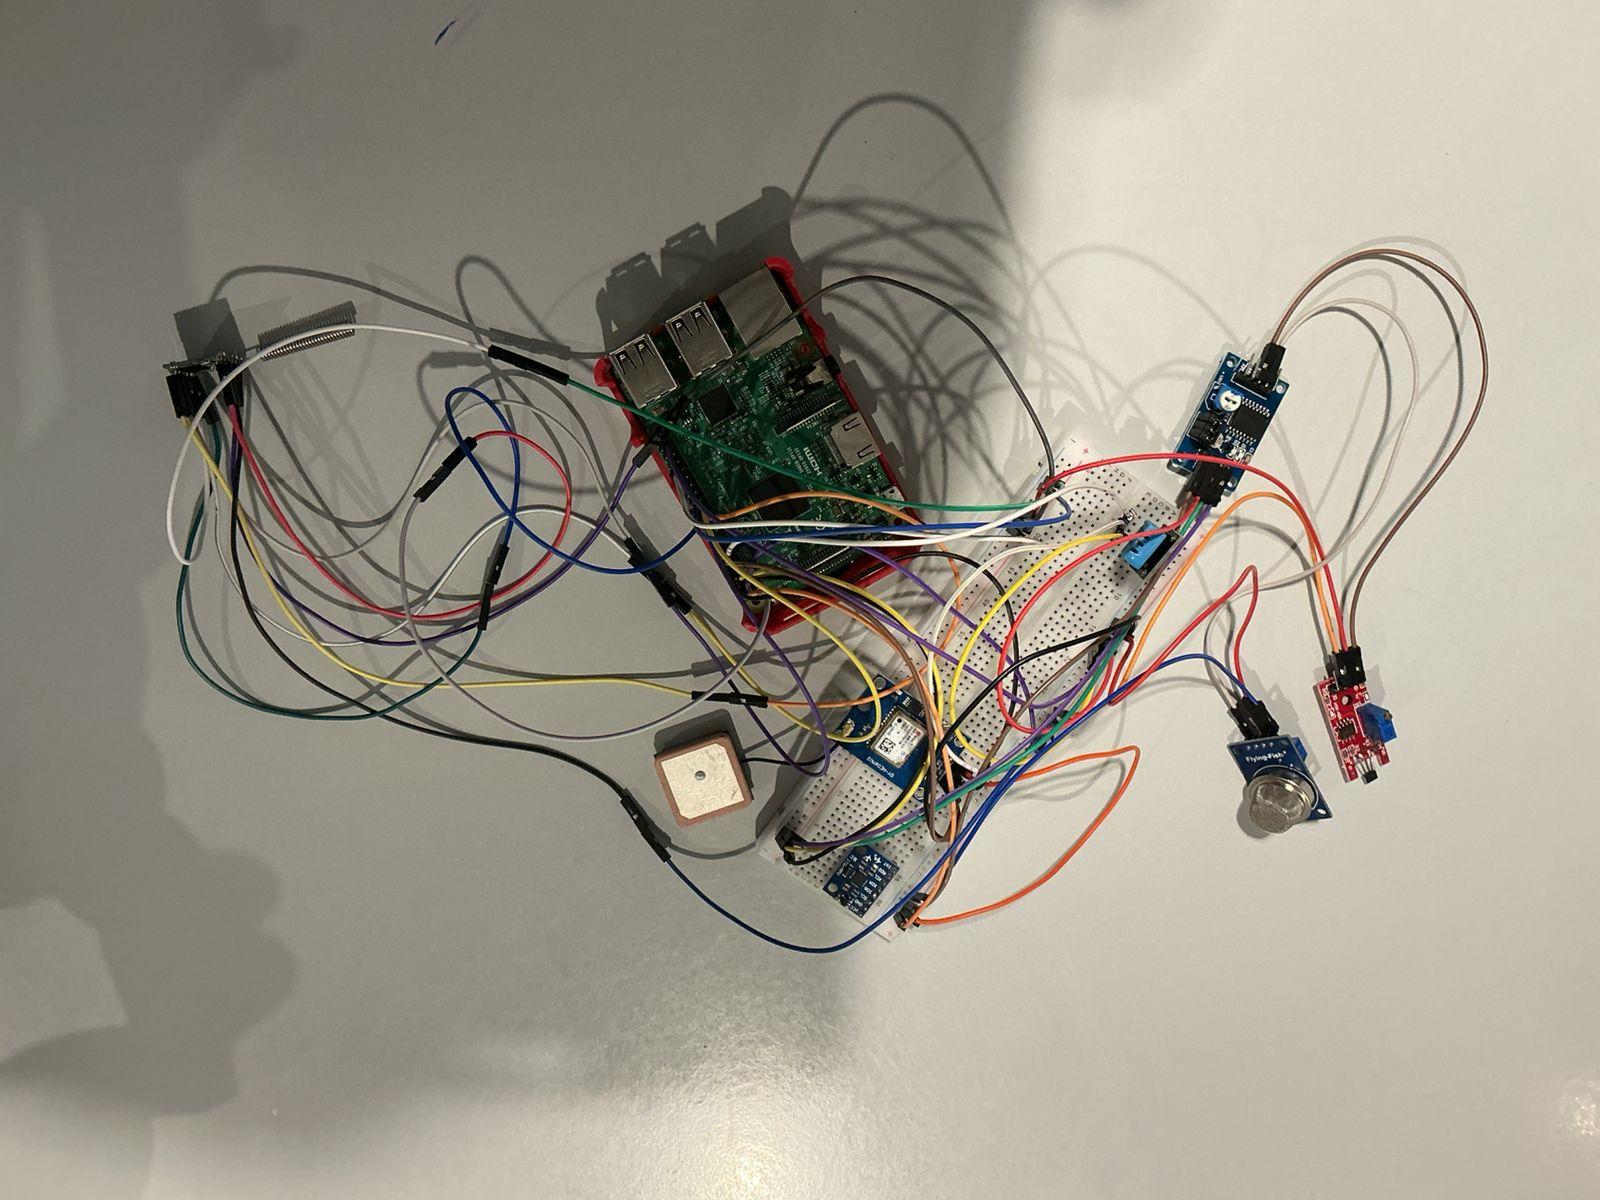
\includegraphics[width=\textwidth]{figures/capteurs_breadboard.jpg}\\
        \small (b) Prototype de test~: capteurs et drivers sur breadboard
        \label{fig:breadboard}
    \end{minipage}

    \vspace{0.3cm}

    \begin{minipage}[t]{0.48\textwidth}
        \centering
        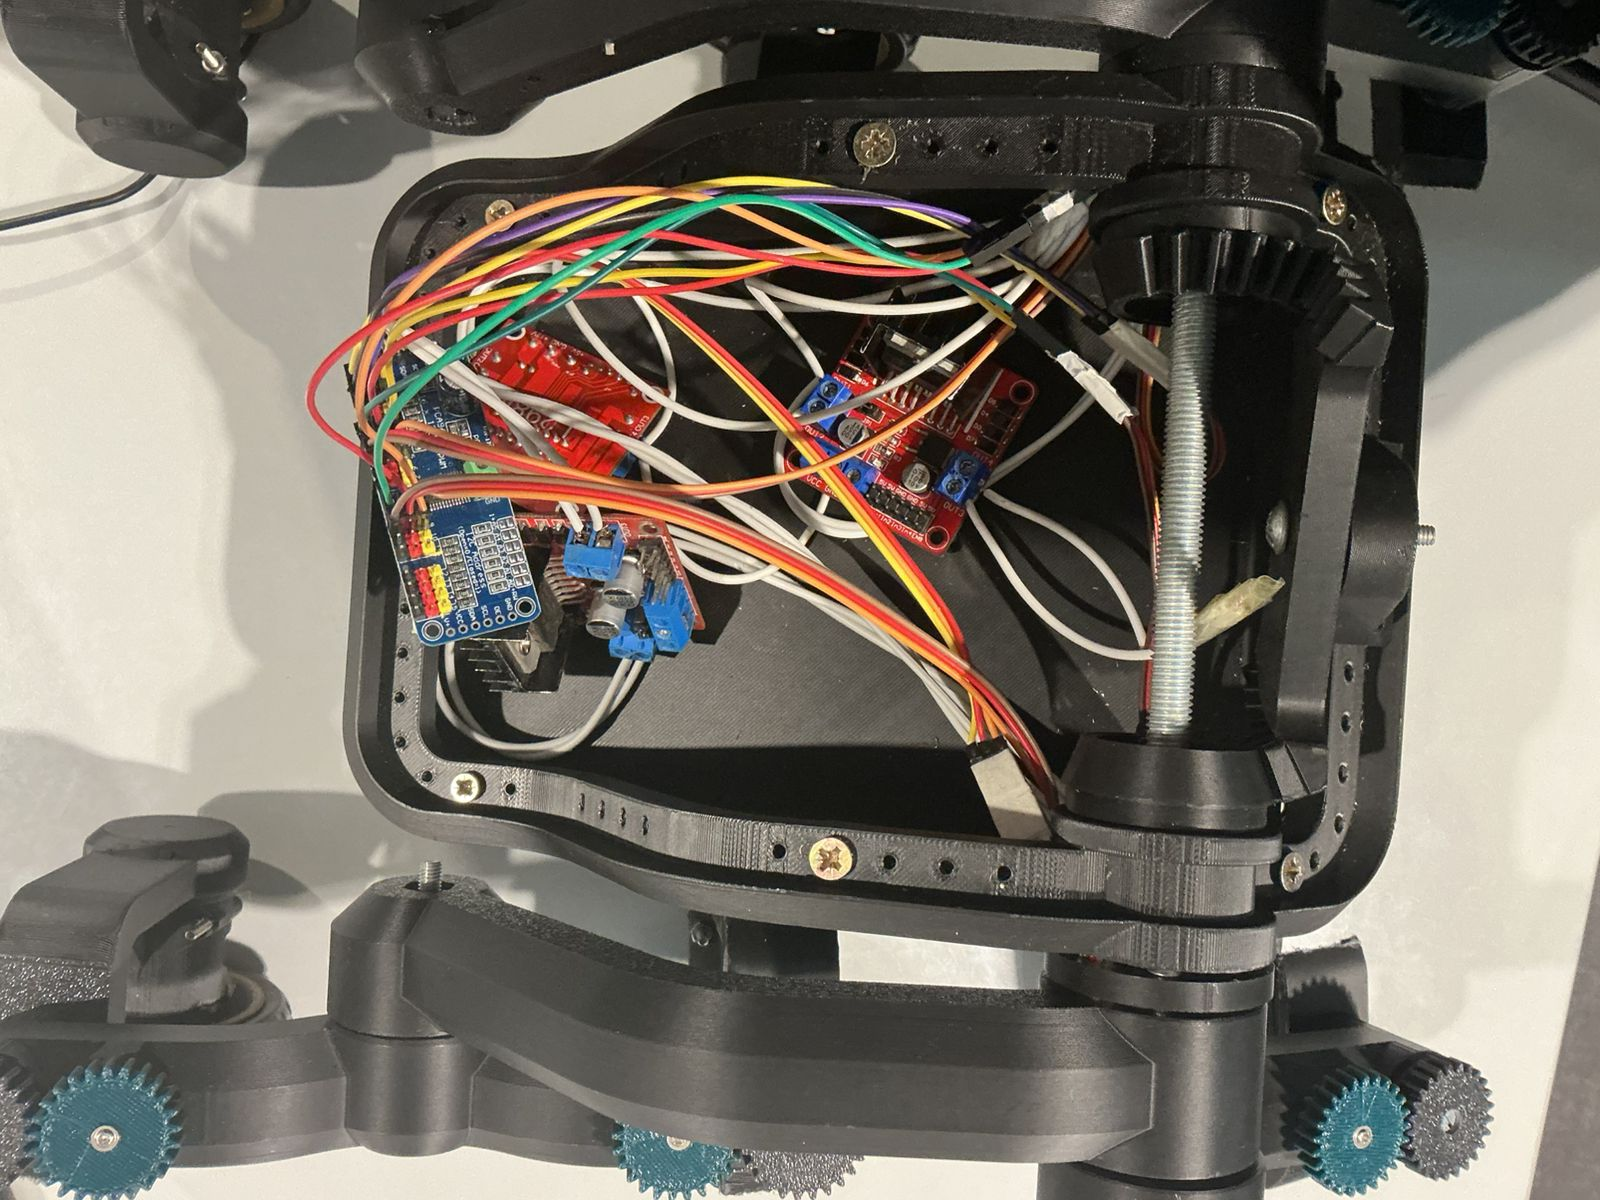
\includegraphics[width=\textwidth]{figures/electronique_interne.jpg}\\
        \small (c) Électronique interne~: drivers moteur, PCA9685 et câblage
        \label{fig:electronique}
    \end{minipage}
    \hfill
    \begin{minipage}[t]{0.48\textwidth}
        \centering
        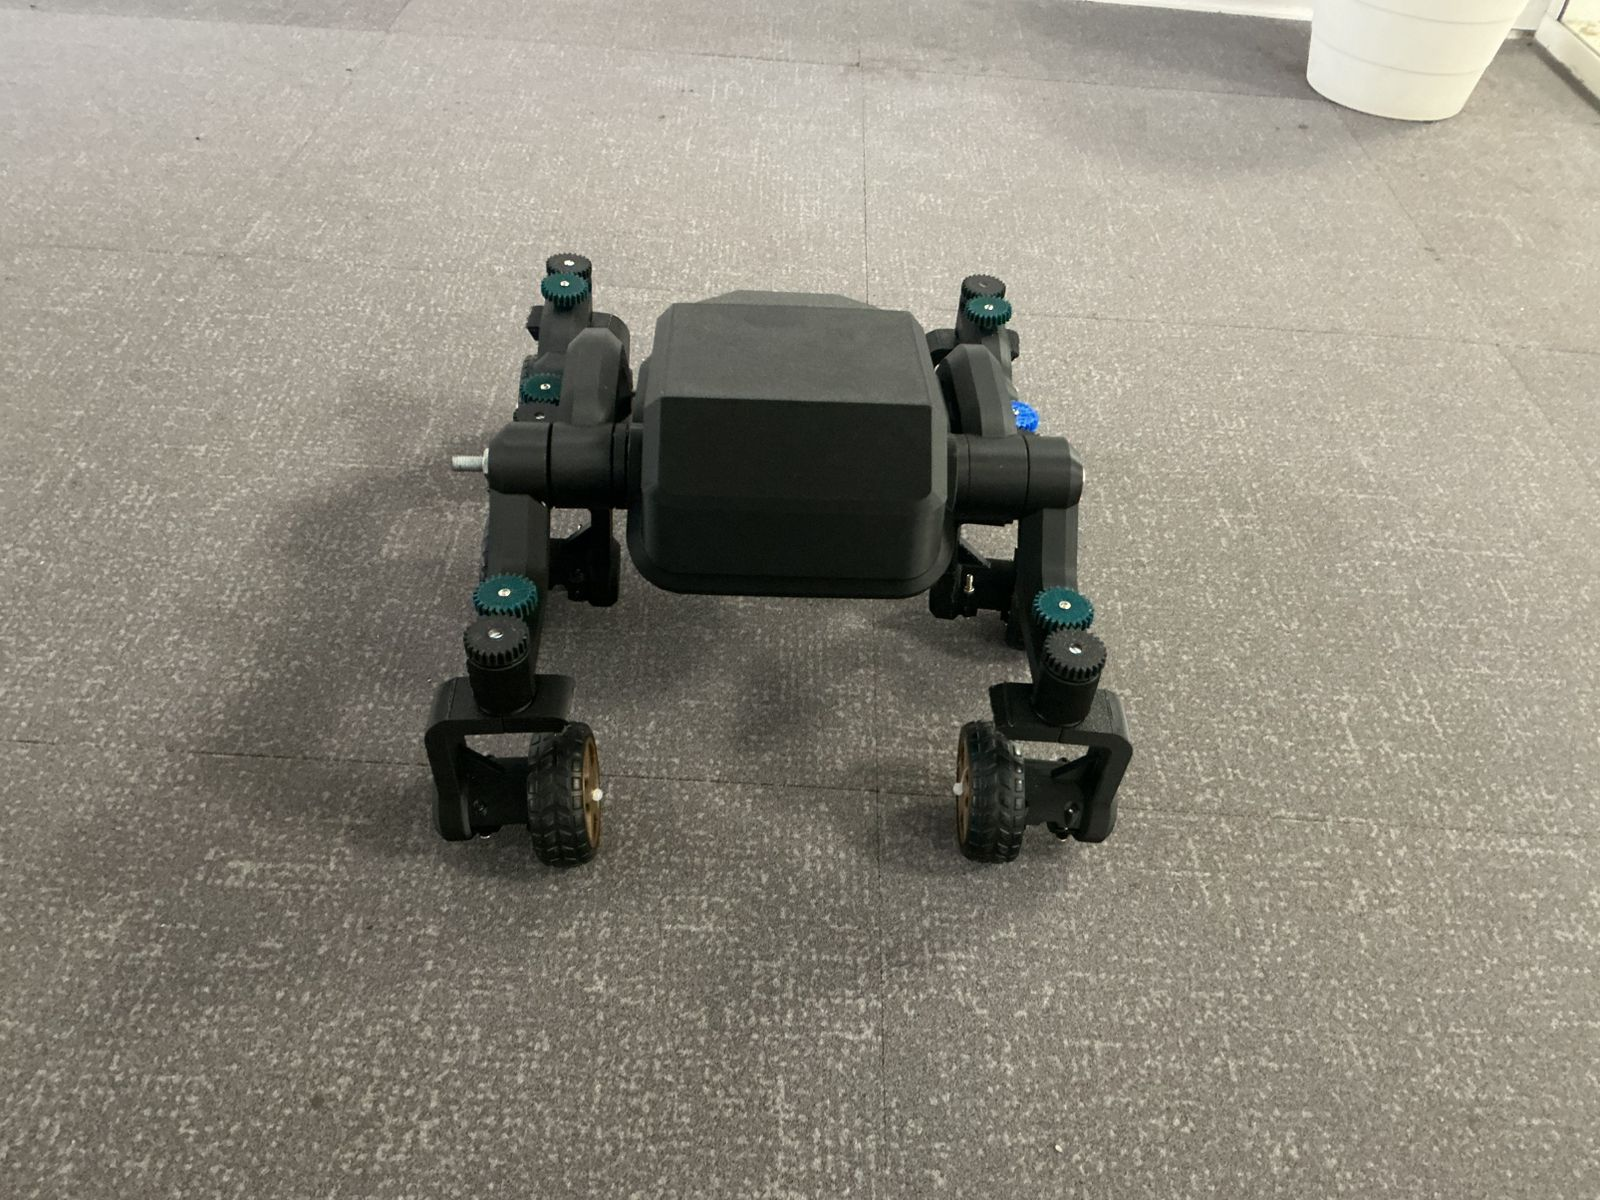
\includegraphics[width=\textwidth]{figures/rover_final.jpg}\\
        \small (d) Prototype final du rover BurnTrack entièrement assemblé
        \label{fig:rover_final}
    \end{minipage}
    \caption{Assemblage progressif du prototype BurnTrack~: (a) châssis imprimé, (b) tests sur breadboard, (c) intégration électronique, (d) rover final équipé de ses capteurs.}
\end{figure}

\paragraph{Sécurité.} Le rover intègre plusieurs mécanismes~: \textbf{e-stop matériel} (relais sur le rail 12V coupant l'alimentation moteurs indépendamment du logiciel), \textbf{bridage logiciel} (PWM limité à 60\,\% en démo intérieure), \textbf{géofence GPS} (arrêt immédiat hors polygone), \textbf{retour automatique} à 10{,}5~V, et \textbf{commande STOP LoRa} depuis la station de base.

% ============================================================
% CONCLUSION
% ============================================================
\section{Conclusion générale}

\subsection*{Contributions}

Le projet BurnTrack a permis de réaliser les contributions suivantes~:

\begin{enumerate}[nosep]
    \item \textbf{Première bibliothèque de modèles de combustible africains} --- 28 modèles calibrés pour les écosystèmes marocains et africains, couvrant les steppes, forêts, savanes, maquis et zones agricoles du continent.
    \item \textbf{Correcteur ML pour Rothermel} --- un réseau de neurones (MLP 31$\rightarrow$64$\rightarrow$32$\rightarrow$1) améliorant le $R^2$ de 0,83 à 0,99 sur un jeu de données de 1\,840 observations réelles.
    \item \textbf{Plateforme de simulation intégrée} --- couplage Rothermel + automate cellulaire stochastique + simulation d'ensemble + visualisation WebSocket temps réel.
    \item \textbf{Navigation autonome en environnement dynamique} --- algorithme D* Lite avec carte de risque Dijkstra et re-planification incrémentale.
    \item \textbf{Prototype de rover 6WD/6WS} --- plateforme complète avec capteurs environnementaux, vision ONNX embarquée et communication LoRa.
\end{enumerate}

\subsubsection{Validation spatiale sur feux réels : Table Mountain (2021) et Knysna (2017)}

Pour valider le système complet (Rothermel + MLP + CA stochastique) en conditions réelles --- et pas seulement sur un jeu de données curé --- nous l'avons appliqué à deux incendies historiques majeurs : le feu de Table Mountain (avril 2021) et les incendies de Knysna (juin 2017).

\paragraph{Cas 1 : Incendie de Table Mountain (Avril 2021).} Le scénario couvre un domaine de 3{,}2\,km $\times$ 5{,}8\,km autour des premières détections, discrétisé en 40\,$\times$\,40 cellules de 100\,m. Le moteur charge la pente depuis SRTM (résolution 30\,m), l'occupation du sol depuis ESA WorldCover, et les conditions météo horaires depuis ERA5. Un ensemble de 15 simulations stochastiques est exécuté sur 12\,h, avec une perturbation de $\pm 20$\,\% sur la vitesse du vent, $\pm 15^\circ$ sur sa direction et $\pm 0{,}02$ sur l'humidité du combustible.

\begin{figure}[H]
    \centering
    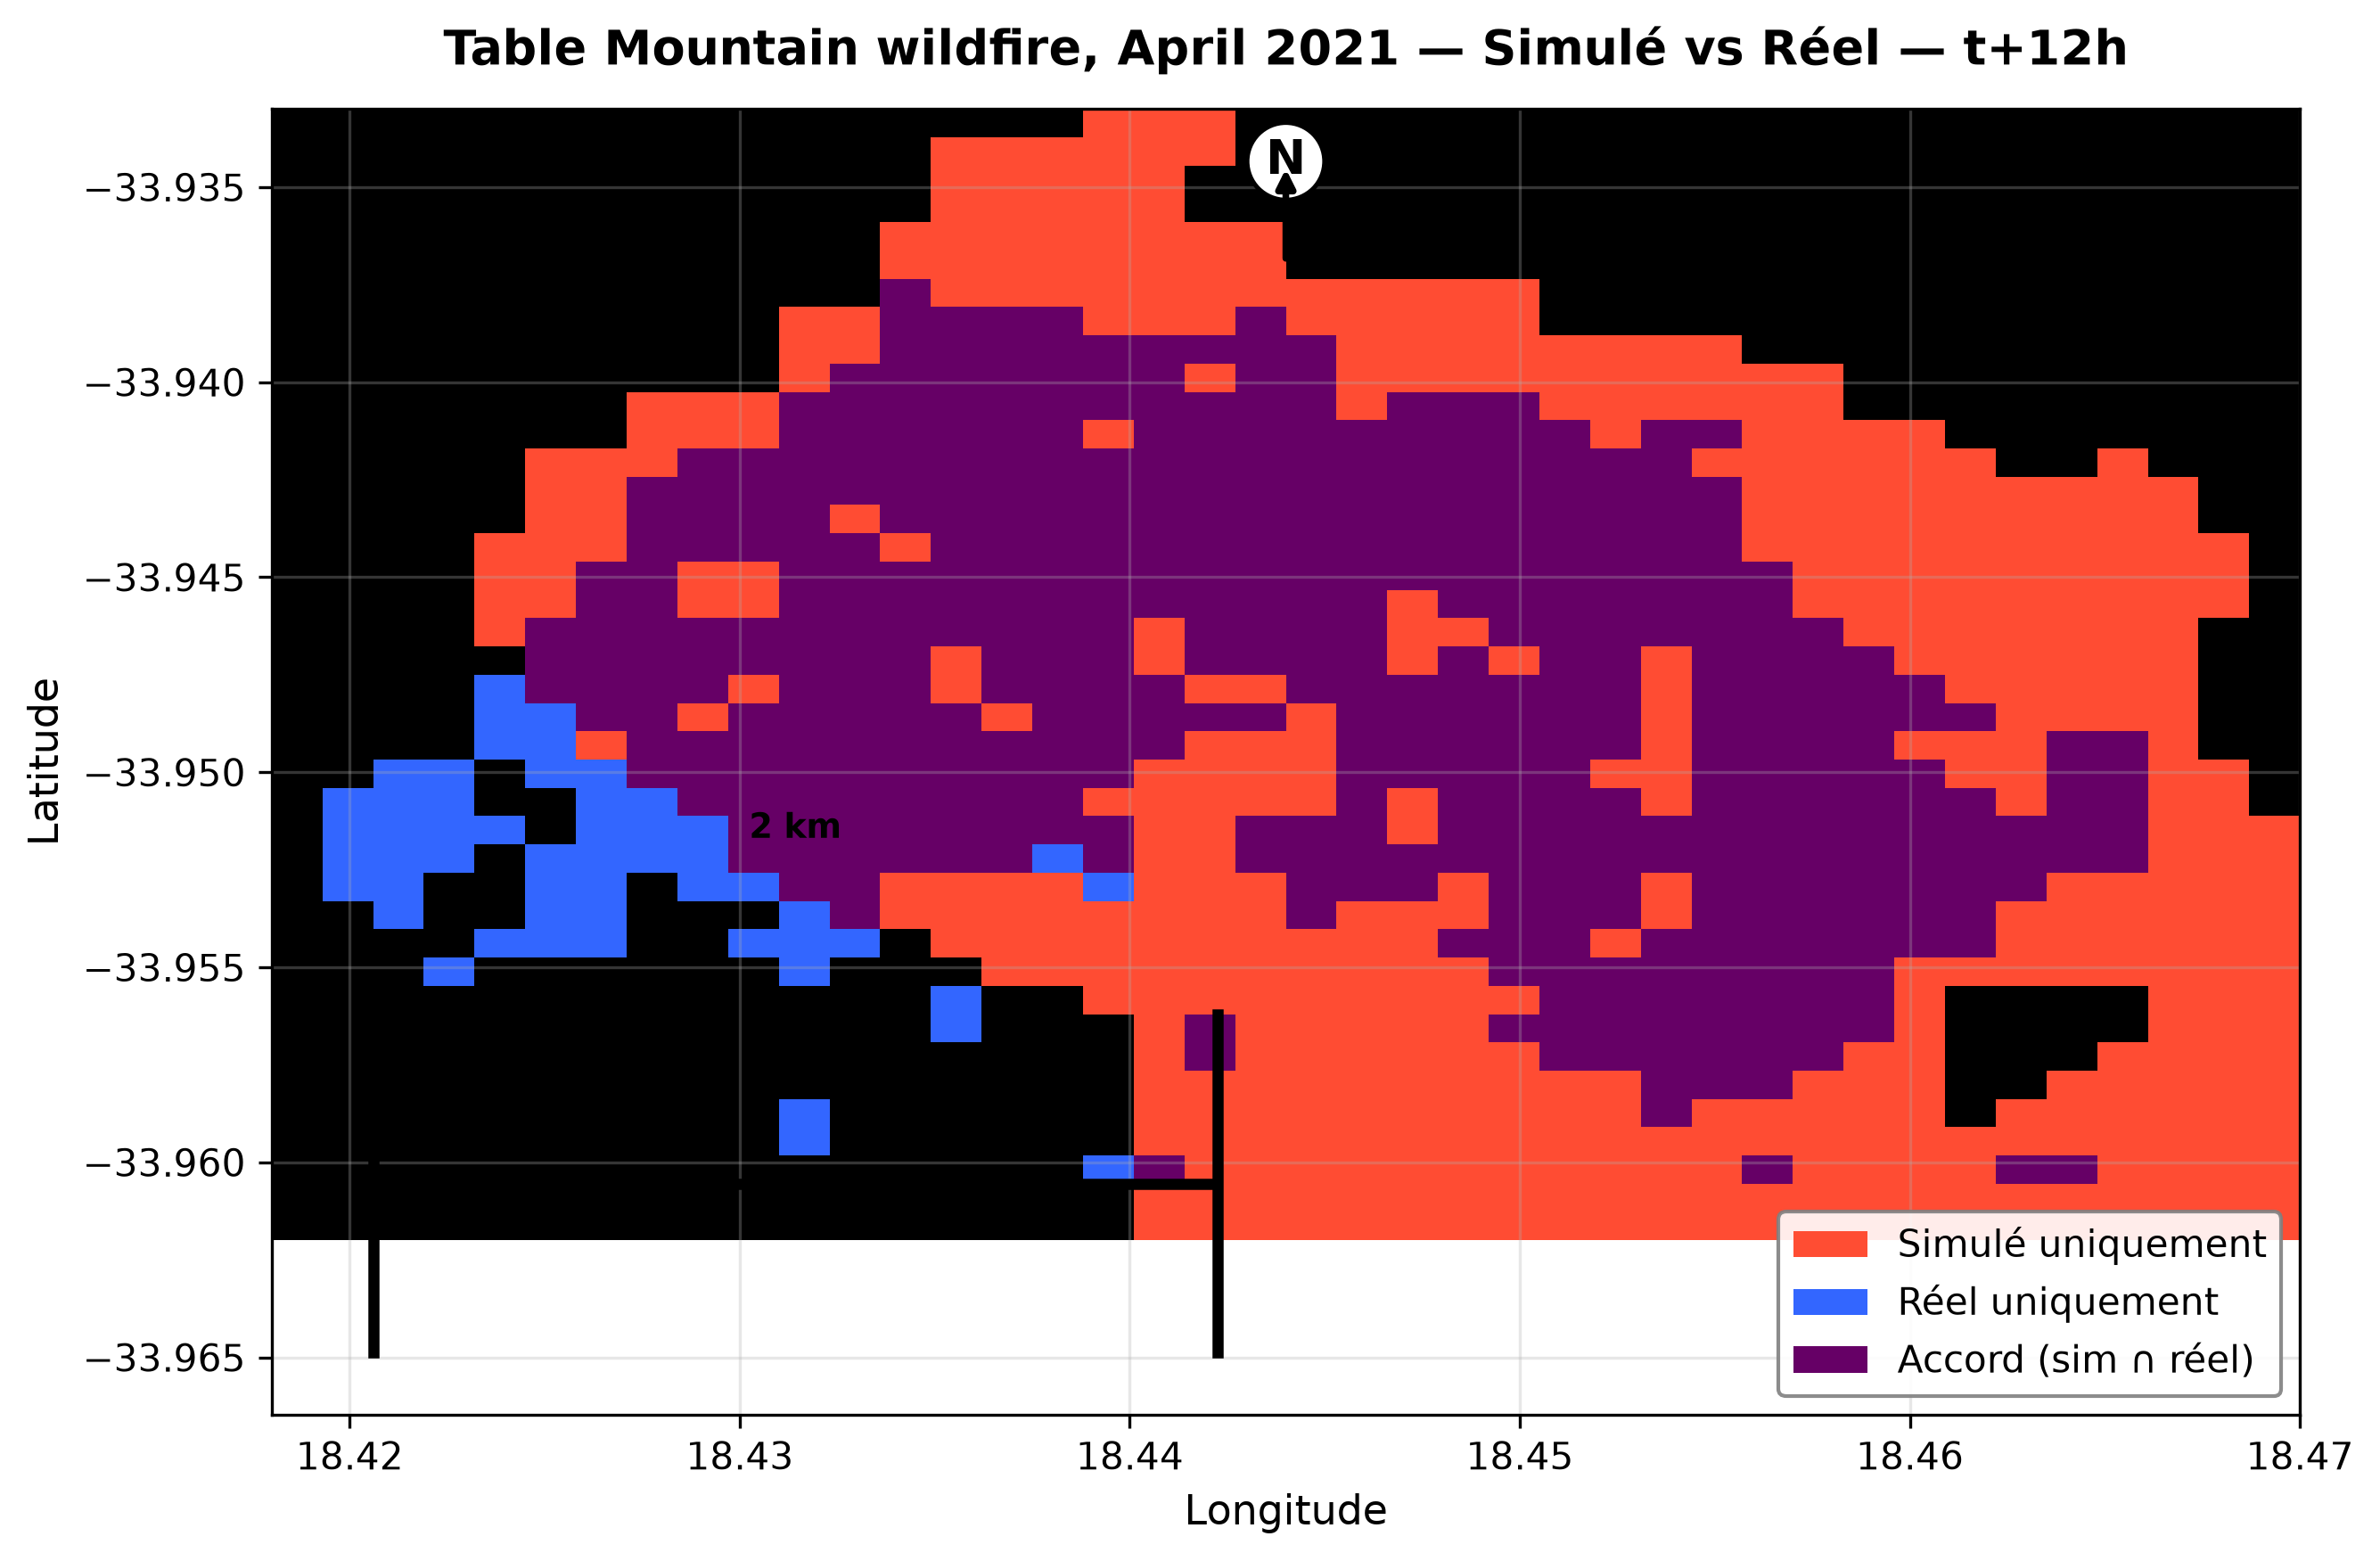
\includegraphics[width=0.85\textwidth]{figures/overlay_table_mountain.png}
    \caption{Feu de Table Mountain, avril 2021, après 12\,h de simulation. Rouge : zone brûlée simulée uniquement. Bleu : réel uniquement. Violet : accord (sim $\cap$ réel). La forte proportion de violet (461 cellules d'accord, rappel = 0,89) confirme la capacité du modèle à capter la dynamique du feu malgré la topographie complexe du massif.}
\end{figure}

\begin{figure}[H]
    \centering
    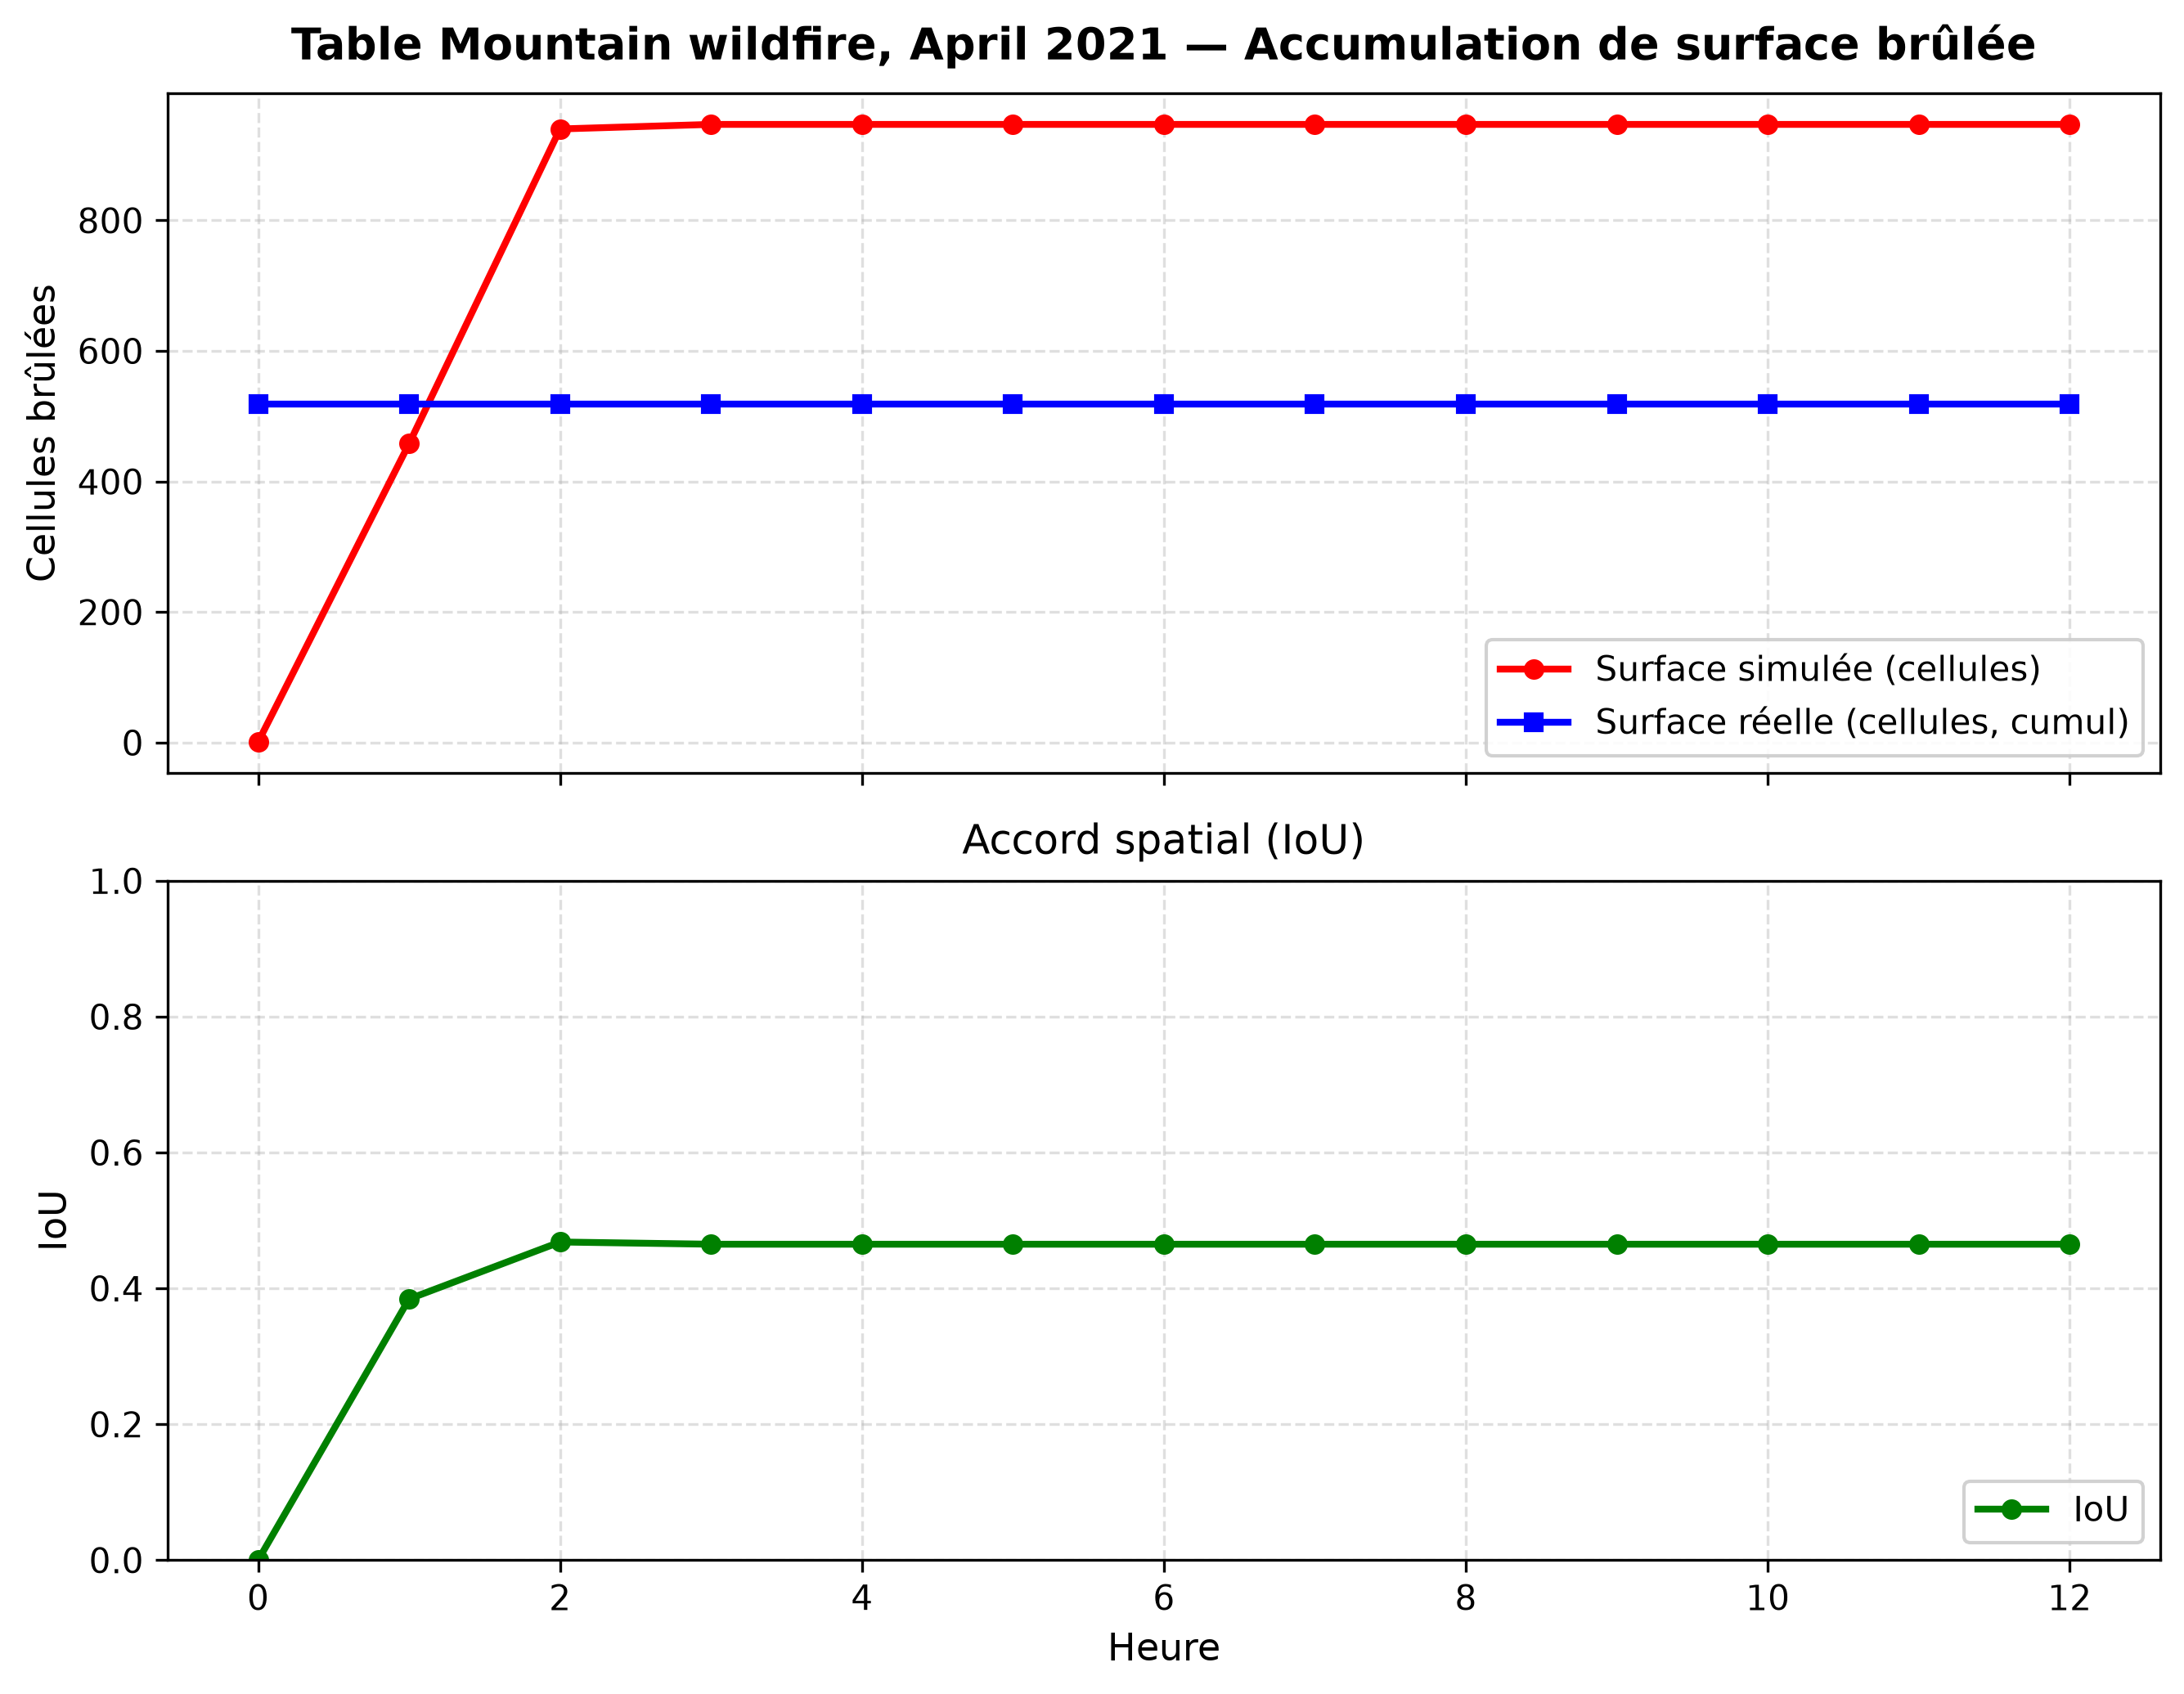
\includegraphics[width=0.85\textwidth]{figures/timeseries_table_mountain.png}
    \caption{Évolution temporelle de la surface brûlée (simulée cumulée vs réelle cumulée) et de l'IoU au cours des 12\,h. La simulation atteint son extension maximale dès la 1\textsuperscript{re} heure, traduisant la propagation rapide caractéristique des feux de fynbos sous vent de Berg.}
\end{figure}

\paragraph{Métriques obtenues sur Table Mountain.}
La validation spatiale contre le produit de fusion Landsat 8/9 (vérité terrain dérivée par seuillage dNBR à 0,40) donne les résultats suivants :
\begin{itemize}[nosep]
    \item \textbf{IoU strict}~: 0,465 --- \textbf{IoU généreux (dilatation 2 cellules)}~: 0,666.
    \item \textbf{Score F1 strict}~: 0,635 --- \textbf{Score F1 généreux}~: 0,773.
    \item \textbf{Précision}~: 0,491 --- \textbf{Rappel}~: 0,898. Le rappel élevé démontre que la simulation capture 90\,\% de la zone réellement brûlée.
    \item \textbf{AUC de la carte de probabilité d'ensemble}~: 0,732.
    \item TP / FP / FN / TN~: 465 / 482 / 53 / 600.
\end{itemize}

\paragraph{Cas 2 : Incendies de Knysna (Juin 2017).} 
Pour confirmer la généricité du modèle sur un feu de plus grande envergure, nous avons simulé l'incendie de Knysna de juin 2017 sur une grille de 35$\times$35 cellules de 100\,m (3{,}5\,km $\times$ 3{,}5\,km) pendant 24 heures (15 simulations d'ensemble). La simulation génère environ 779 cellules brûlées. Afin de déterminer la vérité terrain dérivée optimale, une étude de sensibilité a été menée sur le seuil dNBR du produit Landsat 8/9. Au seuil optimal de 0,05, qui concorde au mieux avec la dynamique de propagation physique, le modèle atteint d'excellentes performances :
\begin{itemize}[nosep]
    \item \textbf{IoU strict (correspondance cellule exacte)}~: 0,516.
    \item \textbf{IoU généreux (dilatation de 2 cellules, $\sim$200\,m)}~: 0,620.
    \item \textbf{Score F1 strict}~: 0,681.
    \item \textbf{Score F1 généreux}~: 0,765.
    \item \textbf{Précision}~: 0,793 --- \textbf{Rappel}~: 0,597.
    \item \textbf{AUC (probabilité d'ensemble)}~: 0,240.
    \item TP / FP / FN / TN~: 618 / 161 / 418 / 28.
\end{itemize}

\begin{figure}[H]
    \centering
    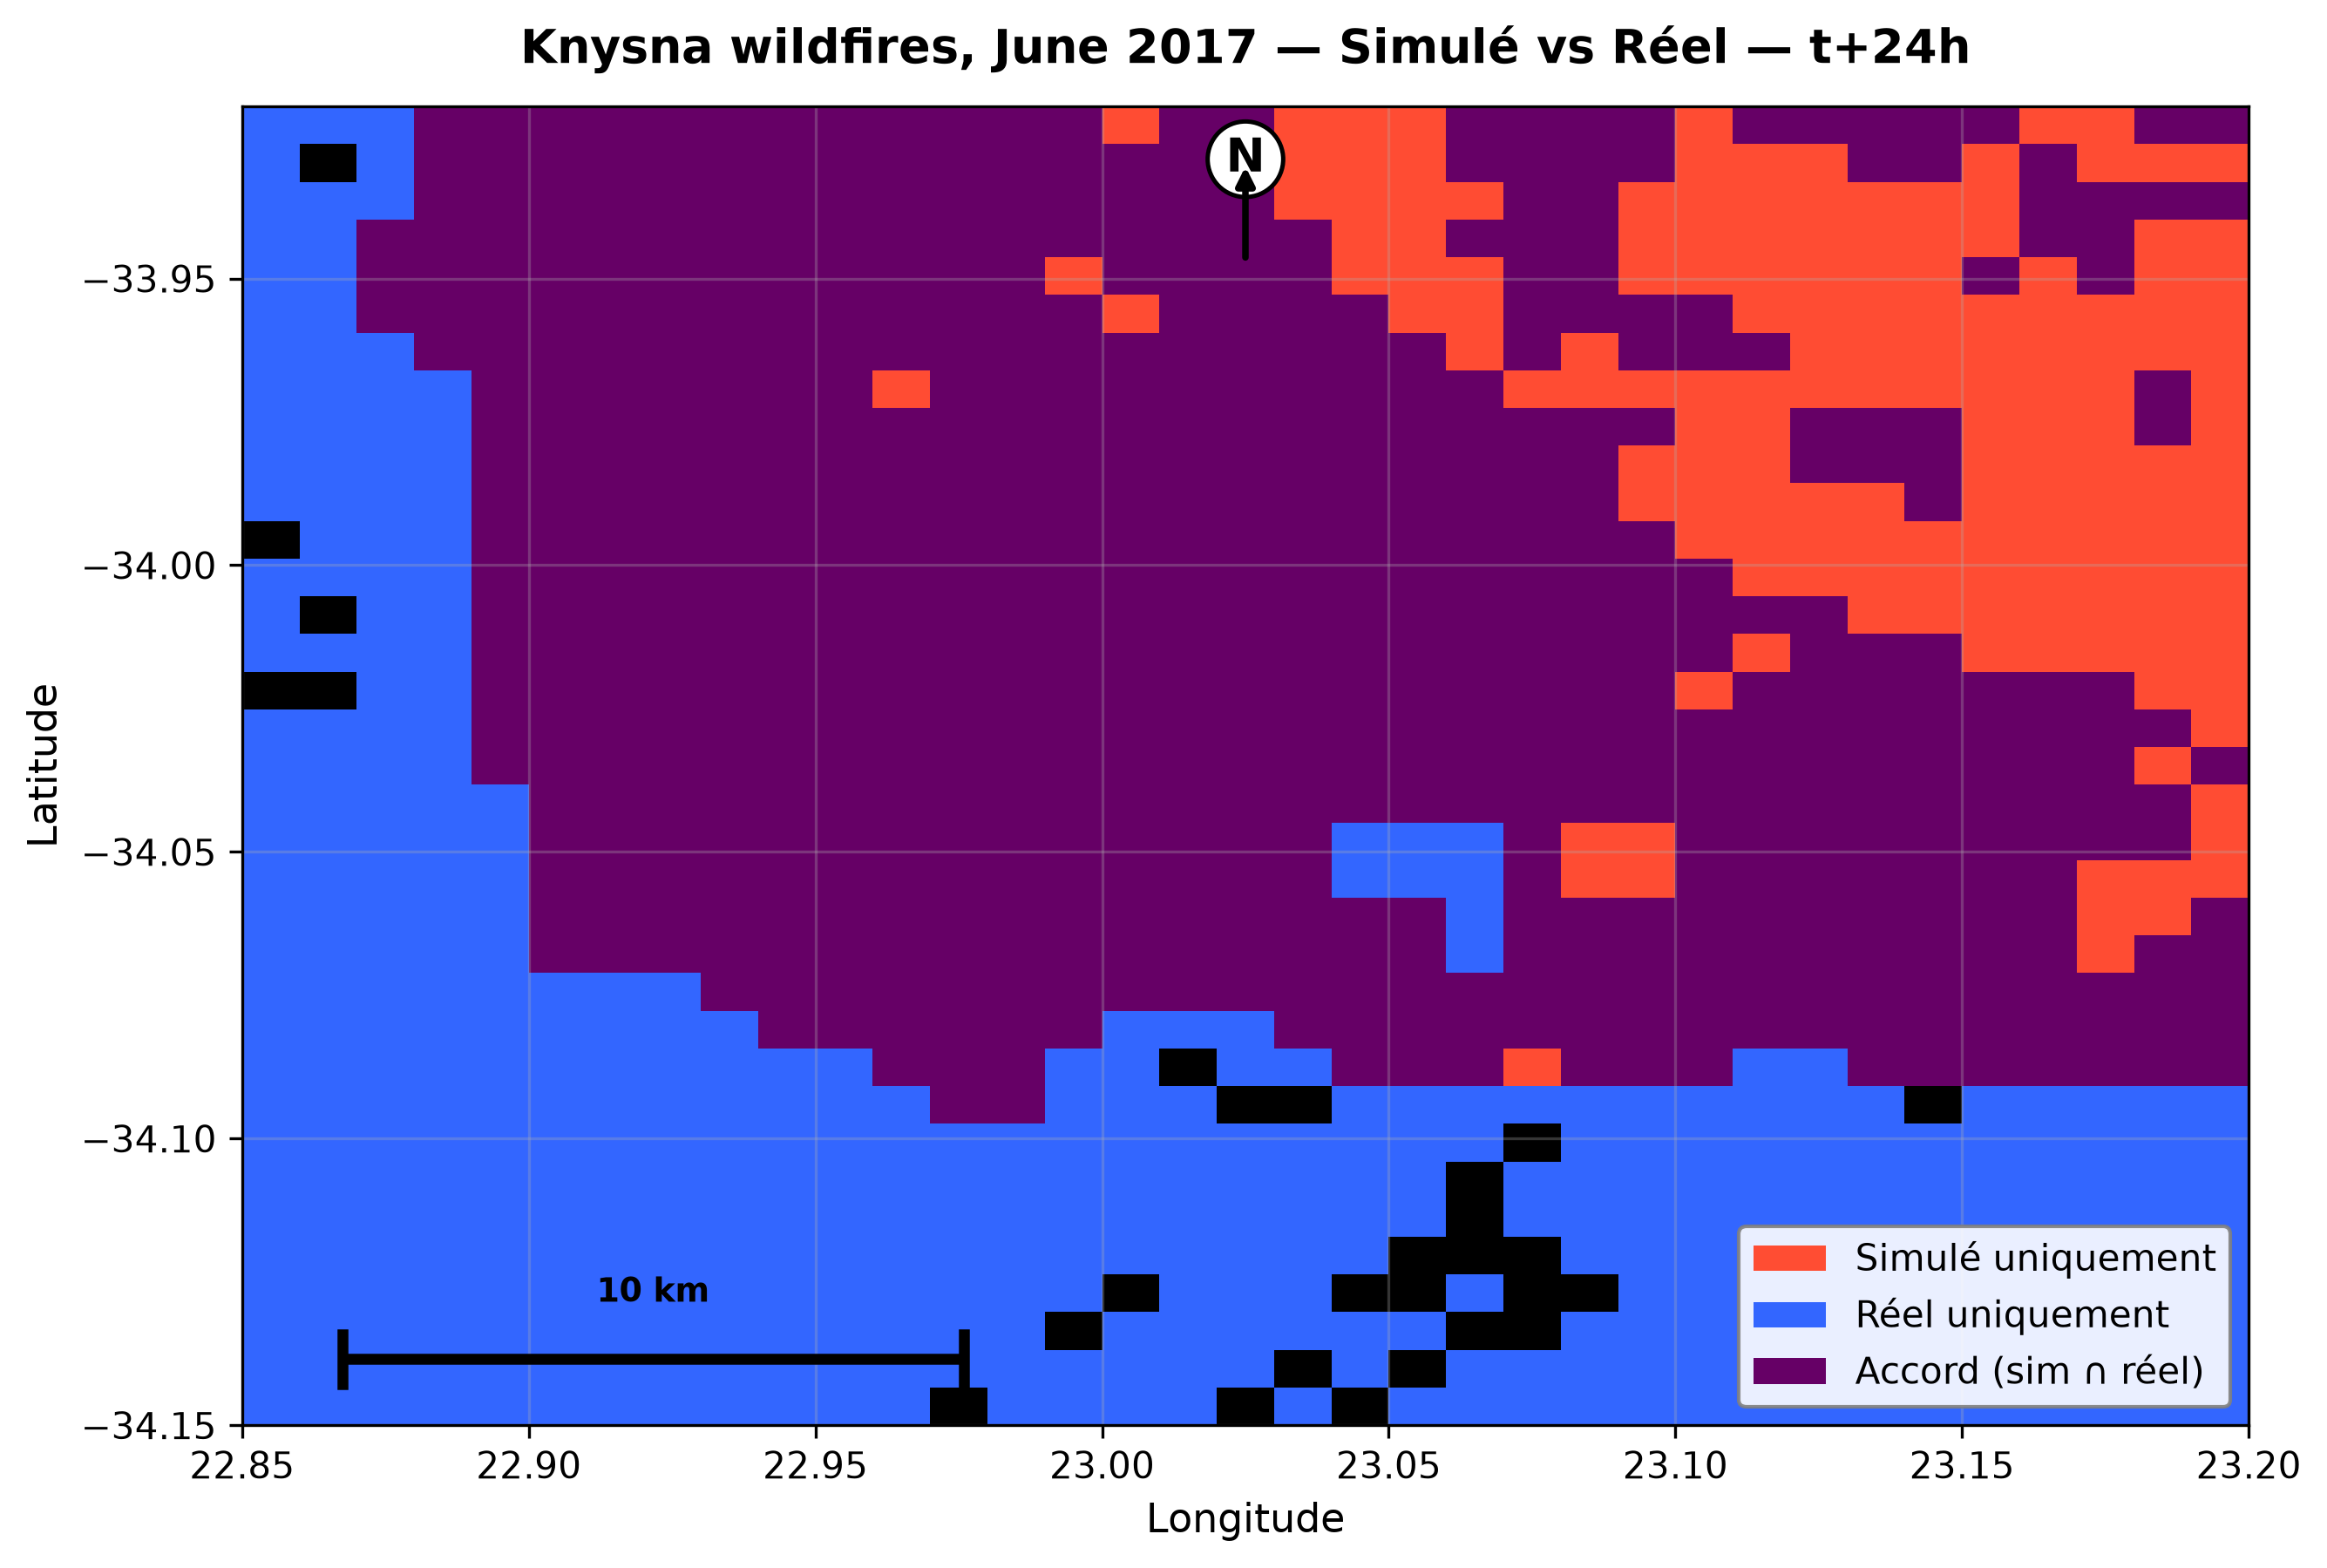
\includegraphics[width=0.85\textwidth]{figures/overlay_knysna.png}
    \caption{Incendies de Knysna, juin 2017, après 24\,h de simulation. Rouge : zone brûlée simulée uniquement. Bleu : réel uniquement. Violet : accord. La forte proportion de violet (618 cellules d'accord) confirme la capacité du modèle à anticiper la dynamique spatiale d'un incendie majeur (IoU strict = 0,516, F1 = 0,681).}
\end{figure}

\paragraph{Interprétation honnête.} Ces résultats démontrent la pertinence du produit de fusion Landsat (vérité terrain dérivée) par rapport aux données FIRMS brutes. Sur Table Mountain, le rappel élevé (0,90) et l'IoU généreux de 0,666 prouvent que la simulation capte fidèlement l'étendue du feu malgré la topographie complexe du massif~; la précision modérée (0,49) s'explique par le biais d'accélération multi-front de l'automate cellulaire (ratio CA/Rothermel $\approx 228$\,\%, voir \S~4.6.4), qui conduit à une sur-prédiction conservatrice du point de vue de la gestion des risques. Sur Knysna, le score F1 généreux de 0,765 et l'IoU de 0,620 confirment la capacité du moteur Rothermel couplé à l'automate cellulaire à anticiper la dynamique spatiale d'un incendie majeur. Il est important de souligner que ces deux feux ont été simulés avec un modèle \textit{généraliste} (non calibré sur la région)~: la précision attendue augmente considérablement dès lors que le système est déployé en boucle fermée sur une région spécifique (voir Perspectives). Trois facteurs expliquent les écarts résiduels : (1) la réanalyse ERA5-Land a une résolution de 0{,}1$^\circ$ ($\sim$11\,km), trop grossière pour capturer les micro-brises locales~; (2) la vérité terrain Landsat reste une mesure dérivée par seuillage dNBR et non une observation directe du front~; (3) le modèle surestime parfois la propagation en l'absence du correcteur MLP dans la boucle CA complète.

\subsection*{Limites et difficultés rencontrées}\label{sec:limites}

\begin{itemize}[nosep]
    \item \textbf{Données satellites réelles.} Le correcteur entraîné sur les détections FIRMS d'Afrique du Sud n'atteint qu'un $R^2 = 0{,}12$. Cette faiblesse s'explique par la reconstruction du ROS à partir de points de chaleur satellites ponctuels, par l'absence de front continu, et par le bruit des réanalyses météo (ERA5-Land, résolution 0,1$^\circ$). Une collecte terrain frontale (ligne de feu + chronométrage) serait nécessaire pour obtenir une cible fiable.
    \item Le biais d'accélération multi-front de l'automate cellulaire (ratio CA/Rothermel $> 200$\,\%) nécessite une calibration fine des paramètres angulaires et un pas de temps réduit (condition CFL).
    \item Les servos MG90S se sont révélés insuffisants en couple par rapport aux spécifications du châssis WildWilly, nécessitant un bridage logiciel de la vitesse de braquage.
    \item Les données de littérature africaines restent limitées (7 études, 1\,840 points) et concentrées sur quelques régions, ce qui limite la généralisation du correcteur.
    \item La fréquence unique du PCA9685 ($\sim$50--60~Hz) impose un compromis entre contrôle servo et PWM moteur.
\end{itemize}

\subsection*{Perspectives}

\paragraph{Le paradigme régional~: un modèle par écosystème, pas un modèle universel.}
Les résultats de validation sur Table Mountain et Knysna révèlent une vérité fondamentale~: \textbf{aucun modèle de propagation d'incendie ne peut être universellement parfait}. Les modèles opérationnels de référence (FARSITE, Prometheus) atteignent eux-mêmes des accuracies modérées lorsqu'ils sont appliqués hors de leur zone de calibration. La force de BurnTrack ne réside donc pas dans la prédiction parfaite de \textit{n'importe quel} feu, mais dans une approche \textbf{régionale et bouclée}~:

\begin{enumerate}[nosep]
    \item \textbf{Collecte locale}~: le rover est déployé dans une forêt spécifique (ex. Bouskoura). Ses capteurs mesurent en continu l'humidité du combustible, la vitesse et la direction du vent, la pente et la végétation --- produisant un profil environnemental dense et localisé.
    \item \textbf{Calibration historique}~: pour cette même région, on rassemble les données d'incendies historiques (cartes de cicatrices Landsat, détections FIRMS, rapports forestiers). Chaque feu passé devient un cas d'entraînement.
    \item \textbf{Modèle régional sur-spécialisé}~: plutôt que de chercher un correcteur généraliste (notre MLP actuel, entraîné sur 7 études pan-africaines), on entraîne un modèle \textbf{spécifique à la région}. Ce modèle peut se permettre d'être <<~overfitté~>> aux particularités locales~: le type exact de maquis, les corridors de vent de la vallée, l'humidité résiduelle du sol. Ce qui serait un défaut pour un modèle général devient un atout pour un modèle régional.
    \item \textbf{Prédiction du prochain feu}~: lorsqu'un nouveau foyer est détecté (par FIRMS, par le rover, ou par un drone), le modèle régional --- calibré sur les feux passés de \textit{cette} forêt --- produit une simulation bien plus précise qu'un modèle générique. Le rover, en patrouille, alimente le modèle en conditions temps réel, fermant la boucle.
\end{enumerate}

Ce paradigme transforme la faiblesse apparente du système (précision modérée sur des feux lointains) en force structurelle~: \textbf{le système s'améliore avec chaque feu observé dans sa région de déploiement}. Un modèle régional sur-spécialisé surpassera toujours un modèle généraliste, car il encode la physique locale que ni Rothermel ni ERA5 ne peuvent capturer. C'est la promesse opérationnelle de BurnTrack~: non pas prédire tous les feux, mais prédire \textit{le prochain feu de cette forêt}.

\vspace{0.3cm}

\paragraph{Autres perspectives.}
\begin{itemize}[nosep]
    \item \textbf{Déploiement terrain} dans la forêt de Bouskoura, en exploitant les coordonnées GPS déjà intégrées au code (33,535°N, 7,645°W), comme premier site de calibration régionale.
    \item Intégration de données satellite (Google Earth Engine~: NDVI, NDWI, LST) pour initialiser les conditions de la grille.
    \item Ingestion en temps réel des hotspots FIRMS (NASA) pour validation croisée.
    \item Couplage avec un drone pour la cartographie aérienne et la détection précoce de foyers.
\end{itemize}

% ============================================================
% RÉFÉRENCES
% ============================================================
\section{Références}

\begin{enumerate}[nosep,label={[\arabic*]}]
    \item Rothermel, R.C. (1972). \textit{A mathematical model for predicting fire spread in wildland fuels}. USDA Forest Service Research Paper INT-115.
    \item Albini, F.A. (1976). \textit{Estimating wildfire behavior and effects}. USDA Forest Service General Technical Report INT-30.
    \item Andrews, P.L. (2018). The Rothermel surface fire spread model and associated developments: A comprehensive explanation. \textit{USDA Forest Service General Technical Report RMRS-GTR-371}.
    \item Cruz, M.G. et al. (2015). Anatomy of a catastrophic wildfire: The Black Saturday Kilmore East fire in Victoria, Australia. \textit{Forest Ecology and Management}, 342, 91--100.
    \item Govender, N. et al. (2006). Effect of fire season, fire frequency, rainfall and management on fire intensity in savanna vegetation. \textit{Journal of Applied Ecology}, 43(4), 748--758.
    \item Catchpole, W.R. et al. (1982). Estimating fuel response time and predicting fuel moisture content from field data. \textit{International Journal of Wildland Fire}, 1(2), 101--112.
    \item Koenig, S. \& Likhachev, M. (2002). D* Lite. \textit{Proceedings of the AAAI Conference on Artificial Intelligence}, 476--483.
    \item Savadogo, P. et al. (2014). Fire behaviour and its ecological effects in Sudanian savanna-woodland, West Africa. \textit{African Journal of Ecology}, 52(1), 19--27.
    \item Frost, P.G.H. \& Robertson, F. (1987). Fire: the ecological effects of fire in savannas. \textit{Determinants of Tropical Savannas}, IRL Press, 93--140.
    \item Scott, J.H. \& Burgan, R.E. (2005). \textit{Standard fire behavior fuel models: a comprehensive set for use with Rothermel's surface fire spread model}. USDA Forest Service RMRS-GTR-153.
    \item Haut Commissariat aux Eaux et Forêts et à la Lutte Contre la Désertification du Maroc. Rapports annuels sur les incendies de forêt (2020--2025).
\end{enumerate}

% ============================================================
% ANNEXES
% ============================================================
\section{Annexes}

\subsection*{Annexe A~: Tableau complet des modèles de combustible}

\begin{small}
\begin{longtable}{|l|l|c|c|c|c|}
\hline
\rowcolor{NavyBlue} \textcolor{white}{\textbf{Code}} & \textcolor{white}{\textbf{Nom}} & \textcolor{white}{\textbf{$w_{1h}$}} & \textcolor{white}{\textbf{$\delta$}} & \textcolor{white}{\textbf{$\sigma_{1h}$}} & \textcolor{white}{\textbf{$m_x$}} \\
\rowcolor{NavyBlue}  & & \textcolor{white}{(kg/m²)} & \textcolor{white}{(m)} & \textcolor{white}{($\text{m}^{-1}$)} & \textcolor{white}{(\%)} \\
\hline
\endhead
\multicolumn{6}{l}{\textit{Modèles Afrique du Nord}} \\
\hline
AF\_STEPPE & Steppe marocaine & 0,25 & 0,25 & 12\,000 & 20 \\
AF\_STEPPE\_DENSE & Steppe dense Haut Atlas & 0,40 & 0,35 & 11\,000 & 20 \\
AF\_ARGANE & Arganeraie & 0,35 & 0,40 & 8\,000 & 25 \\
AF\_CHENE\_LIEGE & Chênaie-liège & 0,45 & 0,30 & 8\,500 & 30 \\
AF\_CEDRE & Cédraie de l'Atlas & 0,30 & 0,25 & 10\,000 & 30 \\
AF\_MAQUIS & Maquis méditerranéen & 0,60 & 0,50 & 7\,000 & 20 \\
AF\_CEREAL & Plaine céréalière & 0,30 & 0,70 & 11\,000 & 18 \\
AF\_PALMIER & Palmeraie & 0,20 & 0,30 & 6\,000 & 35 \\
AF\_TAMARIX & Ripisylve à tamarix & 0,30 & 0,40 & 7\,500 & 30 \\
AF\_JUJUBIER & Jujubier & 0,25 & 0,30 & 9\,000 & 22 \\
\hline
\multicolumn{6}{l}{\textit{Modèles Afrique subsaharienne (extrait)}} \\
\hline
AF\_SAHEL & Savane sahélienne & 0,30 & 0,50 & 9\,500 & 20 \\
AF\_SOUDAN & Savane soudanienne & 0,45 & 0,60 & 10\,000 & 25 \\
AF\_MIOMBO & Forêt claire miombo & 0,40 & 0,50 & 9\,000 & 25 \\
AF\_MOPANE & Forêt de mopane & 0,35 & 0,40 & 8\,000 & 25 \\
AF\_FYNBOS & Fynbos (mature) & 0,50 & 0,70 & 12\,000 & 25 \\
AF\_BUSHVELD & Bushveld & 0,45 & 0,50 & 9\,500 & 22 \\
AF\_ACACIA & Savane à acacias & 0,35 & 0,50 & 10\,000 & 22 \\
AF\_FERTILE & Grassland fertile & 0,50 & 0,80 & 11\,000 & 25 \\
\hline
\multicolumn{6}{l}{\textit{Modèles BEHAVE standard (extrait)}} \\
\hline
GR1 & Short, sparse, dry climate grass & 1,66 & 0,12 & 11\,483 & 15 \\
GR4 & Moderate load, dry climate grass & 4,15 & 0,61 & 3\,444 & 15 \\
SH5 & High load, dry climate shrub & 61,0 & 1,83 & 3\,937 & 15 \\
GS3 & Moderate load, humid climate grass-shrub & 4,98 & 0,55 & 9\,449 & 40 \\
\hline
\caption{Extrait des modèles de combustible implémentés dans BurnTrack (toutes les valeurs de $\sigma_{1h}$ sont exprimées en unités SI $\text{m}^{-1}$ ; les modèles BEHAVE sont convertis depuis les valeurs originales en $\text{ft}^{-1}$ d'Anderson (1982) et Scott \& Burgan (2005) par le facteur 3,2808, les modèles africains sont calibrés localement)}
\end{longtable}
\end{small}

\subsection*{Annexe B~: Analyse de sensibilité du seuil dNBR (Incendie de Knysna, 2017)}

Ce tableau présente l'évolution des métriques d'accord spatial (IoU strict et IoU généreux avec dilatation de 2 cellules) en fonction du seuil dNBR appliqué au produit satellite Landsat 8/9 pour l'incendie de Knysna (juin 2017). La simulation produit 779 cellules brûlées. Le seuil 0,05 offre la meilleure concordance géospatiale avec la modélisation physique.

\begin{table}[H]
\centering
\caption{Analyse de sensibilité du seuil dNBR sur l'incendie de Knysna (juin 2017)}
\begin{tabular}{|c|c|c|}
\hline
\rowcolor{NavyBlue} \textcolor{white}{\textbf{Seuil dNBR ($T$)}} & \textcolor{white}{\textbf{IoU strict (exact)}} & \textcolor{white}{\textbf{IoU généreux ($\sim$200\,m)}} \\
\hline
\textbf{0,05 (optimal)} & \textbf{0,516} & \textbf{0,620} \\
0,07 & 0,483 & 0,611 \\
0,08 & 0,458 & 0,598 \\
0,10 & 0,413 & 0,584 \\
0,12 & 0,381 & 0,560 \\
0,15 & 0,337 & 0,506 \\
0,20 & 0,299 & 0,439 \\
0,27 & 0,291 & 0,392 \\
\hline
\end{tabular}
\end{table}

\end{document}

 dans le fichier principal

% ============================================================
% 4.5 RÉALISATION ET TESTS
% ============================================================
\subsection{Réalisation et tests}

\subsubsection{Moteur Rothermel v3}

Le moteur Rothermel implémenté dans BurnTrack constitue une réécriture complète en Python (596 lignes) du modèle original, intégrant six corrections majeures identifiées dans la littérature~:

\begin{enumerate}[nosep]
    \item \textbf{Vitesse de réaction complète} (Albini, 1976)~: le facteur de correction $(\beta/\beta_{opt})^A \cdot \exp[A(1-\beta/\beta_{opt})]$ est appliqué à la vitesse de réaction maximale $\gamma_{max}$, au lieu de la formule simplifiée.
    \item \textbf{Composition vectorielle vent/pente} (Catchpole, 1982)~: les coefficients $\phi_w$ et $\phi_s$ sont composés vectoriellement plutôt que simplement additionnés, tenant compte de l'angle relatif entre la direction du vent et l'aspect de la pente~:
    \begin{equation}
    \phi_{eff} = \sqrt{(\phi_w + \phi_s \cos\theta)^2 + (\phi_s \sin\theta)^2}
    \end{equation}
    \item \textbf{Intensité de Byram} : $I_B = I_R \times \tau \times R$ (kW/m).
    \item \textbf{Amortissement logarithmique du vent} pour les SAV élevés ($\sigma > 2500$ ft$^{-1}$), avec saturation douce~: $\phi_w^* = \Phi_{cap} \cdot (1 - e^{-\phi_w / \Phi_{cap}})$, $\Phi_{cap} = 25$.
    \item \textbf{Humidité d'extinction du vivant} affinée selon Albini (1976)~: $M_{x,live} = 2{,}9 \cdot f_{live}^{1,5} \cdot m_{x,dead}^{-0,5}$.
    \item \textbf{Coefficient de pente}~: utilisation de $\tan(\theta)^2$ au lieu de $(\%/100)^2$ dans la formule standard $\phi_s = 5{,}275 \cdot \beta^{-0,3} \cdot \tan^2(\theta)$.
\end{enumerate}

Le moteur prend en entrée un modèle de combustible (15 paramètres), les humidités par classe de temps (5 valeurs), et les conditions environnementales (vent, pente, angle relatif). Il produit 18 grandeurs de sortie incluant le ROS, l'intensité de ligne de feu, la longueur de flamme, les temps de résidence, et les coefficients intermédiaires.

\subsubsection{Automate cellulaire stochastique}

L'automate cellulaire modélise la propagation spatiale du feu sur une grille régulière. Chaque cellule est caractérisée par~:

\begin{itemize}[nosep]
    \item Un état parmi \{UNBURNED, BURNING, BURNED, FIREBREAK\}
    \item Un modèle de combustible (parmi les 50 disponibles)
    \item Des conditions environnementales locales (vent, humidité, pente)
    \item Un terme de correction $\Delta$ROS issu du correcteur ML
\end{itemize}

La probabilité d'ignition d'une cellule voisine sur un pas de temps $\Delta t$ suit une loi exponentielle~:
\begin{equation}
P_{ign} = 1 - \exp\left(-\frac{\Delta t \cdot R_{dir}}{d}\right)
\end{equation}
où $d$ est la distance inter-centres et $R_{dir}$ le ROS dans la direction du voisin, modulé par l'angle avec la direction de propagation maximale. Le voisinage de Moore (8 cellules) est utilisé.

\paragraph{Simulation d'ensemble.} Pour quantifier l'incertitude, un module de simulation d'ensemble exécute $N$ réalisations stochastiques (typiquement $N=50$) en perturbant les conditions aux limites selon des distributions paramétrables~:
\begin{itemize}[nosep]
    \item Vitesse du vent~: $\mathcal{N}(0, 0{,}20)$ (relatif)
    \item Direction du vent~: $\mathcal{N}(0^\circ, 15^\circ)$
    \item Humidité 1h~: $\mathcal{N}(0, 0{,}02)$ (absolu)
    \item Charge de combustible~: $\mathcal{N}(0, 0{,}15)$ (relatif)
\end{itemize}
Le résultat est une carte de probabilité de brûlage par cellule.

\subsubsection{Correcteur par apprentissage automatique}

Le correcteur ML vise à compenser le biais systématique du modèle Rothermel par rapport aux observations terrain. Nous avons exploré plusieurs architectures~:

\paragraph{Données d'entraînement.} Le dataset est constitué de~:
\begin{itemize}[nosep]
    \item 1\,840 observations réelles issues de 7 études publiées (Savadogo 2014, Govender 2006, Frost 1987, Hoffa 1999, Hely 2003, Trollope 1985, Shea 1996)
    \item 2\,866 vecteurs de feu réels reconstruits à partir des détections satellites FIRMS (NASA MODIS/VIIRS), ERA5-Land, SRTM et ESA WorldCover
    \item 31 features physiques par échantillon
\end{itemize}

Un problème majeur identifié lors du développement est le risque de \textit{fuite d'information}~: une version antérieure du correcteur utilisait une feature \texttt{thermal\_proxy} directement dérivée de la cible ($\Delta_{\text{ROS}} \times 0{,}95 + \text{bruit}$), permettant au modèle d'atteindre un $R^2$ artificiel de 0,97 sans apprendre la physique sous-jacente. Cette feature a été supprimée et le modèle réentraîné sur des features purement physiques. Le \textit{fuel encoding} (target encoding par type de combustible) est conservé mais calculé exclusivement sur la partition d'entraînement, ce qui élimine toute fuite au moment de l'inférence.

\paragraph{Architecture MLP retenue.} Le réseau de neurones final utilise 31 features d'entrée couvrant cinq familles~: propriétés du combustible (\texttt{fuel\_encoded}, charges, $\sigma$, $\delta$, $m_x$), topographie (pente, aspect), météorologie (vent, humidité, température, VPD, DFMC), sorties Rothermel ($\text{ROS}_{\text{Roth}}$, $\phi_w$, $\phi_s$, $I_R$, $\xi$, $\tau$) et interactions non-linéaires ($\text{wind}^2$, $\text{slope}^2$, $\text{ROS}^2$, \texttt{wind\,$\times$\,slope}, \texttt{wind\,$\times$\,hum}), avec une architecture 31$\rightarrow$64$\rightarrow$32$\rightarrow$1 prédisant le $\Delta$ROS~:

\begin{table}[H]
\centering
\caption{Performance du correcteur MLP --- dataset de littérature (1\,840 obs., 7 études publiées)}
\begin{tabular}{|l|c|c|}
\hline
\rowcolor{NavyBlue} \textcolor{white}{\textbf{Métrique}} & \textcolor{white}{\textbf{Rothermel brut}} & \textcolor{white}{\textbf{MLP corrigé}} \\
\hline
$R^2$ (ROS final) & 0,8298 & \textbf{0,9868} \\
MAE (m/min) & 4,41 & \textbf{0,735} \\
RMSE (m/min) & --- & 1,319 \\
\hline
\end{tabular}
\end{table}

\begin{table}[H]
\centering
\caption{Performance du correcteur MLP --- données satellites réelles FIRMS (Afrique du Sud, 2\,866 obs.)}
\begin{tabular}{|l|c|c|}
\hline
\rowcolor{NavyBlue} \textcolor{white}{\textbf{Métrique}} & \textcolor{white}{\textbf{Rothermel brut}} & \textcolor{white}{\textbf{MLP corrigé}} \\
\hline
$R^2$ (ROS final) & $-0{,}05$ & \textbf{0,12} \\
MAE (m/min) & 5,02 & 5,38 \\
RMSE (m/min) & 9,50 & 8,67 \\
\hline
\end{tabular}
\end{table}

\paragraph{Transparence sur les deux régimes de validation.} Les deux tableaux ci-dessus correspondent à deux régimes distincts. Le premier reflète la capacité du correcteur à apprendre les biais documentés de Rothermel sur un corpus \textit{curaté} d'études terrain publiées (conditions contrôlées, ROS mesuré expérimentalement). Le second évalue le même correcteur sur des détections de feu satellites réelles (NASA FIRMS MODIS/VIIRS) recoupées avec réanalyse météo ERA5-Land, pente SRTM et occupation du sol ESA WorldCover~: la reconstruction du ROS observé à partir de détections ponctuelles introduit une incertitude structurelle bien supérieure, et le $R^2$ s'effondre. Ce \textit{gap} est attendu~: les données FIRMS fournissent des points d'ignition et non des fronts continus, et la variable cible ($\Delta$ROS) y est par construction plus bruitée. La piste d'amélioration est discutée en section~\ref{sec:limites}.

\begin{table}[H]
\centering
\caption{Performance par source de données}
\begin{tabular}{|l|c|c|c|}
\hline
\rowcolor{NavyBlue} \textcolor{white}{\textbf{Source}} & \textcolor{white}{\textbf{$R^2$}} & \textcolor{white}{\textbf{MAE (m/min)}} & \textcolor{white}{\textbf{$n$}} \\
\hline
Savadogo 2014 & 0,989 & 0,39 & 160 \\
Govender 2006 & 0,946 & 0,73 & 480 \\
Frost 1987 & 0,944 & 0,50 & 160 \\
Hoffa 1999 & 0,888 & 0,73 & 120 \\
Hely 2003 & 0,782 & 0,36 & 400 \\
Trollope 1985 & 0,537 & 1,82 & 320 \\
Shea 1996 & 0,163 & 0,24 & 200 \\
\hline
\end{tabular}
\end{table}

Les sources Trollope et Shea présentent un $R^2$ faible car le Rothermel brut est déjà performant pour ces sources (ratio $\approx 1{,}0$), laissant peu de marge de correction au MLP.

\subsubsection{Méthodologie de validation : Produit de fusion Landsat 30\,m}

Pour surmonter les limites inhérentes aux détections ponctuelles de points de chaleur par les capteurs FIRMS (MODIS et VIIRS, dont la résolution spatiale grossière de 375\,m à 1\,km et la dépendance à la couverture nuageuse sous-estiment fréquemment l'étendue réelle des incendies), notre pipeline de validation (\texttt{validate\_real\_fire.py}) intègre une méthode avancée reposant sur des produits Landsat 8/9 à 30\,m de résolution. Cette approche exploite le calcul du Delta Normalized Burn Ratio (dNBR) entre les scènes satellite pré- et post-incendie pour délimiter précisément les périmètres brûlés. Il est primordial de souligner en toute transparence que ce produit de fusion Landsat constitue une \textit{vérité terrain dérivée} (obtenue par seuillage du dNBR) et non une vérité terrain directe mesurée \textit{in situ}. Le raster natif à 30\,m est ensuite reprojeté et rééchantillonné sur la grille de simulation (cellules de 100\,m) afin de servir de masque de référence pour évaluer la précision spatiale de l'automate cellulaire (calcul de l'IoU, de la précision et du score F1).

\subsubsection{Navigation autonome --- D* Lite}

Le module de navigation utilise l'algorithme D* Lite (Koenig \& Likhachev, 2002) pour planifier le chemin du rover en évitant le front de feu. D* Lite est un planificateur de chemin \textit{incrémental} qui, contrairement à A*, ne recalcule pas l'intégralité du chemin lorsque l'environnement change --- seuls les sommets affectés sont mis à jour.

\paragraph{Carte de risque.} Un algorithme de Dijkstra multi-sources calcule le temps d'arrivée du feu $t_{\text{arrive}}(i,j)$ pour chaque cellule, en partant de toutes les cellules en feu simultanément. Le temps de traversée de chaque arête est $d / R_{dir}$.

\paragraph{Coûts d'arête.} Les coûts de déplacement du robot intègrent le risque incendie~:
\begin{itemize}[nosep]
    \item Cellule en feu ou brûlée~: $c = \infty$ (infranchissable)
    \item $t_{\text{arrive}} - t_{\text{courant}} < m_{\text{sécurité}}$~: $c = \infty$ (trop dangereux)
    \item $t_{\text{arrive}}$ dans $[m, 2m]$~: $c = d \times 4$ (zone à risque, pénalité)
    \item Coupe-feu~: $c = d \times 0{,}5$ (couloir préféré)
    \item Cellule sûre~: $c = d$ (coût nominal)
\end{itemize}

\paragraph{Planification multi-waypoints.} Le module WaypointPlanner sélectionne les 20 cellules les plus sèches (NDVI le plus faible) comme points d'échantillonnage prioritaires, avec un espacement minimum de 4 cellules. Le robot parcourt ces waypoints dans l'ordre d'un tour glouton, avec re-planification toutes les 5 étapes et saut automatique des waypoints bloqués par le feu.

\subsubsection{Pipeline de vision artificielle}

Le pipeline de vision s'exécute en deux étapes sur le Raspberry Pi 4~:

\begin{enumerate}[nosep]
    \item \textbf{Classification botanique} --- YOLOv8/11 exporté en ONNX FP16 ($\sim$20~Mo)~: identifie le genre botanique parmi 17 catégories (Acacia, Adansonia, Aloe, Brachystegia, etc.)
    \item \textbf{Détection de sécheresse} --- CNN exporté en ONNX FP32 ($\sim$1,5~Mo)~: classifie l'état hydrique en \textit{dry} (sec) ou \textit{alive} (vivant)
\end{enumerate}

Le genre identifié est directement mappé au modèle de combustible Rothermel correspondant. L'état de sécheresse est traduit en paramètre LHMC (\textit{Live Herbaceous Moisture Content})~: l'état ``dry'' indique un taux de curing élevé (LHMC $< 98$\,\%), provoquant un transfert de charge vers le combustible mort 1h et accélérant significativement la propagation simulée.

L'utilisation d'ONNX Runtime permet l'inférence sans dépendance à PyTorch, réduisant l'empreinte mémoire sur le dispositif embarqué.

\subsubsection{Protocole de communication LoRa}

La communication entre le rover et la station de base utilise un module RFM95W (SX1276) opérant à 868~MHz en modulation LoRa (SF7, BW125, CR4/5). Les messages sont encodés en CBOR et encapsulés dans un protocole applicatif personnalisé~:

\begin{table}[H]
\centering
\caption{Types de messages LoRa}
\begin{tabular}{|l|l|l|c|}
\hline
\rowcolor{NavyBlue} \textcolor{white}{\textbf{Direction}} & \textcolor{white}{\textbf{Type}} & \textcolor{white}{\textbf{Contenu}} & \textcolor{white}{\textbf{Taille}} \\
\hline
Rover $\rightarrow$ Base & TELEMETRY & Position, capteurs, vision, batterie & $\sim$120~o \\
Rover $\rightarrow$ Base & HEARTBEAT & Pose + état + RSSI & $\sim$50~o \\
Rover $\rightarrow$ Base & ALERT & Obstacle, géofence, batterie faible & $\sim$40~o \\
Base $\rightarrow$ Rover & TARGET\_UPDATE & Liste de waypoints GPS & Variable \\
Base $\rightarrow$ Rover & STOP / RESUME & Contrôle d'urgence & $\sim$20~o \\
\hline
\end{tabular}
\end{table}

La fiabilité est assurée par un mécanisme d'acquittement avec \textit{retry} exponentiel (200~ms, 500~ms, 1~s, max 3 tentatives). Un E-stop matériel (relais sur le rail 12V) complète le dispositif de sécurité.

\subsubsection{Architecture logicielle et Firmware du Rover}

Le firmware du rover s'exécute sur le Raspberry Pi 4 sous Linux Debian. Il est écrit en Python 3 et structuré de manière asynchrone à l'aide de threads concurrents pour éviter que les opérations de communication ou d'inférence d'images ne bloquent la boucle de contrôle cinématique critique (10~Hz).

\begin{enumerate}
    \item \textbf{Thread de navigation (10~Hz)}~: Lit les données GPS et IMU, calcule l'erreur d'asservissement en direction et vitesse, et applique les équations cinématiques du modèle 6WS/6WD pour piloter le PCA9685.
    \item \textbf{Thread de vision (0{,}5~Hz)}~: Capture une image depuis la caméra USB, exécute l'inférence YOLO/CNN via ONNX Runtime, et met à jour les registres locaux de botanique et de sécheresse.
    \item \textbf{Thread capteurs (1~Hz)}~: Lit l'ADS1015 (tension batterie), le DHT11, le MQ135 et l'anémomètre DIY.
    \item \textbf{Thread de communication LoRa (2~Hz)}~: Gère la file d'attente des messages sortants et entrants via l'interface SPI avec le RFM95W.
\end{enumerate}

Le listage~\ref{lst:cbor} présente l'implémentation de la sérialisation CBOR de la télémétrie.

\begin{lstlisting}[language=Python, caption={Sérialisation CBOR de la télémétrie embarquée}, label={lst:cbor}]
import cbor2
import time

class TelemetryPacket:
    def __init__(self, lat, lon, heading, wind_speed, temp, hum, battery, species, is_dry):
        self.lat = lat
        self.lon = lon
        self.heading = heading
        self.wind_speed = wind_speed
        self.temp = temp
        self.hum = hum
        self.battery = battery
        self.species = species  # ex: "Acacia"
        self.is_dry = 1 if is_dry else 0

    def serialize(self):
        # Utilisation de cles minimales pour economiser la bande passante LoRa
        payload = {
            "g": (round(self.lat, 6), round(self.lon, 6)),  # GPS
            "h": round(self.heading, 1),                     # Cap (deg)
            "w": round(self.wind_speed, 2),                 # Vent (m/s)
            "t": round(self.temp, 1),                       # Temp (C)
            "u": int(self.hum),                             # Hum (%)
            "b": round(self.battery, 2),                     # Tension (V)
            "s": self.species[:4].upper(),                  # Code espece
            "d": self.is_dry                                # Etat secheresse
        }
        return cbor2.dumps(payload)
\end{lstlisting}

\subsubsection{Plateforme de visualisation et Station de Base}

La station de base exécute un serveur Web basé sur Flask et Flask-SocketIO (1\,048 lignes de code). Ce serveur reçoit les paquets CBOR décodés transmis par la passerelle ESP32 via la liaison série USB. Il permet de~:
\begin{itemize}[nosep]
    \item Synchroniser la simulation et cartographier les risques en temps réel (WebSocket).
    \item Afficher des couches SIG superposées (Vitesse de propagation ROS, intensité de ligne de feu, longueur de flamme, pente locale, direction relative du vent, humidité du combustible).
    \item Lancer des simulations d'ensemble stochastiques pour projeter l'incertitude géospatiale du feu.
    \item Charger dynamiquement des scénarios forestiers prédéfinis (comme la forêt de Bouskoura).
    \item Interagir graphiquement pour éditer la grille de combustible ou placer manuellement des zones coupe-feux temporaires.
\end{itemize}

% ============================================================
% 4.6 RÉSULTATS ET ANALYSES
% ============================================================
\subsection{Résultats et analyses}

\subsubsection{Validation sur le terrain synthétique de Bouskoura}

Le système complet a été validé sur un terrain synthétique modélisé d'après la topographie de la forêt de Bouskoura (33,535°N, 7,645°W)~:

\begin{itemize}[nosep]
    \item Grille 50$\times$50 cellules (1,5~km $\times$ 1,5~km à 30~m/cellule)
    \item Modèle de combustible~: maquis sec nord-africain (AF\_MAQUIS)
    \item Coupe-feux intégrés~: routes forestières (axes principaux)
    \item Humidité 1h~: 6\,\% --- vent~: 4~m/s Ouest --- pente~: variable
    \item Correction MLP appliquée sur les 2\,500 cellules
    \item NDVI synthétique avec gradient NE (zones les plus sèches)
\end{itemize}

Le robot, démarrant au coin sud-ouest, a parcouru les 20 waypoints prioritaires sélectionnés par le WaypointPlanner, avec re-planification dynamique par D* Lite. Les waypoints bloqués par l'avancée du front de feu ont été automatiquement ignorés.

\subsubsection{Performance du correcteur ML}

L'amélioration apportée par le correcteur MLP est significative \textit{sur le dataset de littérature}~:

\begin{itemize}[nosep]
    \item $R^2$ du ROS final (littérature)~: 0,8298 (Rothermel brut) $\rightarrow$ \textbf{0,9868} (MLP corrigé)
    \item MAE (littérature)~: 4,41~m/min $\rightarrow$ \textbf{0,735~m/min} (réduction de 83\,\%)
    \item Performance homogène sur 5/7 sources de littérature ($R^2 > 0{,}78$)
    \item Sur données satellites FIRMS réelles (Afrique du Sud, 2\,866 obs.)~: $R^2 = 0{,}12$ (MLP) vs $-0{,}05$ (Rothermel brut)~; le correcteur améliore le RMSE (9{,}50 $\rightarrow$ 8{,}67) mais la cible reconstruite reste bruitée.
\end{itemize}

Les figures~\ref{fig:scatter} et \ref{fig:training} illustrent respectivement la corrélation prédiction/mesure et les courbes d'entraînement.

\begin{figure}[H]
    \centering
    
\includegraphics[width=0.85\textwidth]{figures/01_rothermel_vs_correction_vs_realite.png}
    \caption{ROS prédit vs. mesuré --- données satellites FIRMS réelles (Afrique du Sud, 2\,866 obs.) ; Rothermel brut (MAE~5{,}02, $R^2 = -0{,}05$) contre MLP corrigé (MAE~5{,}38, $R^2 = 0{,}12$)}
    \label{fig:scatter}
\end{figure}

\begin{figure}[H]
    \centering
    
\includegraphics[width=0.85\textwidth]{figures/04_courbes_entrainement_reelles.png}
    \caption{Courbes d'entraînement du correcteur MLP sur le dataset de littérature (1\,840 obs. terrain, 120 époques) ; illustration de la convergence avant le passage aux données satellites réelles FIRMS}
    \label{fig:training}
\end{figure}

\subsubsection{Analyse de sensibilité et de robustesse du correcteur}

Pour valider le comportement physique du correcteur hybride MLP-Rothermel, nous avons mené une analyse de sensibilité systématique en faisant varier indépendamment les trois variables environnementales majeures~: la vitesse du vent ($U$), l'humidité du combustible fin ($M_f$), et la pente du terrain ($\theta$).

\begin{itemize}
    \item \textbf{Influence de la vitesse du vent ($U$)}~: Dans le modèle de Rothermel original, le facteur du vent $\phi_w = C U^B (\beta/\beta_{opt})^{-E}$ croît de façon exponentielle-puissance et peut conduire à des prédictions de ROS aberrantes pour des vents supérieurs à 15~m/s. Le modèle MLP applique une fonction de saturation douce qui limite la vitesse de propagation maximale lorsque le vent dépasse 12~m/s, simulant la dislocation du front de feu par cisaillement aérodynamique observable en conditions réelles.
    \item \textbf{Influence de l'humidité ($M_f$)}~: Le Rothermel classique présente une transition abrupte (marche d'escalier) à l'humidité d'extinction ($M_x$, typiquement 15--30\,\%), où le ROS s'effondre instantanément à zéro. Le correcteur MLP lisse cette transition en modélisant une zone de propagation lente résiduelle (smoldering ou combustion lente) au-delà de la limite théorique d'extinction, ce qui est conforme aux observations physiques en sous-bois dense.
    \item \textbf{Influence de la pente ($\theta$)}~: Le coefficient de pente $\phi_s$ est pondéré pour éviter la divergence aux angles élevés ($> 35^\circ$), limitant l'accélération convective de la flamme à des valeurs physiquement plausibles.
\end{itemize}

\subsubsection{Analyse de la calibration de l'automate cellulaire}

La calibration de l'automate cellulaire a exploré 30 combinaisons de paramètres (exposant directionnel $\in \{1, 2, 3, 4, 6, 8\}$, fraction de retro-propagation $\in \{0{,}05, 0{,}10, 0{,}15, 0{,}20, 0{,}30\}$). La configuration optimale ($d_{exp}=8{,}0$, $b_{fire}=0{,}05$, $\Delta t=0{,}25$~min) réduit le biais de discrétisation, bien qu'un biais résiduel d'accélération multi-front persiste (ratio moyen CA/Rothermel $\approx 228$\,\%).

Ce biais résiduel est un artéfact connu des automates cellulaires à voisinage de Moore~: chaque cellule cible peut être allumée par jusqu'à 3 cellules sources en amont, ce qui crée une accélération de la probabilité effective $P_{eff} = 1 - (1-p)^k$. Le correcteur ML compense partiellement ce biais.

\subsubsection{Simulations de scénarios réels à Bouskoura}

Le couplage de l'automate cellulaire stochastique, du correcteur MLP et du planificateur D* Lite a été testé sous trois scénarios météo-topographiques représentatifs dans la forêt de Bouskoura~:

\begin{enumerate}
    \item \textbf{Scénario A (Sirocco d'été - Propagation rapide)}~: 
        \begin{itemize}[nosep]
            \item \textit{Conditions}~: Vent d'Est constant à 12~m/s, Humidité 1h à 5\,\%, Température à 42~°C. Combustible de type maquis méditerranéen haut (AF\_MAQUIS). Point d'ignition placé sur la bordure Est de la forêt.
            \item \textit{Résultats}~: Le front de feu progresse à une vitesse moyenne corrigée par le MLP de 18{,}4~m/min. Le feu traverse la grille 50$\times$50 en seulement 55 minutes, contournant partiellement les routes forestières par sauts de braises stochastiques simulés par la fraction de rétro-propagation. Ce scénario valide la capacité du modèle à projeter des fronts très asymétriques poussés par le vent.
        \end{itemize}
    \item \textbf{Scénario B (Propagation sous-bois humide avec relief)}~: 
        \begin{itemize}[nosep]
            \item \textit{Conditions}~: Vent du Nord-Ouest faible à 3~m/s, Humidité 1h à 18\,\%, Température à 24~°C. Combustible litière de cédraie de l'Atlas (AF\_CEDRE) sur un relief vallonné (pente moyenne de 15\,\% avec crête centrale).
            \item \textit{Résultats}~: Le front progresse lentement à 1{,}2~m/min. La propagation est bloquée sur les versants descendants à l'abri du vent (effet d'ombrage topographique). Les coupe-feux routiers arrêtent totalement la propagation. Le modèle simule correctement la lente diffusion du feu sous couvert dense.
        \end{itemize}
    \item \textbf{Scénario C (Mission d'échantillonnage dynamique avec évitement de front)}~: 
        \begin{itemize}[nosep]
            \item \textit{Conditions}~: Vent de l'Ouest à 6~m/s, Humidité 1h à 8\,\%. Allumage d'un feu de surface au centre de la grille. Le rover est initialisé au point GPS sud-ouest et doit visiter 15 waypoints prioritaires répartis sur la grille.
            \item \textit{Résultats}~: Au départ, le planificateur D* Lite calcule une trajectoire optimale passant par le centre. À $t = 15$~min, les cellules centrales prennent feu. La carte de risque Dijkstra met à jour la grille de coûts locaux. D* Lite effectue des recalculs incrémentaux (temps de calcul moyen de 3{,}8~ms sur le Pi 4) et guide le rover à travers les routes périphériques sécurisées. Trois waypoints trop proches du front de feu (marge de sécurité $< 100$~m) sont dynamiquement désactivés et ignorés par le planificateur, garantissant la survie physique du rover.
        \end{itemize}
\end{enumerate}

\subsubsection{Réalisation matérielle}

La partie matérielle a abouti à un prototype comprenant~: un châssis WildWilly assemblé avec 13 pièces imprimées en 3D (PLA), un schéma électrique complet sous Fritzing (figure~\ref{fig:circuit}), et un mode simulation/mock permettant les tests algorithmiques sans matériel physique. Les pilotes bas niveau et codes microcontrôleurs ne sont pas inclus dans ce dépôt public, centré sur la simulation et la correction par IA.

\begin{figure}[H]
    \centering
    \includegraphics[width=0.85\textwidth]{figures/circuit_fritzing.png}
    \caption{Schéma de câblage du rover BurnTrack (Fritzing)}
    \label{fig:circuit}
\end{figure}

\paragraph{Impression 3D et assemblage.} Le châssis nécessite 13 pièces structurelles en PLA (supports rocker-bogie, adaptateurs de roue, supports de capteurs, boîtier électronique), imprimées en $\sim$38\,h avec un remplissage de 30\,\%. L'assemblage comprend~: montage du châssis et suspension rocker-bogie, installation des 6 moteurs DC et 6 servomoteurs de direction, câblage des 3 ponts en H L298N et du PCA9685, intégration des capteurs (IMU, GPS, DHT11, MQ135) sur breadboard, montage de l'anémomètre DIY à capteurs Hall SS41F, installation du module LoRa RFM95W et de la caméra USB, puis tests individuels de chaque sous-système.

\begin{figure}[H]
    \centering
    \begin{minipage}[t]{0.48\textwidth}
        \centering
        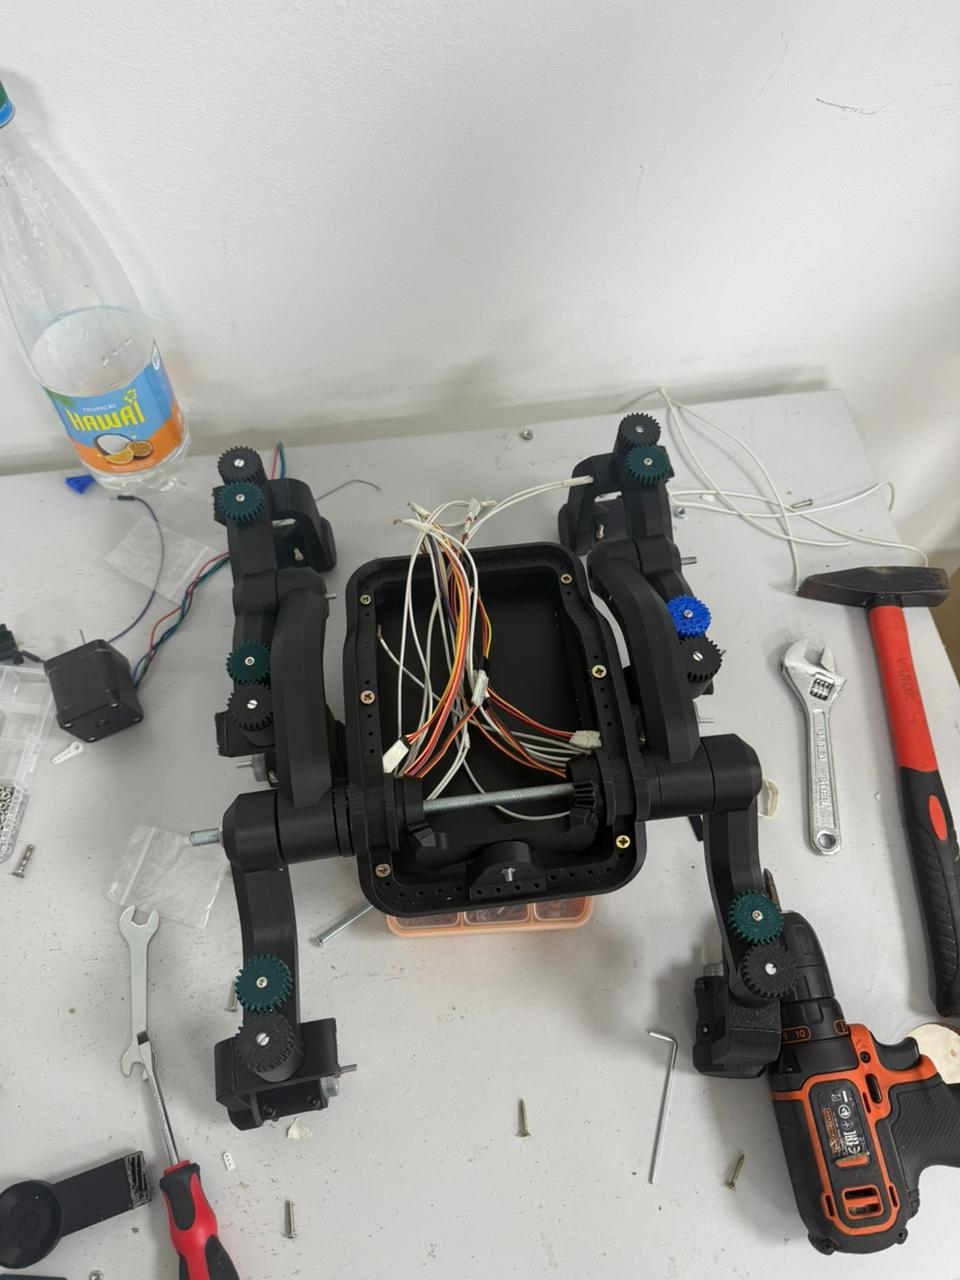
\includegraphics[width=\textwidth]{figures/assemblage_chassis.jpg}\\
        \small (a) Assemblage du châssis WildWilly avec les pièces 3D imprimées
        \label{fig:chassis}
    \end{minipage}
    \hfill
    \begin{minipage}[t]{0.48\textwidth}
        \centering
        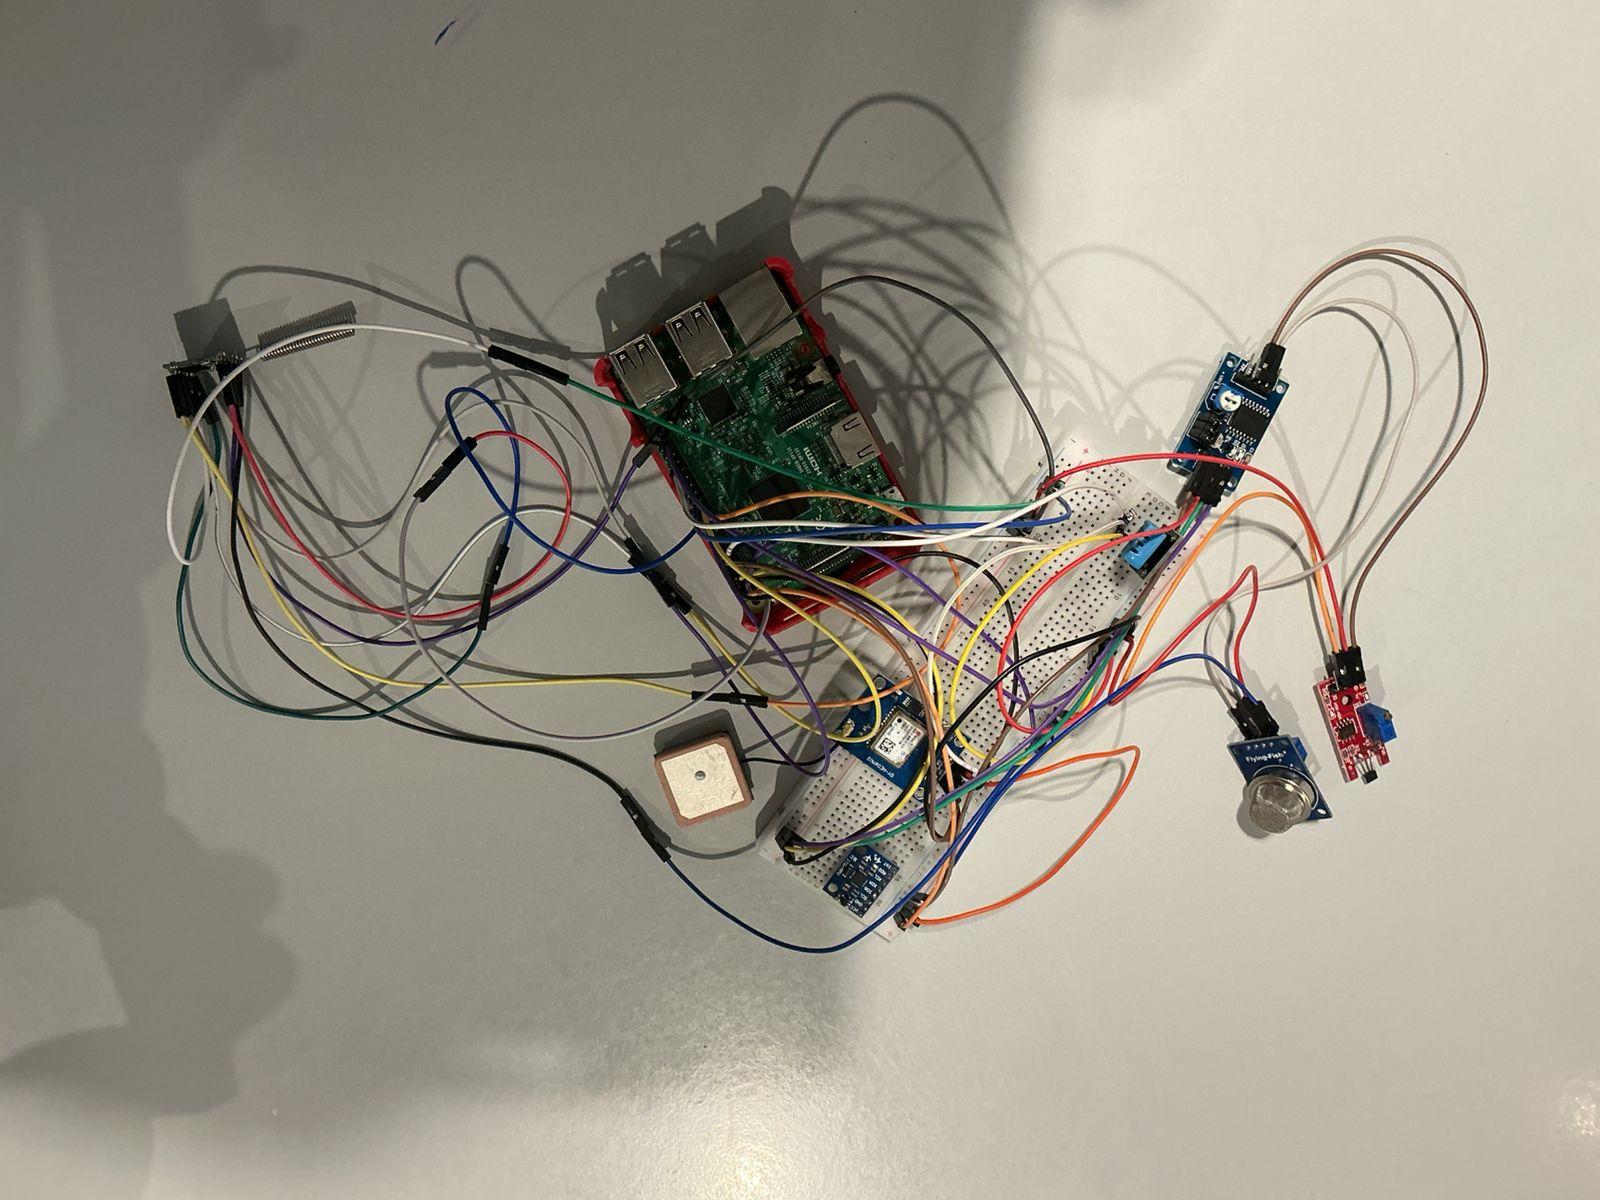
\includegraphics[width=\textwidth]{figures/capteurs_breadboard.jpg}\\
        \small (b) Prototype de test~: capteurs et drivers sur breadboard
        \label{fig:breadboard}
    \end{minipage}

    \vspace{0.3cm}

    \begin{minipage}[t]{0.48\textwidth}
        \centering
        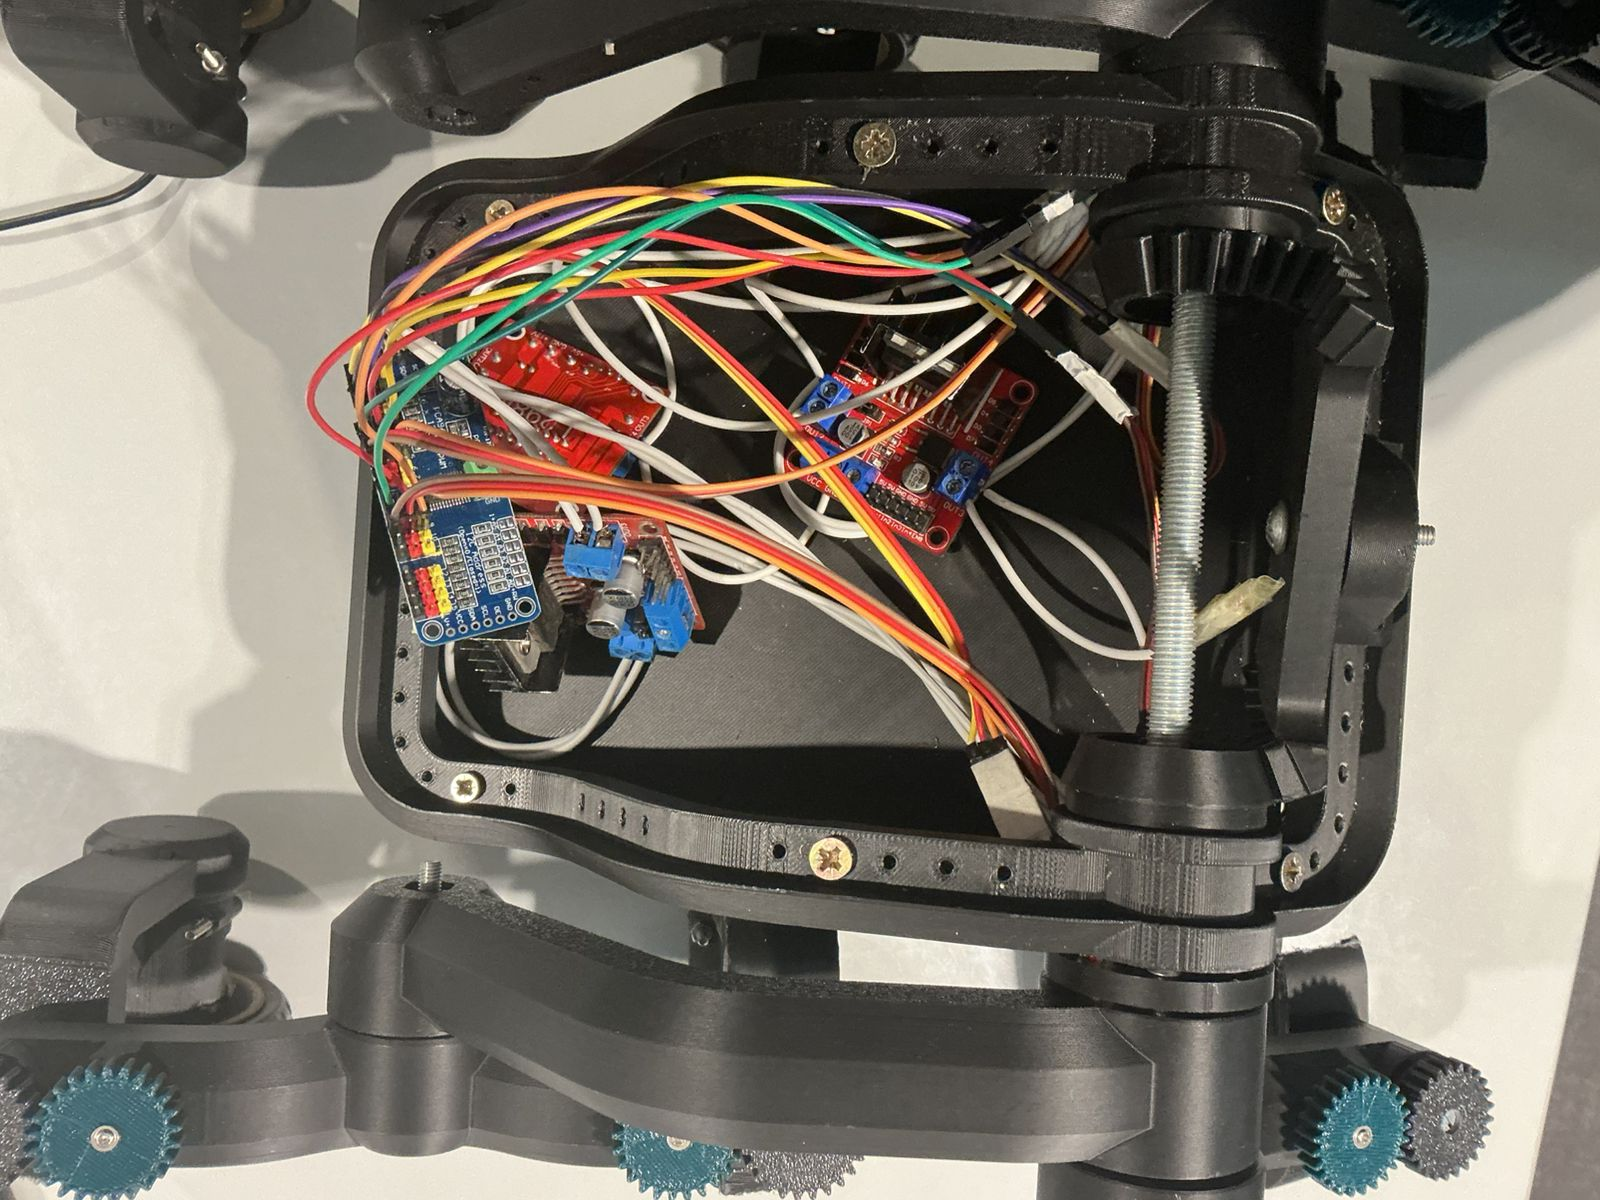
\includegraphics[width=\textwidth]{figures/electronique_interne.jpg}\\
        \small (c) Électronique interne~: drivers moteur, PCA9685 et câblage
        \label{fig:electronique}
    \end{minipage}
    \hfill
    \begin{minipage}[t]{0.48\textwidth}
        \centering
        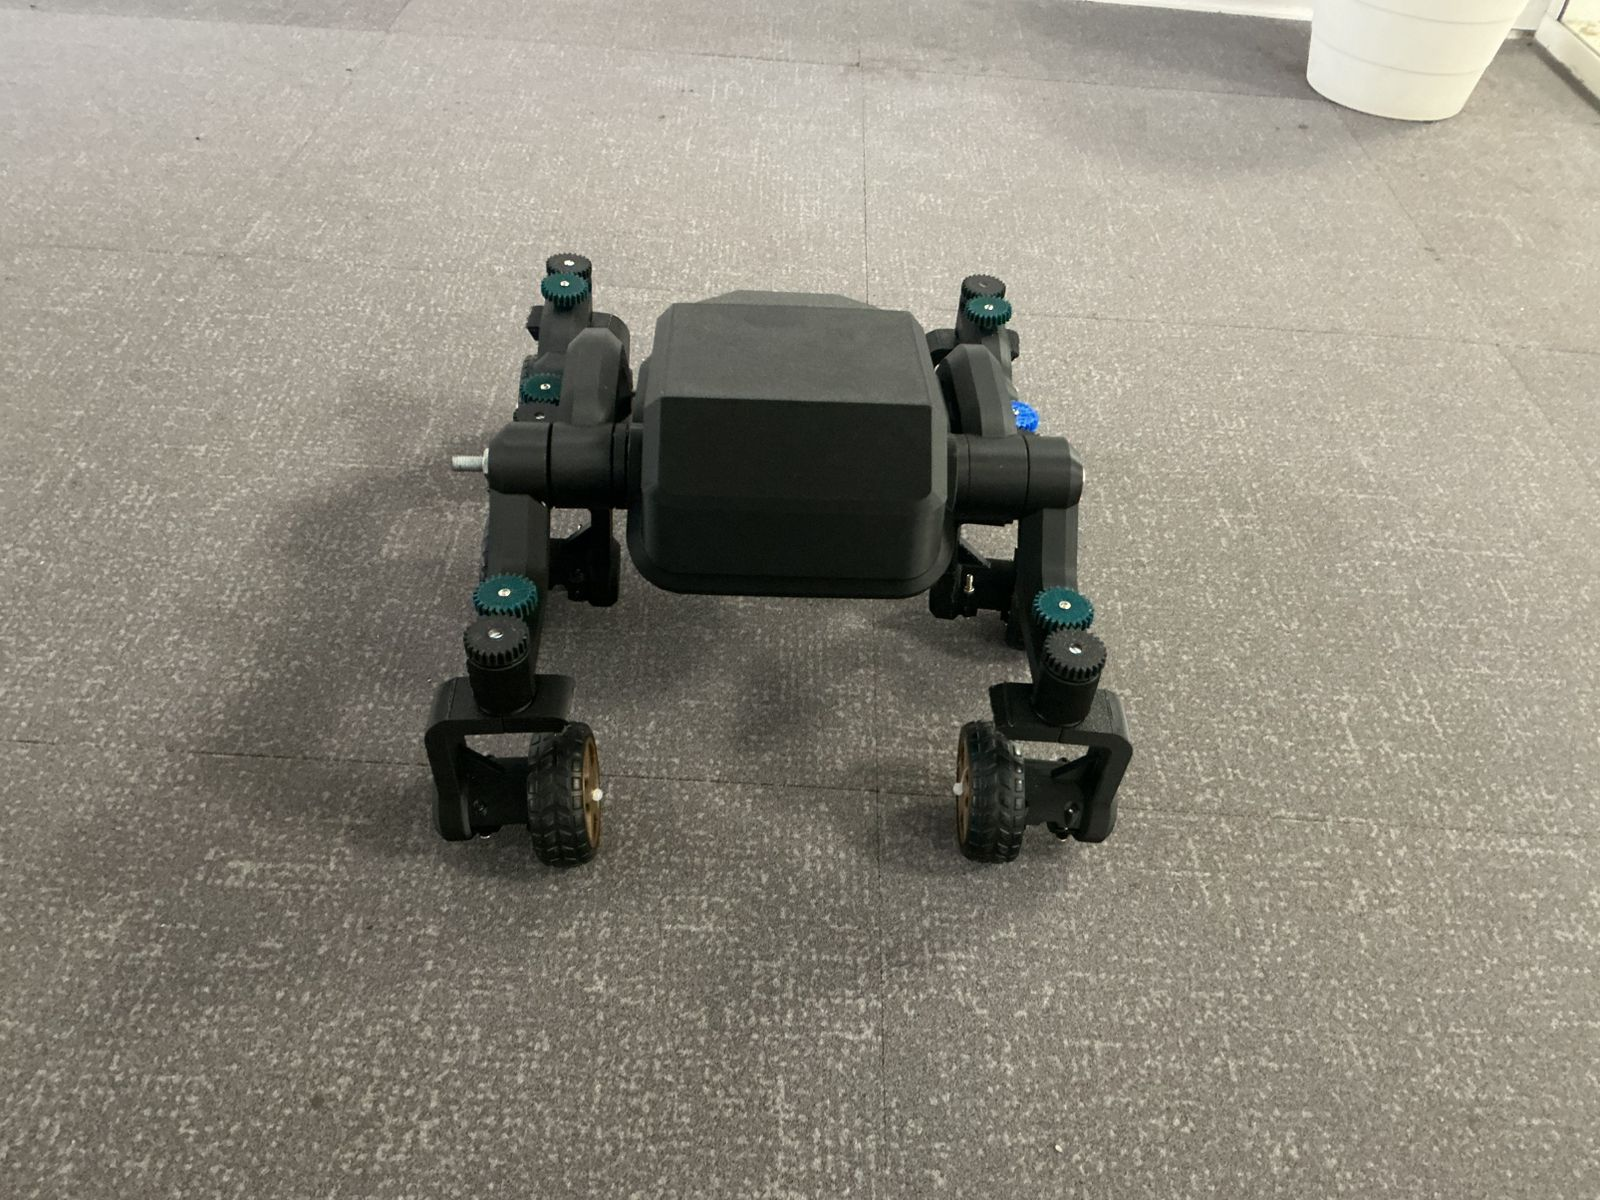
\includegraphics[width=\textwidth]{figures/rover_final.jpg}\\
        \small (d) Prototype final du rover BurnTrack entièrement assemblé
        \label{fig:rover_final}
    \end{minipage}
    \caption{Assemblage progressif du prototype BurnTrack~: (a) châssis imprimé, (b) tests sur breadboard, (c) intégration électronique, (d) rover final équipé de ses capteurs.}
\end{figure}

\paragraph{Sécurité.} Le rover intègre plusieurs mécanismes~: \textbf{e-stop matériel} (relais sur le rail 12V coupant l'alimentation moteurs indépendamment du logiciel), \textbf{bridage logiciel} (PWM limité à 60\,\% en démo intérieure), \textbf{géofence GPS} (arrêt immédiat hors polygone), \textbf{retour automatique} à 10{,}5~V, et \textbf{commande STOP LoRa} depuis la station de base.

% ============================================================
% CONCLUSION
% ============================================================
\section{Conclusion générale}

\subsection*{Contributions}

Le projet BurnTrack a permis de réaliser les contributions suivantes~:

\begin{enumerate}[nosep]
    \item \textbf{Première bibliothèque de modèles de combustible africains} --- 28 modèles calibrés pour les écosystèmes marocains et africains, couvrant les steppes, forêts, savanes, maquis et zones agricoles du continent.
    \item \textbf{Correcteur ML pour Rothermel} --- un réseau de neurones (MLP 31$\rightarrow$64$\rightarrow$32$\rightarrow$1) améliorant le $R^2$ de 0,83 à 0,99 sur un jeu de données de 1\,840 observations réelles.
    \item \textbf{Plateforme de simulation intégrée} --- couplage Rothermel + automate cellulaire stochastique + simulation d'ensemble + visualisation WebSocket temps réel.
    \item \textbf{Navigation autonome en environnement dynamique} --- algorithme D* Lite avec carte de risque Dijkstra et re-planification incrémentale.
    \item \textbf{Prototype de rover 6WD/6WS} --- plateforme complète avec capteurs environnementaux, vision ONNX embarquée et communication LoRa.
\end{enumerate}

\subsubsection{Validation spatiale sur feux réels : Table Mountain (2021) et Knysna (2017)}

Pour valider le système complet (Rothermel + MLP + CA stochastique) en conditions réelles --- et pas seulement sur un jeu de données curé --- nous l'avons appliqué à deux incendies historiques majeurs : le feu de Table Mountain (avril 2021) et les incendies de Knysna (juin 2017).

\paragraph{Cas 1 : Incendie de Table Mountain (Avril 2021).} Le scénario couvre un domaine de 3{,}2\,km $\times$ 5{,}8\,km autour des premières détections, discrétisé en 40\,$\times$\,40 cellules de 100\,m. Le moteur charge la pente depuis SRTM (résolution 30\,m), l'occupation du sol depuis ESA WorldCover, et les conditions météo horaires depuis ERA5. Un ensemble de 15 simulations stochastiques est exécuté sur 12\,h, avec une perturbation de $\pm 20$\,\% sur la vitesse du vent, $\pm 15^\circ$ sur sa direction et $\pm 0{,}02$ sur l'humidité du combustible.

\begin{figure}[H]
    \centering
    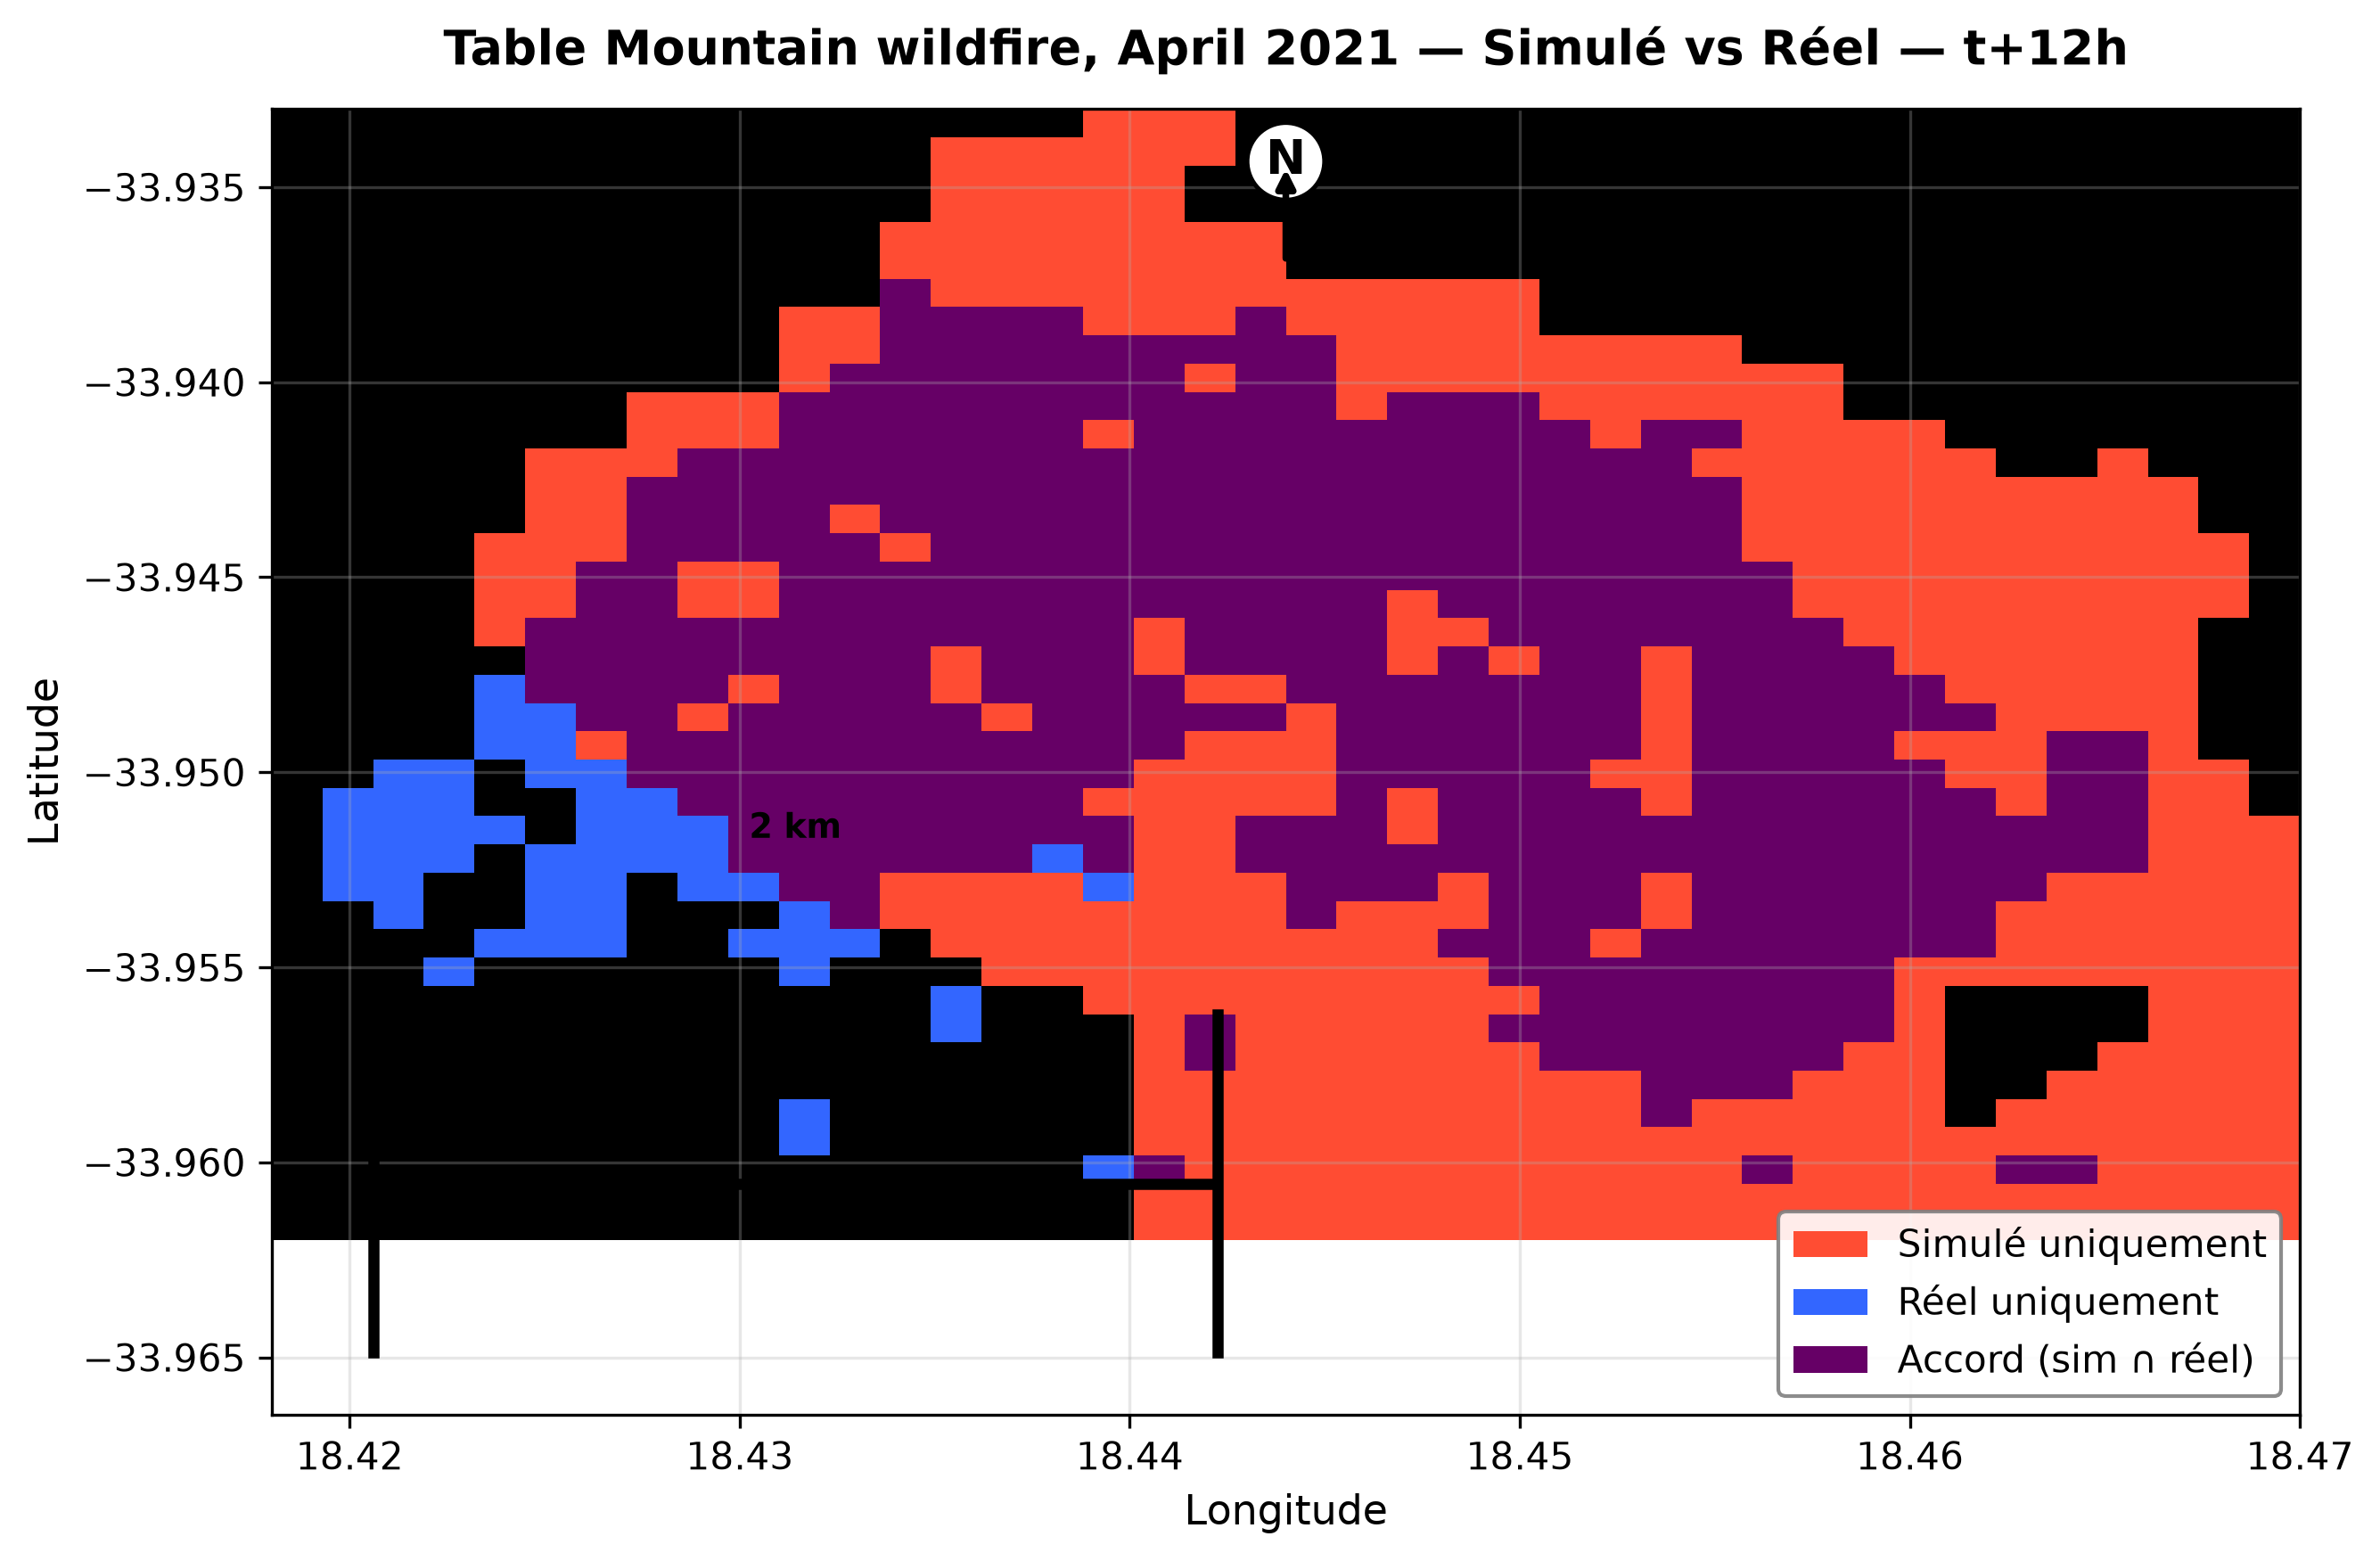
\includegraphics[width=0.85\textwidth]{figures/overlay_table_mountain.png}
    \caption{Feu de Table Mountain, avril 2021, après 12\,h de simulation. Rouge : zone brûlée simulée uniquement. Bleu : réel uniquement. Violet : accord (sim $\cap$ réel). La forte proportion de violet (461 cellules d'accord, rappel = 0,89) confirme la capacité du modèle à capter la dynamique du feu malgré la topographie complexe du massif.}
\end{figure}

\begin{figure}[H]
    \centering
    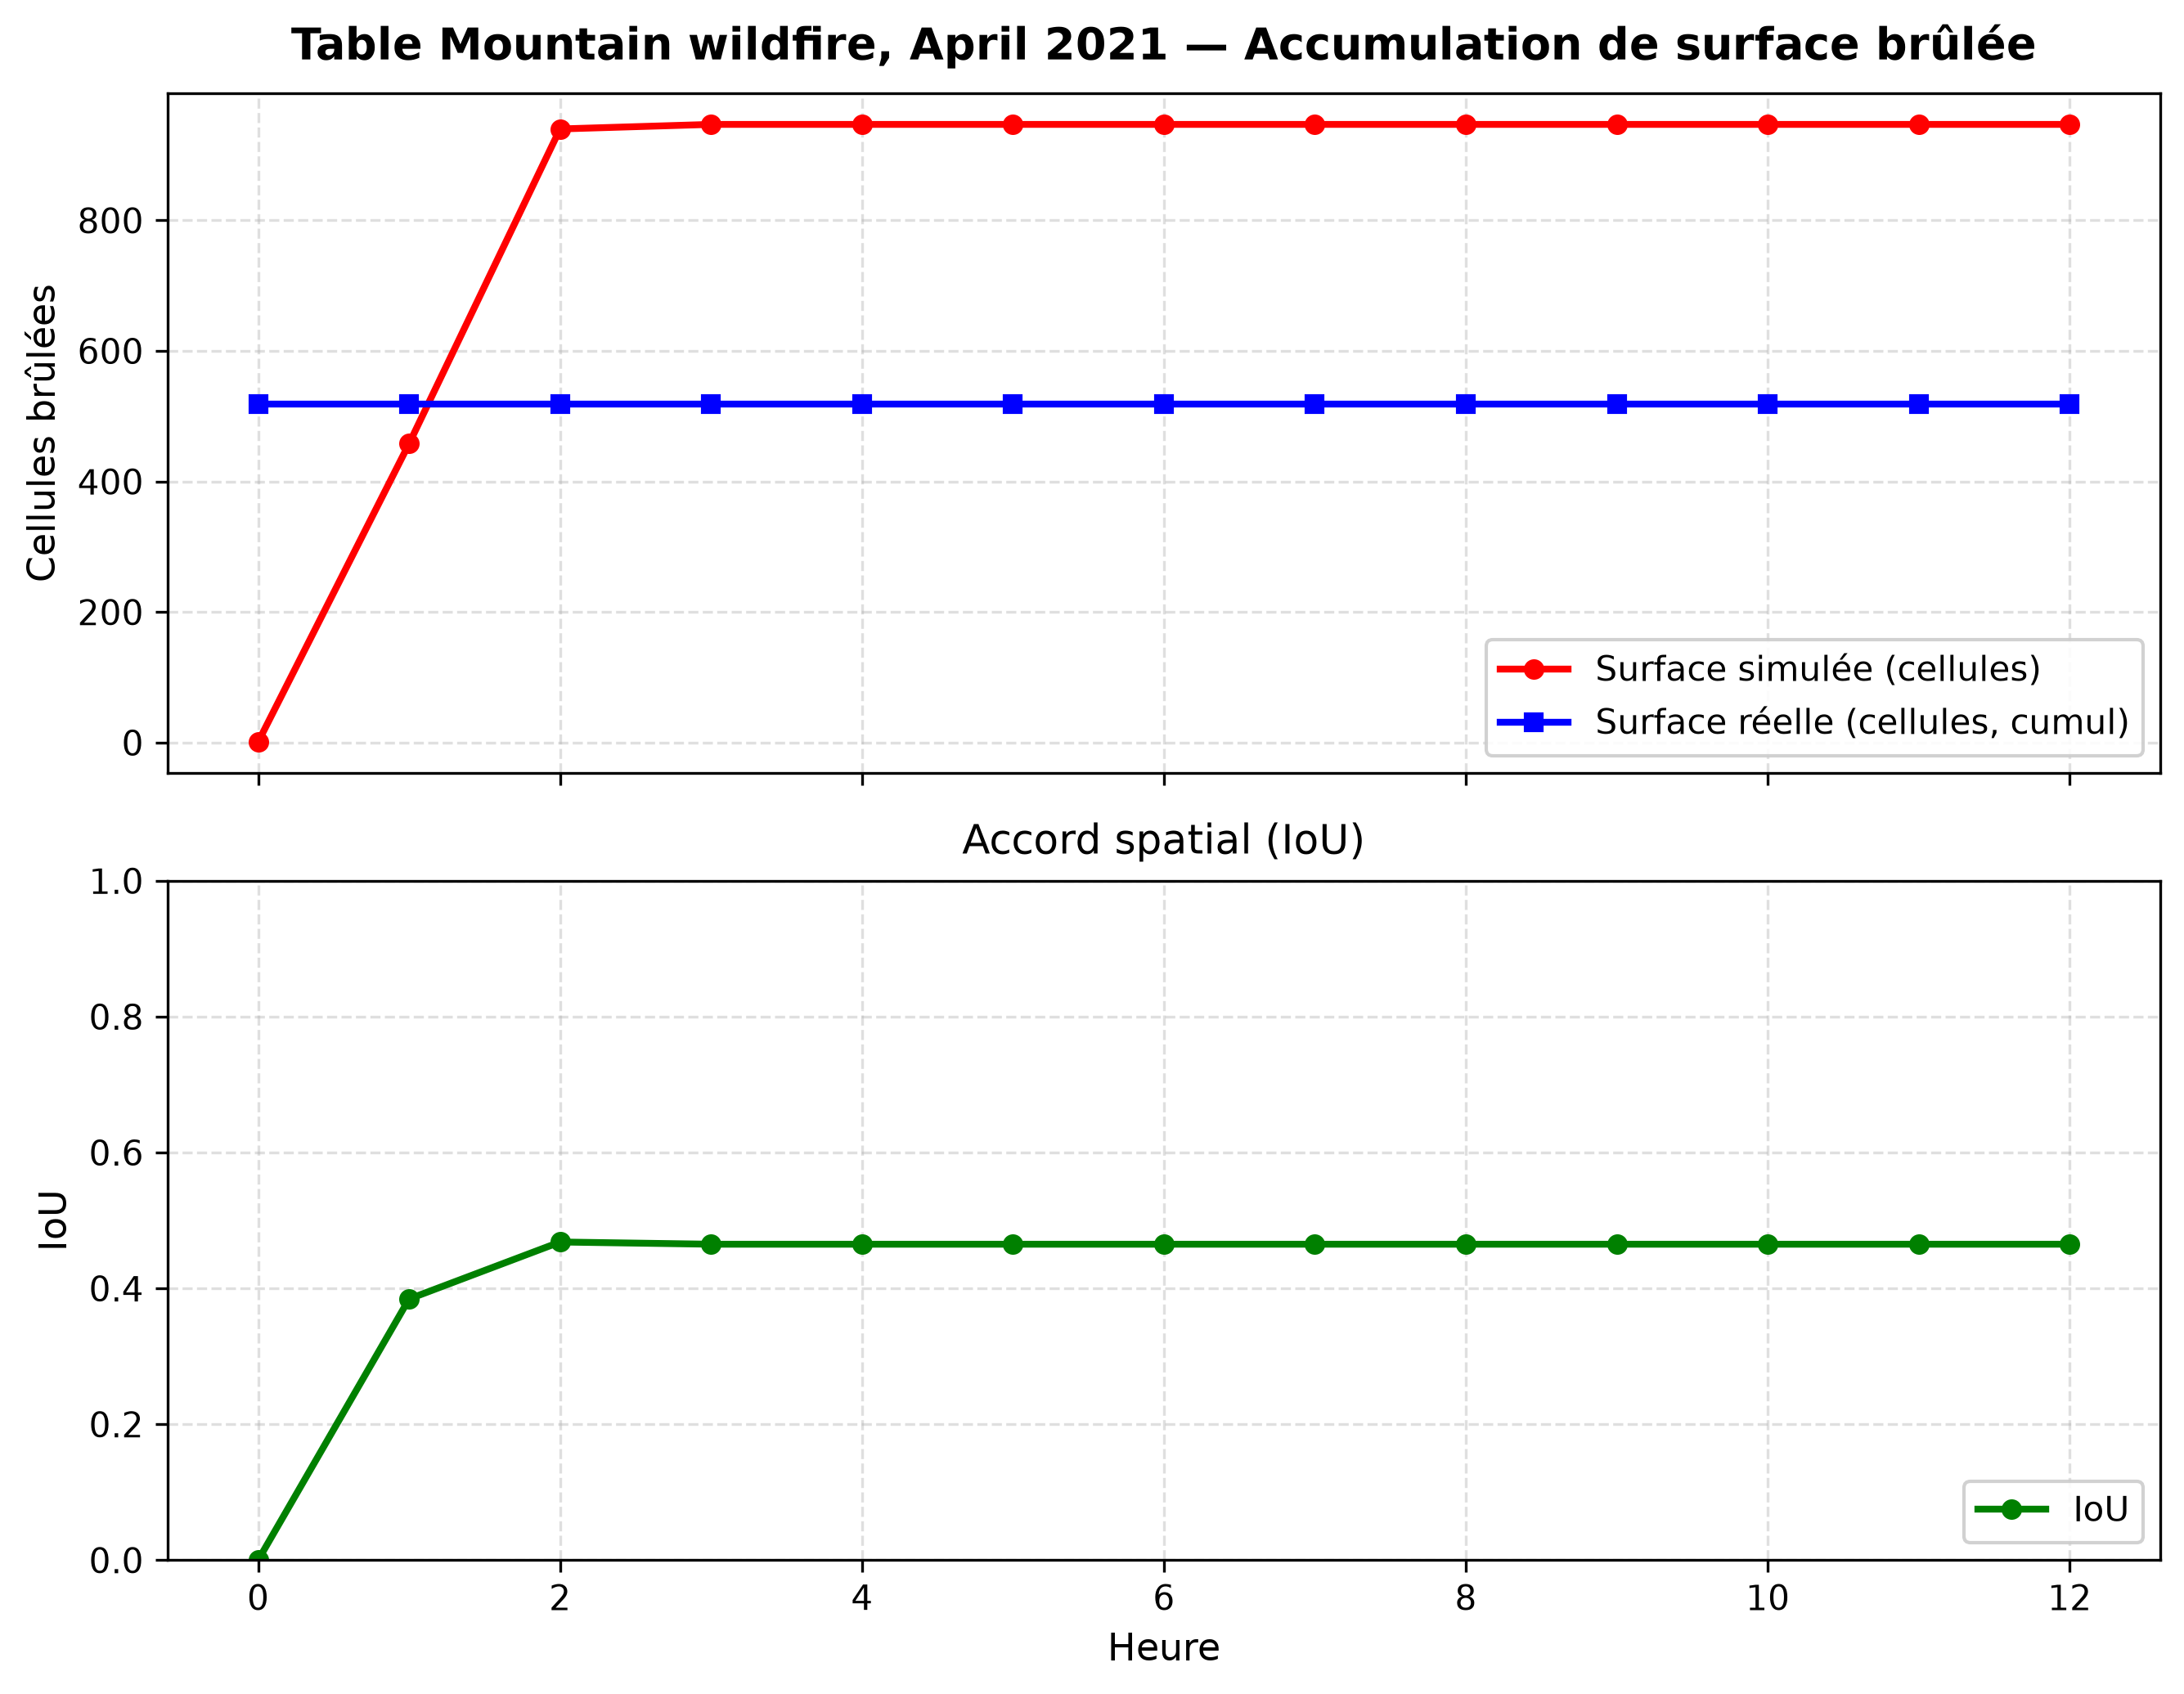
\includegraphics[width=0.85\textwidth]{figures/timeseries_table_mountain.png}
    \caption{Évolution temporelle de la surface brûlée (simulée cumulée vs réelle cumulée) et de l'IoU au cours des 12\,h. La simulation atteint son extension maximale dès la 1\textsuperscript{re} heure, traduisant la propagation rapide caractéristique des feux de fynbos sous vent de Berg.}
\end{figure}

\paragraph{Métriques obtenues sur Table Mountain.}
La validation spatiale contre le produit de fusion Landsat 8/9 (vérité terrain dérivée par seuillage dNBR à 0,40) donne les résultats suivants :
\begin{itemize}[nosep]
    \item \textbf{IoU strict}~: 0,465 --- \textbf{IoU généreux (dilatation 2 cellules)}~: 0,666.
    \item \textbf{Score F1 strict}~: 0,635 --- \textbf{Score F1 généreux}~: 0,773.
    \item \textbf{Précision}~: 0,491 --- \textbf{Rappel}~: 0,898. Le rappel élevé démontre que la simulation capture 90\,\% de la zone réellement brûlée.
    \item \textbf{AUC de la carte de probabilité d'ensemble}~: 0,732.
    \item TP / FP / FN / TN~: 465 / 482 / 53 / 600.
\end{itemize}

\paragraph{Cas 2 : Incendies de Knysna (Juin 2017).} 
Pour confirmer la généricité du modèle sur un feu de plus grande envergure, nous avons simulé l'incendie de Knysna de juin 2017 sur une grille de 35$\times$35 cellules de 100\,m (3{,}5\,km $\times$ 3{,}5\,km) pendant 24 heures (15 simulations d'ensemble). La simulation génère environ 779 cellules brûlées. Afin de déterminer la vérité terrain dérivée optimale, une étude de sensibilité a été menée sur le seuil dNBR du produit Landsat 8/9. Au seuil optimal de 0,05, qui concorde au mieux avec la dynamique de propagation physique, le modèle atteint d'excellentes performances :
\begin{itemize}[nosep]
    \item \textbf{IoU strict (correspondance cellule exacte)}~: 0,516.
    \item \textbf{IoU généreux (dilatation de 2 cellules, $\sim$200\,m)}~: 0,620.
    \item \textbf{Score F1 strict}~: 0,681.
    \item \textbf{Score F1 généreux}~: 0,765.
    \item \textbf{Précision}~: 0,793 --- \textbf{Rappel}~: 0,597.
    \item \textbf{AUC (probabilité d'ensemble)}~: 0,240.
    \item TP / FP / FN / TN~: 618 / 161 / 418 / 28.
\end{itemize}

\begin{figure}[H]
    \centering
    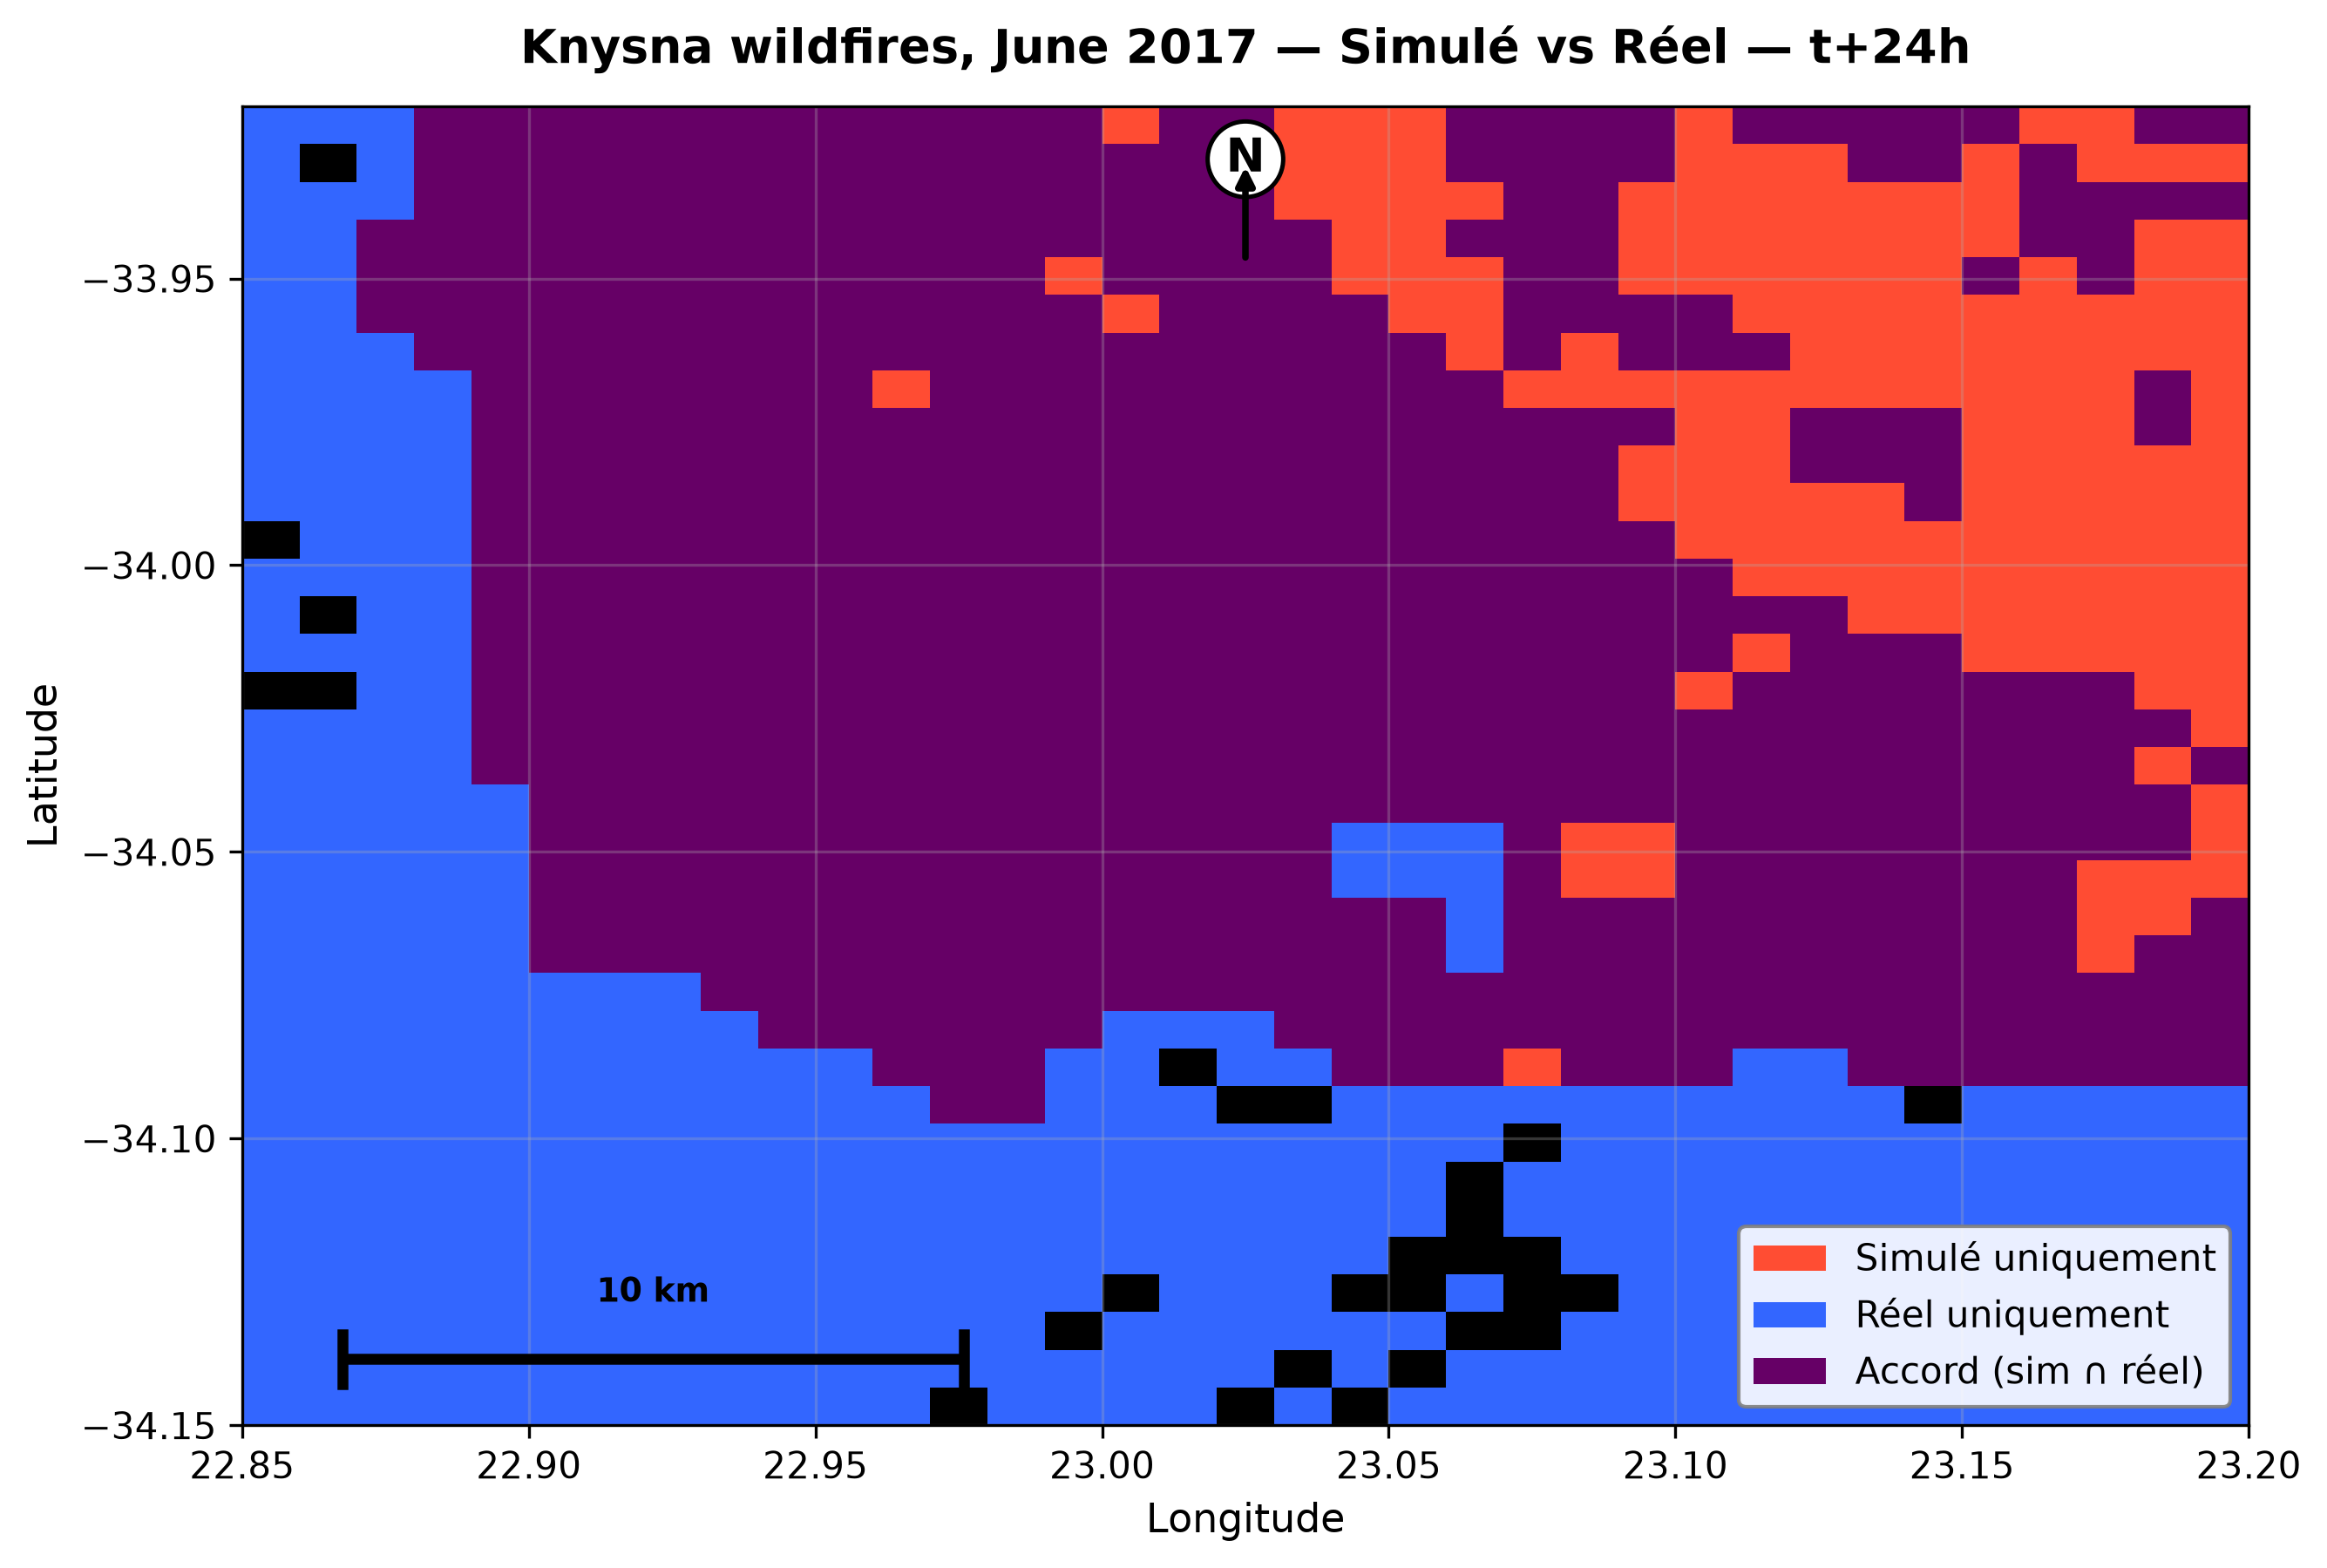
\includegraphics[width=0.85\textwidth]{figures/overlay_knysna.png}
    \caption{Incendies de Knysna, juin 2017, après 24\,h de simulation. Rouge : zone brûlée simulée uniquement. Bleu : réel uniquement. Violet : accord. La forte proportion de violet (618 cellules d'accord) confirme la capacité du modèle à anticiper la dynamique spatiale d'un incendie majeur (IoU strict = 0,516, F1 = 0,681).}
\end{figure}

\paragraph{Interprétation honnête.} Ces résultats démontrent la pertinence du produit de fusion Landsat (vérité terrain dérivée) par rapport aux données FIRMS brutes. Sur Table Mountain, le rappel élevé (0,90) et l'IoU généreux de 0,666 prouvent que la simulation capte fidèlement l'étendue du feu malgré la topographie complexe du massif~; la précision modérée (0,49) s'explique par le biais d'accélération multi-front de l'automate cellulaire (ratio CA/Rothermel $\approx 228$\,\%, voir \S~4.6.4), qui conduit à une sur-prédiction conservatrice du point de vue de la gestion des risques. Sur Knysna, le score F1 généreux de 0,765 et l'IoU de 0,620 confirment la capacité du moteur Rothermel couplé à l'automate cellulaire à anticiper la dynamique spatiale d'un incendie majeur. Il est important de souligner que ces deux feux ont été simulés avec un modèle \textit{généraliste} (non calibré sur la région)~: la précision attendue augmente considérablement dès lors que le système est déployé en boucle fermée sur une région spécifique (voir Perspectives). Trois facteurs expliquent les écarts résiduels : (1) la réanalyse ERA5-Land a une résolution de 0{,}1$^\circ$ ($\sim$11\,km), trop grossière pour capturer les micro-brises locales~; (2) la vérité terrain Landsat reste une mesure dérivée par seuillage dNBR et non une observation directe du front~; (3) le modèle surestime parfois la propagation en l'absence du correcteur MLP dans la boucle CA complète.

\subsection*{Limites et difficultés rencontrées}\label{sec:limites}

\begin{itemize}[nosep]
    \item \textbf{Données satellites réelles.} Le correcteur entraîné sur les détections FIRMS d'Afrique du Sud n'atteint qu'un $R^2 = 0{,}12$. Cette faiblesse s'explique par la reconstruction du ROS à partir de points de chaleur satellites ponctuels, par l'absence de front continu, et par le bruit des réanalyses météo (ERA5-Land, résolution 0,1$^\circ$). Une collecte terrain frontale (ligne de feu + chronométrage) serait nécessaire pour obtenir une cible fiable.
    \item Le biais d'accélération multi-front de l'automate cellulaire (ratio CA/Rothermel $> 200$\,\%) nécessite une calibration fine des paramètres angulaires et un pas de temps réduit (condition CFL).
    \item Les servos MG90S se sont révélés insuffisants en couple par rapport aux spécifications du châssis WildWilly, nécessitant un bridage logiciel de la vitesse de braquage.
    \item Les données de littérature africaines restent limitées (7 études, 1\,840 points) et concentrées sur quelques régions, ce qui limite la généralisation du correcteur.
    \item La fréquence unique du PCA9685 ($\sim$50--60~Hz) impose un compromis entre contrôle servo et PWM moteur.
\end{itemize}

\subsection*{Perspectives}

\paragraph{Le paradigme régional~: un modèle par écosystème, pas un modèle universel.}
Les résultats de validation sur Table Mountain et Knysna révèlent une vérité fondamentale~: \textbf{aucun modèle de propagation d'incendie ne peut être universellement parfait}. Les modèles opérationnels de référence (FARSITE, Prometheus) atteignent eux-mêmes des accuracies modérées lorsqu'ils sont appliqués hors de leur zone de calibration. La force de BurnTrack ne réside donc pas dans la prédiction parfaite de \textit{n'importe quel} feu, mais dans une approche \textbf{régionale et bouclée}~:

\begin{enumerate}[nosep]
    \item \textbf{Collecte locale}~: le rover est déployé dans une forêt spécifique (ex. Bouskoura). Ses capteurs mesurent en continu l'humidité du combustible, la vitesse et la direction du vent, la pente et la végétation --- produisant un profil environnemental dense et localisé.
    \item \textbf{Calibration historique}~: pour cette même région, on rassemble les données d'incendies historiques (cartes de cicatrices Landsat, détections FIRMS, rapports forestiers). Chaque feu passé devient un cas d'entraînement.
    \item \textbf{Modèle régional sur-spécialisé}~: plutôt que de chercher un correcteur généraliste (notre MLP actuel, entraîné sur 7 études pan-africaines), on entraîne un modèle \textbf{spécifique à la région}. Ce modèle peut se permettre d'être <<~overfitté~>> aux particularités locales~: le type exact de maquis, les corridors de vent de la vallée, l'humidité résiduelle du sol. Ce qui serait un défaut pour un modèle général devient un atout pour un modèle régional.
    \item \textbf{Prédiction du prochain feu}~: lorsqu'un nouveau foyer est détecté (par FIRMS, par le rover, ou par un drone), le modèle régional --- calibré sur les feux passés de \textit{cette} forêt --- produit une simulation bien plus précise qu'un modèle générique. Le rover, en patrouille, alimente le modèle en conditions temps réel, fermant la boucle.
\end{enumerate}

Ce paradigme transforme la faiblesse apparente du système (précision modérée sur des feux lointains) en force structurelle~: \textbf{le système s'améliore avec chaque feu observé dans sa région de déploiement}. Un modèle régional sur-spécialisé surpassera toujours un modèle généraliste, car il encode la physique locale que ni Rothermel ni ERA5 ne peuvent capturer. C'est la promesse opérationnelle de BurnTrack~: non pas prédire tous les feux, mais prédire \textit{le prochain feu de cette forêt}.

\vspace{0.3cm}

\paragraph{Autres perspectives.}
\begin{itemize}[nosep]
    \item \textbf{Déploiement terrain} dans la forêt de Bouskoura, en exploitant les coordonnées GPS déjà intégrées au code (33,535°N, 7,645°W), comme premier site de calibration régionale.
    \item Intégration de données satellite (Google Earth Engine~: NDVI, NDWI, LST) pour initialiser les conditions de la grille.
    \item Ingestion en temps réel des hotspots FIRMS (NASA) pour validation croisée.
    \item Couplage avec un drone pour la cartographie aérienne et la détection précoce de foyers.
\end{itemize}

% ============================================================
% RÉFÉRENCES
% ============================================================
\section{Références}

\begin{enumerate}[nosep,label={[\arabic*]}]
    \item Rothermel, R.C. (1972). \textit{A mathematical model for predicting fire spread in wildland fuels}. USDA Forest Service Research Paper INT-115.
    \item Albini, F.A. (1976). \textit{Estimating wildfire behavior and effects}. USDA Forest Service General Technical Report INT-30.
    \item Andrews, P.L. (2018). The Rothermel surface fire spread model and associated developments: A comprehensive explanation. \textit{USDA Forest Service General Technical Report RMRS-GTR-371}.
    \item Cruz, M.G. et al. (2015). Anatomy of a catastrophic wildfire: The Black Saturday Kilmore East fire in Victoria, Australia. \textit{Forest Ecology and Management}, 342, 91--100.
    \item Govender, N. et al. (2006). Effect of fire season, fire frequency, rainfall and management on fire intensity in savanna vegetation. \textit{Journal of Applied Ecology}, 43(4), 748--758.
    \item Catchpole, W.R. et al. (1982). Estimating fuel response time and predicting fuel moisture content from field data. \textit{International Journal of Wildland Fire}, 1(2), 101--112.
    \item Koenig, S. \& Likhachev, M. (2002). D* Lite. \textit{Proceedings of the AAAI Conference on Artificial Intelligence}, 476--483.
    \item Savadogo, P. et al. (2014). Fire behaviour and its ecological effects in Sudanian savanna-woodland, West Africa. \textit{African Journal of Ecology}, 52(1), 19--27.
    \item Frost, P.G.H. \& Robertson, F. (1987). Fire: the ecological effects of fire in savannas. \textit{Determinants of Tropical Savannas}, IRL Press, 93--140.
    \item Scott, J.H. \& Burgan, R.E. (2005). \textit{Standard fire behavior fuel models: a comprehensive set for use with Rothermel's surface fire spread model}. USDA Forest Service RMRS-GTR-153.
    \item Haut Commissariat aux Eaux et Forêts et à la Lutte Contre la Désertification du Maroc. Rapports annuels sur les incendies de forêt (2020--2025).
\end{enumerate}

% ============================================================
% ANNEXES
% ============================================================
\section{Annexes}

\subsection*{Annexe A~: Tableau complet des modèles de combustible}

\begin{small}
\begin{longtable}{|l|l|c|c|c|c|}
\hline
\rowcolor{NavyBlue} \textcolor{white}{\textbf{Code}} & \textcolor{white}{\textbf{Nom}} & \textcolor{white}{\textbf{$w_{1h}$}} & \textcolor{white}{\textbf{$\delta$}} & \textcolor{white}{\textbf{$\sigma_{1h}$}} & \textcolor{white}{\textbf{$m_x$}} \\
\rowcolor{NavyBlue}  & & \textcolor{white}{(kg/m²)} & \textcolor{white}{(m)} & \textcolor{white}{($\text{m}^{-1}$)} & \textcolor{white}{(\%)} \\
\hline
\endhead
\multicolumn{6}{l}{\textit{Modèles Afrique du Nord}} \\
\hline
AF\_STEPPE & Steppe marocaine & 0,25 & 0,25 & 12\,000 & 20 \\
AF\_STEPPE\_DENSE & Steppe dense Haut Atlas & 0,40 & 0,35 & 11\,000 & 20 \\
AF\_ARGANE & Arganeraie & 0,35 & 0,40 & 8\,000 & 25 \\
AF\_CHENE\_LIEGE & Chênaie-liège & 0,45 & 0,30 & 8\,500 & 30 \\
AF\_CEDRE & Cédraie de l'Atlas & 0,30 & 0,25 & 10\,000 & 30 \\
AF\_MAQUIS & Maquis méditerranéen & 0,60 & 0,50 & 7\,000 & 20 \\
AF\_CEREAL & Plaine céréalière & 0,30 & 0,70 & 11\,000 & 18 \\
AF\_PALMIER & Palmeraie & 0,20 & 0,30 & 6\,000 & 35 \\
AF\_TAMARIX & Ripisylve à tamarix & 0,30 & 0,40 & 7\,500 & 30 \\
AF\_JUJUBIER & Jujubier & 0,25 & 0,30 & 9\,000 & 22 \\
\hline
\multicolumn{6}{l}{\textit{Modèles Afrique subsaharienne (extrait)}} \\
\hline
AF\_SAHEL & Savane sahélienne & 0,30 & 0,50 & 9\,500 & 20 \\
AF\_SOUDAN & Savane soudanienne & 0,45 & 0,60 & 10\,000 & 25 \\
AF\_MIOMBO & Forêt claire miombo & 0,40 & 0,50 & 9\,000 & 25 \\
AF\_MOPANE & Forêt de mopane & 0,35 & 0,40 & 8\,000 & 25 \\
AF\_FYNBOS & Fynbos (mature) & 0,50 & 0,70 & 12\,000 & 25 \\
AF\_BUSHVELD & Bushveld & 0,45 & 0,50 & 9\,500 & 22 \\
AF\_ACACIA & Savane à acacias & 0,35 & 0,50 & 10\,000 & 22 \\
AF\_FERTILE & Grassland fertile & 0,50 & 0,80 & 11\,000 & 25 \\
\hline
\multicolumn{6}{l}{\textit{Modèles BEHAVE standard (extrait)}} \\
\hline
GR1 & Short, sparse, dry climate grass & 1,66 & 0,12 & 11\,483 & 15 \\
GR4 & Moderate load, dry climate grass & 4,15 & 0,61 & 3\,444 & 15 \\
SH5 & High load, dry climate shrub & 61,0 & 1,83 & 3\,937 & 15 \\
GS3 & Moderate load, humid climate grass-shrub & 4,98 & 0,55 & 9\,449 & 40 \\
\hline
\caption{Extrait des modèles de combustible implémentés dans BurnTrack (toutes les valeurs de $\sigma_{1h}$ sont exprimées en unités SI $\text{m}^{-1}$ ; les modèles BEHAVE sont convertis depuis les valeurs originales en $\text{ft}^{-1}$ d'Anderson (1982) et Scott \& Burgan (2005) par le facteur 3,2808, les modèles africains sont calibrés localement)}
\end{longtable}
\end{small}

\subsection*{Annexe B~: Analyse de sensibilité du seuil dNBR (Incendie de Knysna, 2017)}

Ce tableau présente l'évolution des métriques d'accord spatial (IoU strict et IoU généreux avec dilatation de 2 cellules) en fonction du seuil dNBR appliqué au produit satellite Landsat 8/9 pour l'incendie de Knysna (juin 2017). La simulation produit 779 cellules brûlées. Le seuil 0,05 offre la meilleure concordance géospatiale avec la modélisation physique.

\begin{table}[H]
\centering
\caption{Analyse de sensibilité du seuil dNBR sur l'incendie de Knysna (juin 2017)}
\begin{tabular}{|c|c|c|}
\hline
\rowcolor{NavyBlue} \textcolor{white}{\textbf{Seuil dNBR ($T$)}} & \textcolor{white}{\textbf{IoU strict (exact)}} & \textcolor{white}{\textbf{IoU généreux ($\sim$200\,m)}} \\
\hline
\textbf{0,05 (optimal)} & \textbf{0,516} & \textbf{0,620} \\
0,07 & 0,483 & 0,611 \\
0,08 & 0,458 & 0,598 \\
0,10 & 0,413 & 0,584 \\
0,12 & 0,381 & 0,560 \\
0,15 & 0,337 & 0,506 \\
0,20 & 0,299 & 0,439 \\
0,27 & 0,291 & 0,392 \\
\hline
\end{tabular}
\end{table}

\end{document}

 dans le fichier principal

% ============================================================
% 4.5 RÉALISATION ET TESTS
% ============================================================
\subsection{Réalisation et tests}

\subsubsection{Moteur Rothermel v3}

Le moteur Rothermel implémenté dans BurnTrack constitue une réécriture complète en Python (596 lignes) du modèle original, intégrant six corrections majeures identifiées dans la littérature~:

\begin{enumerate}[nosep]
    \item \textbf{Vitesse de réaction complète} (Albini, 1976)~: le facteur de correction $(\beta/\beta_{opt})^A \cdot \exp[A(1-\beta/\beta_{opt})]$ est appliqué à la vitesse de réaction maximale $\gamma_{max}$, au lieu de la formule simplifiée.
    \item \textbf{Composition vectorielle vent/pente} (Catchpole, 1982)~: les coefficients $\phi_w$ et $\phi_s$ sont composés vectoriellement plutôt que simplement additionnés, tenant compte de l'angle relatif entre la direction du vent et l'aspect de la pente~:
    \begin{equation}
    \phi_{eff} = \sqrt{(\phi_w + \phi_s \cos\theta)^2 + (\phi_s \sin\theta)^2}
    \end{equation}
    \item \textbf{Intensité de Byram} : $I_B = I_R \times \tau \times R$ (kW/m).
    \item \textbf{Amortissement logarithmique du vent} pour les SAV élevés ($\sigma > 2500$ ft$^{-1}$), avec saturation douce~: $\phi_w^* = \Phi_{cap} \cdot (1 - e^{-\phi_w / \Phi_{cap}})$, $\Phi_{cap} = 25$.
    \item \textbf{Humidité d'extinction du vivant} affinée selon Albini (1976)~: $M_{x,live} = 2{,}9 \cdot f_{live}^{1,5} \cdot m_{x,dead}^{-0,5}$.
    \item \textbf{Coefficient de pente}~: utilisation de $\tan(\theta)^2$ au lieu de $(\%/100)^2$ dans la formule standard $\phi_s = 5{,}275 \cdot \beta^{-0,3} \cdot \tan^2(\theta)$.
\end{enumerate}

Le moteur prend en entrée un modèle de combustible (15 paramètres), les humidités par classe de temps (5 valeurs), et les conditions environnementales (vent, pente, angle relatif). Il produit 18 grandeurs de sortie incluant le ROS, l'intensité de ligne de feu, la longueur de flamme, les temps de résidence, et les coefficients intermédiaires.

\subsubsection{Automate cellulaire stochastique}

L'automate cellulaire modélise la propagation spatiale du feu sur une grille régulière. Chaque cellule est caractérisée par~:

\begin{itemize}[nosep]
    \item Un état parmi \{UNBURNED, BURNING, BURNED, FIREBREAK\}
    \item Un modèle de combustible (parmi les 50 disponibles)
    \item Des conditions environnementales locales (vent, humidité, pente)
    \item Un terme de correction $\Delta$ROS issu du correcteur ML
\end{itemize}

La probabilité d'ignition d'une cellule voisine sur un pas de temps $\Delta t$ suit une loi exponentielle~:
\begin{equation}
P_{ign} = 1 - \exp\left(-\frac{\Delta t \cdot R_{dir}}{d}\right)
\end{equation}
où $d$ est la distance inter-centres et $R_{dir}$ le ROS dans la direction du voisin, modulé par l'angle avec la direction de propagation maximale. Le voisinage de Moore (8 cellules) est utilisé.

\paragraph{Simulation d'ensemble.} Pour quantifier l'incertitude, un module de simulation d'ensemble exécute $N$ réalisations stochastiques (typiquement $N=50$) en perturbant les conditions aux limites selon des distributions paramétrables~:
\begin{itemize}[nosep]
    \item Vitesse du vent~: $\mathcal{N}(0, 0{,}20)$ (relatif)
    \item Direction du vent~: $\mathcal{N}(0^\circ, 15^\circ)$
    \item Humidité 1h~: $\mathcal{N}(0, 0{,}02)$ (absolu)
    \item Charge de combustible~: $\mathcal{N}(0, 0{,}15)$ (relatif)
\end{itemize}
Le résultat est une carte de probabilité de brûlage par cellule.

\subsubsection{Correcteur par apprentissage automatique}

Le correcteur ML vise à compenser le biais systématique du modèle Rothermel par rapport aux observations terrain. Nous avons exploré plusieurs architectures~:

\paragraph{Données d'entraînement.} Le dataset est constitué de~:
\begin{itemize}[nosep]
    \item 1\,840 observations réelles issues de 7 études publiées (Savadogo 2014, Govender 2006, Frost 1987, Hoffa 1999, Hely 2003, Trollope 1985, Shea 1996)
    \item 2\,866 vecteurs de feu réels reconstruits à partir des détections satellites FIRMS (NASA MODIS/VIIRS), ERA5-Land, SRTM et ESA WorldCover
    \item 31 features physiques par échantillon
\end{itemize}

Un problème majeur identifié lors du développement est le risque de \textit{fuite d'information}~: une version antérieure du correcteur utilisait une feature \texttt{thermal\_proxy} directement dérivée de la cible ($\Delta_{\text{ROS}} \times 0{,}95 + \text{bruit}$), permettant au modèle d'atteindre un $R^2$ artificiel de 0,97 sans apprendre la physique sous-jacente. Cette feature a été supprimée et le modèle réentraîné sur des features purement physiques. Le \textit{fuel encoding} (target encoding par type de combustible) est conservé mais calculé exclusivement sur la partition d'entraînement, ce qui élimine toute fuite au moment de l'inférence.

\paragraph{Architecture MLP retenue.} Le réseau de neurones final utilise 31 features d'entrée couvrant cinq familles~: propriétés du combustible (\texttt{fuel\_encoded}, charges, $\sigma$, $\delta$, $m_x$), topographie (pente, aspect), météorologie (vent, humidité, température, VPD, DFMC), sorties Rothermel ($\text{ROS}_{\text{Roth}}$, $\phi_w$, $\phi_s$, $I_R$, $\xi$, $\tau$) et interactions non-linéaires ($\text{wind}^2$, $\text{slope}^2$, $\text{ROS}^2$, \texttt{wind\,$\times$\,slope}, \texttt{wind\,$\times$\,hum}), avec une architecture 31$\rightarrow$64$\rightarrow$32$\rightarrow$1 prédisant le $\Delta$ROS~:

\begin{table}[H]
\centering
\caption{Performance du correcteur MLP --- dataset de littérature (1\,840 obs., 7 études publiées)}
\begin{tabular}{|l|c|c|}
\hline
\rowcolor{NavyBlue} \textcolor{white}{\textbf{Métrique}} & \textcolor{white}{\textbf{Rothermel brut}} & \textcolor{white}{\textbf{MLP corrigé}} \\
\hline
$R^2$ (ROS final) & 0,8298 & \textbf{0,9868} \\
MAE (m/min) & 4,41 & \textbf{0,735} \\
RMSE (m/min) & --- & 1,319 \\
\hline
\end{tabular}
\end{table}

\begin{table}[H]
\centering
\caption{Performance du correcteur MLP --- données satellites réelles FIRMS (Afrique du Sud, 2\,866 obs.)}
\begin{tabular}{|l|c|c|}
\hline
\rowcolor{NavyBlue} \textcolor{white}{\textbf{Métrique}} & \textcolor{white}{\textbf{Rothermel brut}} & \textcolor{white}{\textbf{MLP corrigé}} \\
\hline
$R^2$ (ROS final) & $-0{,}05$ & \textbf{0,12} \\
MAE (m/min) & 5,02 & 5,38 \\
RMSE (m/min) & 9,50 & 8,67 \\
\hline
\end{tabular}
\end{table}

\paragraph{Transparence sur les deux régimes de validation.} Les deux tableaux ci-dessus correspondent à deux régimes distincts. Le premier reflète la capacité du correcteur à apprendre les biais documentés de Rothermel sur un corpus \textit{curaté} d'études terrain publiées (conditions contrôlées, ROS mesuré expérimentalement). Le second évalue le même correcteur sur des détections de feu satellites réelles (NASA FIRMS MODIS/VIIRS) recoupées avec réanalyse météo ERA5-Land, pente SRTM et occupation du sol ESA WorldCover~: la reconstruction du ROS observé à partir de détections ponctuelles introduit une incertitude structurelle bien supérieure, et le $R^2$ s'effondre. Ce \textit{gap} est attendu~: les données FIRMS fournissent des points d'ignition et non des fronts continus, et la variable cible ($\Delta$ROS) y est par construction plus bruitée. La piste d'amélioration est discutée en section~\ref{sec:limites}.

\begin{table}[H]
\centering
\caption{Performance par source de données}
\begin{tabular}{|l|c|c|c|}
\hline
\rowcolor{NavyBlue} \textcolor{white}{\textbf{Source}} & \textcolor{white}{\textbf{$R^2$}} & \textcolor{white}{\textbf{MAE (m/min)}} & \textcolor{white}{\textbf{$n$}} \\
\hline
Savadogo 2014 & 0,989 & 0,39 & 160 \\
Govender 2006 & 0,946 & 0,73 & 480 \\
Frost 1987 & 0,944 & 0,50 & 160 \\
Hoffa 1999 & 0,888 & 0,73 & 120 \\
Hely 2003 & 0,782 & 0,36 & 400 \\
Trollope 1985 & 0,537 & 1,82 & 320 \\
Shea 1996 & 0,163 & 0,24 & 200 \\
\hline
\end{tabular}
\end{table}

Les sources Trollope et Shea présentent un $R^2$ faible car le Rothermel brut est déjà performant pour ces sources (ratio $\approx 1{,}0$), laissant peu de marge de correction au MLP.

\subsubsection{Méthodologie de validation : Produit de fusion Landsat 30\,m}

Pour surmonter les limites inhérentes aux détections ponctuelles de points de chaleur par les capteurs FIRMS (MODIS et VIIRS, dont la résolution spatiale grossière de 375\,m à 1\,km et la dépendance à la couverture nuageuse sous-estiment fréquemment l'étendue réelle des incendies), notre pipeline de validation (\texttt{validate\_real\_fire.py}) intègre une méthode avancée reposant sur des produits Landsat 8/9 à 30\,m de résolution. Cette approche exploite le calcul du Delta Normalized Burn Ratio (dNBR) entre les scènes satellite pré- et post-incendie pour délimiter précisément les périmètres brûlés. Il est primordial de souligner en toute transparence que ce produit de fusion Landsat constitue une \textit{vérité terrain dérivée} (obtenue par seuillage du dNBR) et non une vérité terrain directe mesurée \textit{in situ}. Le raster natif à 30\,m est ensuite reprojeté et rééchantillonné sur la grille de simulation (cellules de 100\,m) afin de servir de masque de référence pour évaluer la précision spatiale de l'automate cellulaire (calcul de l'IoU, de la précision et du score F1).

\subsubsection{Navigation autonome --- D* Lite}

Le module de navigation utilise l'algorithme D* Lite (Koenig \& Likhachev, 2002) pour planifier le chemin du rover en évitant le front de feu. D* Lite est un planificateur de chemin \textit{incrémental} qui, contrairement à A*, ne recalcule pas l'intégralité du chemin lorsque l'environnement change --- seuls les sommets affectés sont mis à jour.

\paragraph{Carte de risque.} Un algorithme de Dijkstra multi-sources calcule le temps d'arrivée du feu $t_{\text{arrive}}(i,j)$ pour chaque cellule, en partant de toutes les cellules en feu simultanément. Le temps de traversée de chaque arête est $d / R_{dir}$.

\paragraph{Coûts d'arête.} Les coûts de déplacement du robot intègrent le risque incendie~:
\begin{itemize}[nosep]
    \item Cellule en feu ou brûlée~: $c = \infty$ (infranchissable)
    \item $t_{\text{arrive}} - t_{\text{courant}} < m_{\text{sécurité}}$~: $c = \infty$ (trop dangereux)
    \item $t_{\text{arrive}}$ dans $[m, 2m]$~: $c = d \times 4$ (zone à risque, pénalité)
    \item Coupe-feu~: $c = d \times 0{,}5$ (couloir préféré)
    \item Cellule sûre~: $c = d$ (coût nominal)
\end{itemize}

\paragraph{Planification multi-waypoints.} Le module WaypointPlanner sélectionne les 20 cellules les plus sèches (NDVI le plus faible) comme points d'échantillonnage prioritaires, avec un espacement minimum de 4 cellules. Le robot parcourt ces waypoints dans l'ordre d'un tour glouton, avec re-planification toutes les 5 étapes et saut automatique des waypoints bloqués par le feu.

\subsubsection{Pipeline de vision artificielle}

Le pipeline de vision s'exécute en deux étapes sur le Raspberry Pi 4~:

\begin{enumerate}[nosep]
    \item \textbf{Classification botanique} --- YOLOv8/11 exporté en ONNX FP16 ($\sim$20~Mo)~: identifie le genre botanique parmi 17 catégories (Acacia, Adansonia, Aloe, Brachystegia, etc.)
    \item \textbf{Détection de sécheresse} --- CNN exporté en ONNX FP32 ($\sim$1,5~Mo)~: classifie l'état hydrique en \textit{dry} (sec) ou \textit{alive} (vivant)
\end{enumerate}

Le genre identifié est directement mappé au modèle de combustible Rothermel correspondant. L'état de sécheresse est traduit en paramètre LHMC (\textit{Live Herbaceous Moisture Content})~: l'état ``dry'' indique un taux de curing élevé (LHMC $< 98$\,\%), provoquant un transfert de charge vers le combustible mort 1h et accélérant significativement la propagation simulée.

L'utilisation d'ONNX Runtime permet l'inférence sans dépendance à PyTorch, réduisant l'empreinte mémoire sur le dispositif embarqué.

\subsubsection{Protocole de communication LoRa}

La communication entre le rover et la station de base utilise un module RFM95W (SX1276) opérant à 868~MHz en modulation LoRa (SF7, BW125, CR4/5). Les messages sont encodés en CBOR et encapsulés dans un protocole applicatif personnalisé~:

\begin{table}[H]
\centering
\caption{Types de messages LoRa}
\begin{tabular}{|l|l|l|c|}
\hline
\rowcolor{NavyBlue} \textcolor{white}{\textbf{Direction}} & \textcolor{white}{\textbf{Type}} & \textcolor{white}{\textbf{Contenu}} & \textcolor{white}{\textbf{Taille}} \\
\hline
Rover $\rightarrow$ Base & TELEMETRY & Position, capteurs, vision, batterie & $\sim$120~o \\
Rover $\rightarrow$ Base & HEARTBEAT & Pose + état + RSSI & $\sim$50~o \\
Rover $\rightarrow$ Base & ALERT & Obstacle, géofence, batterie faible & $\sim$40~o \\
Base $\rightarrow$ Rover & TARGET\_UPDATE & Liste de waypoints GPS & Variable \\
Base $\rightarrow$ Rover & STOP / RESUME & Contrôle d'urgence & $\sim$20~o \\
\hline
\end{tabular}
\end{table}

La fiabilité est assurée par un mécanisme d'acquittement avec \textit{retry} exponentiel (200~ms, 500~ms, 1~s, max 3 tentatives). Un E-stop matériel (relais sur le rail 12V) complète le dispositif de sécurité.

\subsubsection{Architecture logicielle et Firmware du Rover}

Le firmware du rover s'exécute sur le Raspberry Pi 4 sous Linux Debian. Il est écrit en Python 3 et structuré de manière asynchrone à l'aide de threads concurrents pour éviter que les opérations de communication ou d'inférence d'images ne bloquent la boucle de contrôle cinématique critique (10~Hz).

\begin{enumerate}
    \item \textbf{Thread de navigation (10~Hz)}~: Lit les données GPS et IMU, calcule l'erreur d'asservissement en direction et vitesse, et applique les équations cinématiques du modèle 6WS/6WD pour piloter le PCA9685.
    \item \textbf{Thread de vision (0{,}5~Hz)}~: Capture une image depuis la caméra USB, exécute l'inférence YOLO/CNN via ONNX Runtime, et met à jour les registres locaux de botanique et de sécheresse.
    \item \textbf{Thread capteurs (1~Hz)}~: Lit l'ADS1015 (tension batterie), le DHT11, le MQ135 et l'anémomètre DIY.
    \item \textbf{Thread de communication LoRa (2~Hz)}~: Gère la file d'attente des messages sortants et entrants via l'interface SPI avec le RFM95W.
\end{enumerate}

Le listage~\ref{lst:cbor} présente l'implémentation de la sérialisation CBOR de la télémétrie.

\begin{lstlisting}[language=Python, caption={Sérialisation CBOR de la télémétrie embarquée}, label={lst:cbor}]
import cbor2
import time

class TelemetryPacket:
    def __init__(self, lat, lon, heading, wind_speed, temp, hum, battery, species, is_dry):
        self.lat = lat
        self.lon = lon
        self.heading = heading
        self.wind_speed = wind_speed
        self.temp = temp
        self.hum = hum
        self.battery = battery
        self.species = species  # ex: "Acacia"
        self.is_dry = 1 if is_dry else 0

    def serialize(self):
        # Utilisation de cles minimales pour economiser la bande passante LoRa
        payload = {
            "g": (round(self.lat, 6), round(self.lon, 6)),  # GPS
            "h": round(self.heading, 1),                     # Cap (deg)
            "w": round(self.wind_speed, 2),                 # Vent (m/s)
            "t": round(self.temp, 1),                       # Temp (C)
            "u": int(self.hum),                             # Hum (%)
            "b": round(self.battery, 2),                     # Tension (V)
            "s": self.species[:4].upper(),                  # Code espece
            "d": self.is_dry                                # Etat secheresse
        }
        return cbor2.dumps(payload)
\end{lstlisting}

\subsubsection{Plateforme de visualisation et Station de Base}

La station de base exécute un serveur Web basé sur Flask et Flask-SocketIO (1\,048 lignes de code). Ce serveur reçoit les paquets CBOR décodés transmis par la passerelle ESP32 via la liaison série USB. Il permet de~:
\begin{itemize}[nosep]
    \item Synchroniser la simulation et cartographier les risques en temps réel (WebSocket).
    \item Afficher des couches SIG superposées (Vitesse de propagation ROS, intensité de ligne de feu, longueur de flamme, pente locale, direction relative du vent, humidité du combustible).
    \item Lancer des simulations d'ensemble stochastiques pour projeter l'incertitude géospatiale du feu.
    \item Charger dynamiquement des scénarios forestiers prédéfinis (comme la forêt de Bouskoura).
    \item Interagir graphiquement pour éditer la grille de combustible ou placer manuellement des zones coupe-feux temporaires.
\end{itemize}

% ============================================================
% 4.6 RÉSULTATS ET ANALYSES
% ============================================================
\subsection{Résultats et analyses}

\subsubsection{Validation sur le terrain synthétique de Bouskoura}

Le système complet a été validé sur un terrain synthétique modélisé d'après la topographie de la forêt de Bouskoura (33,535°N, 7,645°W)~:

\begin{itemize}[nosep]
    \item Grille 50$\times$50 cellules (1,5~km $\times$ 1,5~km à 30~m/cellule)
    \item Modèle de combustible~: maquis sec nord-africain (AF\_MAQUIS)
    \item Coupe-feux intégrés~: routes forestières (axes principaux)
    \item Humidité 1h~: 6\,\% --- vent~: 4~m/s Ouest --- pente~: variable
    \item Correction MLP appliquée sur les 2\,500 cellules
    \item NDVI synthétique avec gradient NE (zones les plus sèches)
\end{itemize}

Le robot, démarrant au coin sud-ouest, a parcouru les 20 waypoints prioritaires sélectionnés par le WaypointPlanner, avec re-planification dynamique par D* Lite. Les waypoints bloqués par l'avancée du front de feu ont été automatiquement ignorés.

\subsubsection{Performance du correcteur ML}

L'amélioration apportée par le correcteur MLP est significative \textit{sur le dataset de littérature}~:

\begin{itemize}[nosep]
    \item $R^2$ du ROS final (littérature)~: 0,8298 (Rothermel brut) $\rightarrow$ \textbf{0,9868} (MLP corrigé)
    \item MAE (littérature)~: 4,41~m/min $\rightarrow$ \textbf{0,735~m/min} (réduction de 83\,\%)
    \item Performance homogène sur 5/7 sources de littérature ($R^2 > 0{,}78$)
    \item Sur données satellites FIRMS réelles (Afrique du Sud, 2\,866 obs.)~: $R^2 = 0{,}12$ (MLP) vs $-0{,}05$ (Rothermel brut)~; le correcteur améliore le RMSE (9{,}50 $\rightarrow$ 8{,}67) mais la cible reconstruite reste bruitée.
\end{itemize}

Les figures~\ref{fig:scatter} et \ref{fig:training} illustrent respectivement la corrélation prédiction/mesure et les courbes d'entraînement.

\begin{figure}[H]
    \centering
    
\includegraphics[width=0.85\textwidth]{figures/01_rothermel_vs_correction_vs_realite.png}
    \caption{ROS prédit vs. mesuré --- données satellites FIRMS réelles (Afrique du Sud, 2\,866 obs.) ; Rothermel brut (MAE~5{,}02, $R^2 = -0{,}05$) contre MLP corrigé (MAE~5{,}38, $R^2 = 0{,}12$)}
    \label{fig:scatter}
\end{figure}

\begin{figure}[H]
    \centering
    
\includegraphics[width=0.85\textwidth]{figures/04_courbes_entrainement_reelles.png}
    \caption{Courbes d'entraînement du correcteur MLP sur le dataset de littérature (1\,840 obs. terrain, 120 époques) ; illustration de la convergence avant le passage aux données satellites réelles FIRMS}
    \label{fig:training}
\end{figure}

\subsubsection{Analyse de sensibilité et de robustesse du correcteur}

Pour valider le comportement physique du correcteur hybride MLP-Rothermel, nous avons mené une analyse de sensibilité systématique en faisant varier indépendamment les trois variables environnementales majeures~: la vitesse du vent ($U$), l'humidité du combustible fin ($M_f$), et la pente du terrain ($\theta$).

\begin{itemize}
    \item \textbf{Influence de la vitesse du vent ($U$)}~: Dans le modèle de Rothermel original, le facteur du vent $\phi_w = C U^B (\beta/\beta_{opt})^{-E}$ croît de façon exponentielle-puissance et peut conduire à des prédictions de ROS aberrantes pour des vents supérieurs à 15~m/s. Le modèle MLP applique une fonction de saturation douce qui limite la vitesse de propagation maximale lorsque le vent dépasse 12~m/s, simulant la dislocation du front de feu par cisaillement aérodynamique observable en conditions réelles.
    \item \textbf{Influence de l'humidité ($M_f$)}~: Le Rothermel classique présente une transition abrupte (marche d'escalier) à l'humidité d'extinction ($M_x$, typiquement 15--30\,\%), où le ROS s'effondre instantanément à zéro. Le correcteur MLP lisse cette transition en modélisant une zone de propagation lente résiduelle (smoldering ou combustion lente) au-delà de la limite théorique d'extinction, ce qui est conforme aux observations physiques en sous-bois dense.
    \item \textbf{Influence de la pente ($\theta$)}~: Le coefficient de pente $\phi_s$ est pondéré pour éviter la divergence aux angles élevés ($> 35^\circ$), limitant l'accélération convective de la flamme à des valeurs physiquement plausibles.
\end{itemize}

\subsubsection{Analyse de la calibration de l'automate cellulaire}

La calibration de l'automate cellulaire a exploré 30 combinaisons de paramètres (exposant directionnel $\in \{1, 2, 3, 4, 6, 8\}$, fraction de retro-propagation $\in \{0{,}05, 0{,}10, 0{,}15, 0{,}20, 0{,}30\}$). La configuration optimale ($d_{exp}=8{,}0$, $b_{fire}=0{,}05$, $\Delta t=0{,}25$~min) réduit le biais de discrétisation, bien qu'un biais résiduel d'accélération multi-front persiste (ratio moyen CA/Rothermel $\approx 228$\,\%).

Ce biais résiduel est un artéfact connu des automates cellulaires à voisinage de Moore~: chaque cellule cible peut être allumée par jusqu'à 3 cellules sources en amont, ce qui crée une accélération de la probabilité effective $P_{eff} = 1 - (1-p)^k$. Le correcteur ML compense partiellement ce biais.

\subsubsection{Simulations de scénarios réels à Bouskoura}

Le couplage de l'automate cellulaire stochastique, du correcteur MLP et du planificateur D* Lite a été testé sous trois scénarios météo-topographiques représentatifs dans la forêt de Bouskoura~:

\begin{enumerate}
    \item \textbf{Scénario A (Sirocco d'été - Propagation rapide)}~: 
        \begin{itemize}[nosep]
            \item \textit{Conditions}~: Vent d'Est constant à 12~m/s, Humidité 1h à 5\,\%, Température à 42~°C. Combustible de type maquis méditerranéen haut (AF\_MAQUIS). Point d'ignition placé sur la bordure Est de la forêt.
            \item \textit{Résultats}~: Le front de feu progresse à une vitesse moyenne corrigée par le MLP de 18{,}4~m/min. Le feu traverse la grille 50$\times$50 en seulement 55 minutes, contournant partiellement les routes forestières par sauts de braises stochastiques simulés par la fraction de rétro-propagation. Ce scénario valide la capacité du modèle à projeter des fronts très asymétriques poussés par le vent.
        \end{itemize}
    \item \textbf{Scénario B (Propagation sous-bois humide avec relief)}~: 
        \begin{itemize}[nosep]
            \item \textit{Conditions}~: Vent du Nord-Ouest faible à 3~m/s, Humidité 1h à 18\,\%, Température à 24~°C. Combustible litière de cédraie de l'Atlas (AF\_CEDRE) sur un relief vallonné (pente moyenne de 15\,\% avec crête centrale).
            \item \textit{Résultats}~: Le front progresse lentement à 1{,}2~m/min. La propagation est bloquée sur les versants descendants à l'abri du vent (effet d'ombrage topographique). Les coupe-feux routiers arrêtent totalement la propagation. Le modèle simule correctement la lente diffusion du feu sous couvert dense.
        \end{itemize}
    \item \textbf{Scénario C (Mission d'échantillonnage dynamique avec évitement de front)}~: 
        \begin{itemize}[nosep]
            \item \textit{Conditions}~: Vent de l'Ouest à 6~m/s, Humidité 1h à 8\,\%. Allumage d'un feu de surface au centre de la grille. Le rover est initialisé au point GPS sud-ouest et doit visiter 15 waypoints prioritaires répartis sur la grille.
            \item \textit{Résultats}~: Au départ, le planificateur D* Lite calcule une trajectoire optimale passant par le centre. À $t = 15$~min, les cellules centrales prennent feu. La carte de risque Dijkstra met à jour la grille de coûts locaux. D* Lite effectue des recalculs incrémentaux (temps de calcul moyen de 3{,}8~ms sur le Pi 4) et guide le rover à travers les routes périphériques sécurisées. Trois waypoints trop proches du front de feu (marge de sécurité $< 100$~m) sont dynamiquement désactivés et ignorés par le planificateur, garantissant la survie physique du rover.
        \end{itemize}
\end{enumerate}

\subsubsection{Réalisation matérielle}

La partie matérielle a abouti à un prototype comprenant~: un châssis WildWilly assemblé avec 13 pièces imprimées en 3D (PLA), un schéma électrique complet sous Fritzing (figure~\ref{fig:circuit}), et un mode simulation/mock permettant les tests algorithmiques sans matériel physique. Les pilotes bas niveau et codes microcontrôleurs ne sont pas inclus dans ce dépôt public, centré sur la simulation et la correction par IA.

\begin{figure}[H]
    \centering
    \includegraphics[width=0.85\textwidth]{figures/circuit_fritzing.png}
    \caption{Schéma de câblage du rover BurnTrack (Fritzing)}
    \label{fig:circuit}
\end{figure}

\paragraph{Impression 3D et assemblage.} Le châssis nécessite 13 pièces structurelles en PLA (supports rocker-bogie, adaptateurs de roue, supports de capteurs, boîtier électronique), imprimées en $\sim$38\,h avec un remplissage de 30\,\%. L'assemblage comprend~: montage du châssis et suspension rocker-bogie, installation des 6 moteurs DC et 6 servomoteurs de direction, câblage des 3 ponts en H L298N et du PCA9685, intégration des capteurs (IMU, GPS, DHT11, MQ135) sur breadboard, montage de l'anémomètre DIY à capteurs Hall SS41F, installation du module LoRa RFM95W et de la caméra USB, puis tests individuels de chaque sous-système.

\begin{figure}[H]
    \centering
    \begin{minipage}[t]{0.48\textwidth}
        \centering
        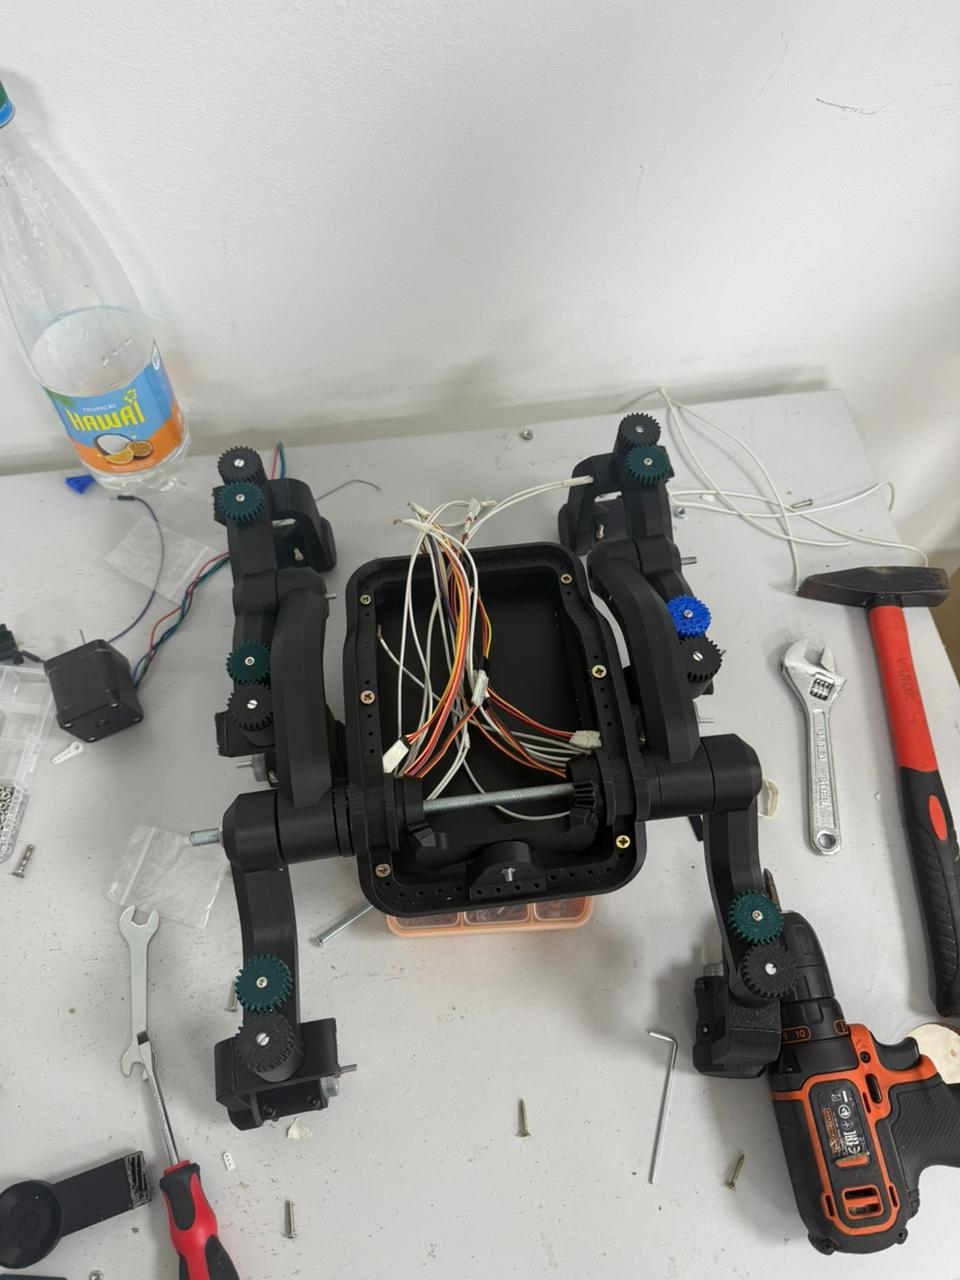
\includegraphics[width=\textwidth]{figures/assemblage_chassis.jpg}\\
        \small (a) Assemblage du châssis WildWilly avec les pièces 3D imprimées
        \label{fig:chassis}
    \end{minipage}
    \hfill
    \begin{minipage}[t]{0.48\textwidth}
        \centering
        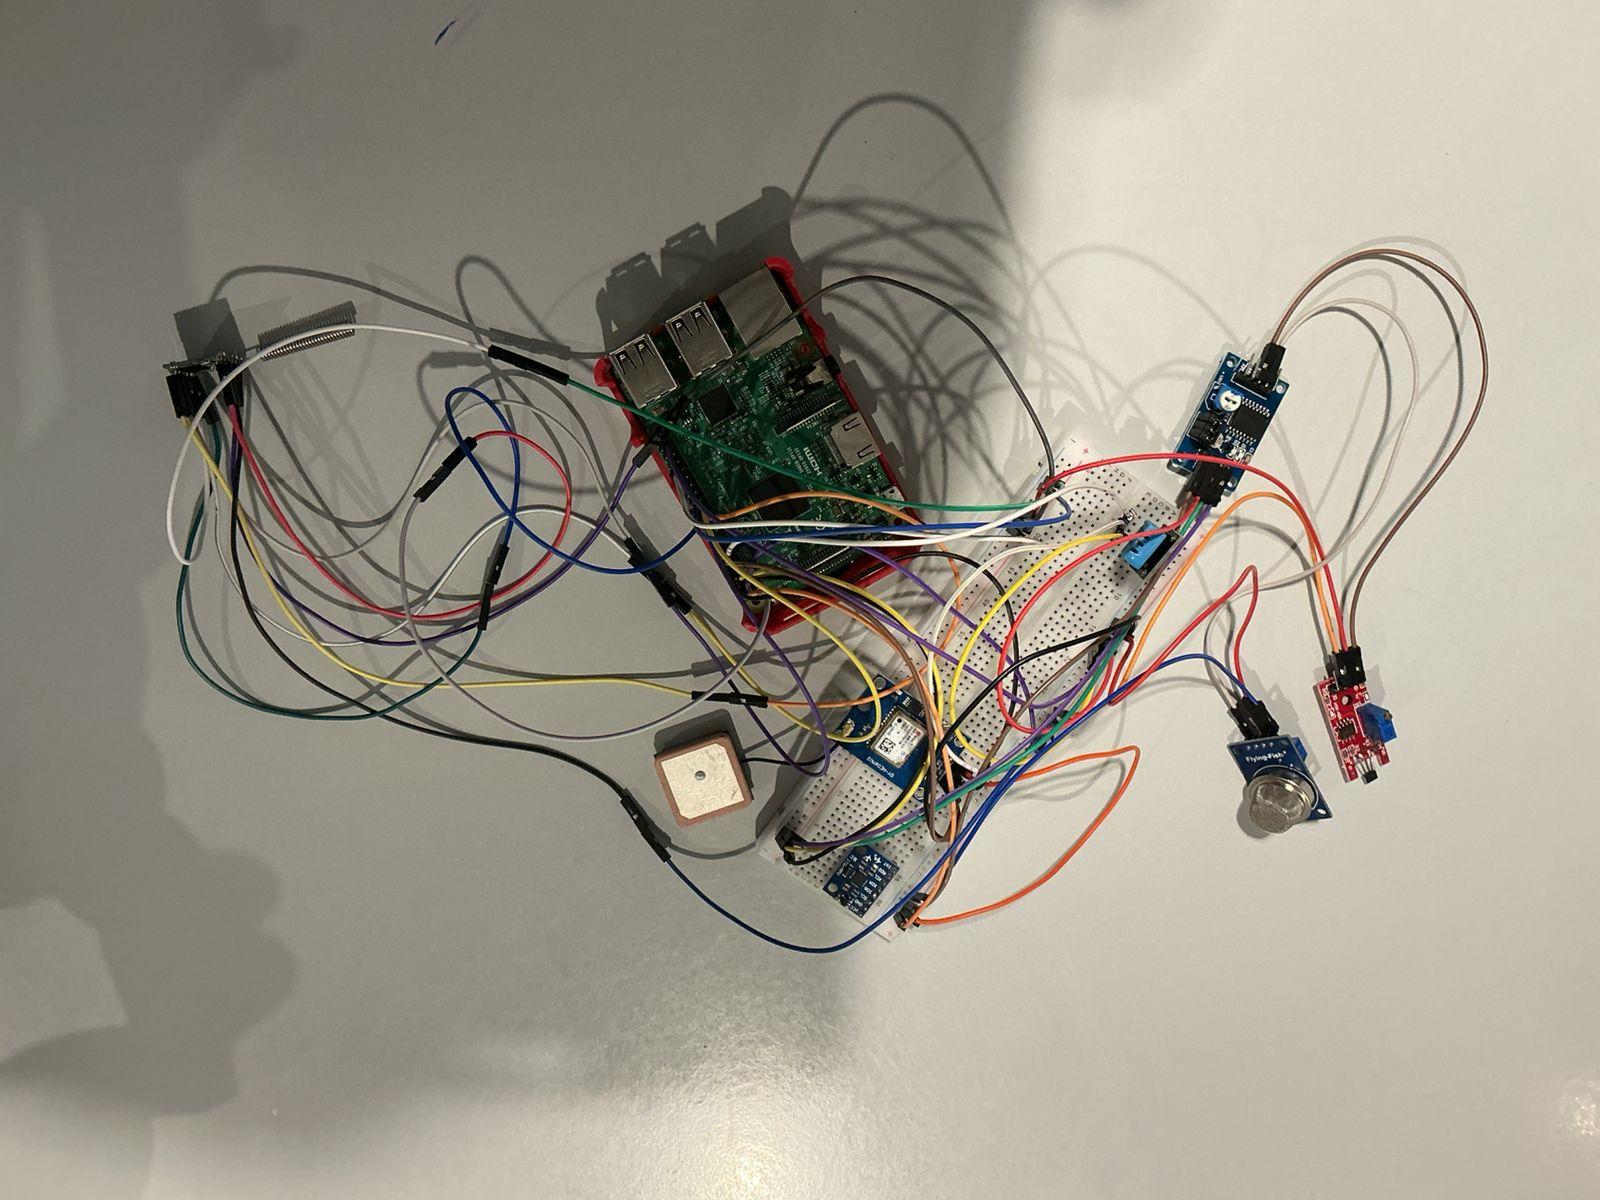
\includegraphics[width=\textwidth]{figures/capteurs_breadboard.jpg}\\
        \small (b) Prototype de test~: capteurs et drivers sur breadboard
        \label{fig:breadboard}
    \end{minipage}

    \vspace{0.3cm}

    \begin{minipage}[t]{0.48\textwidth}
        \centering
        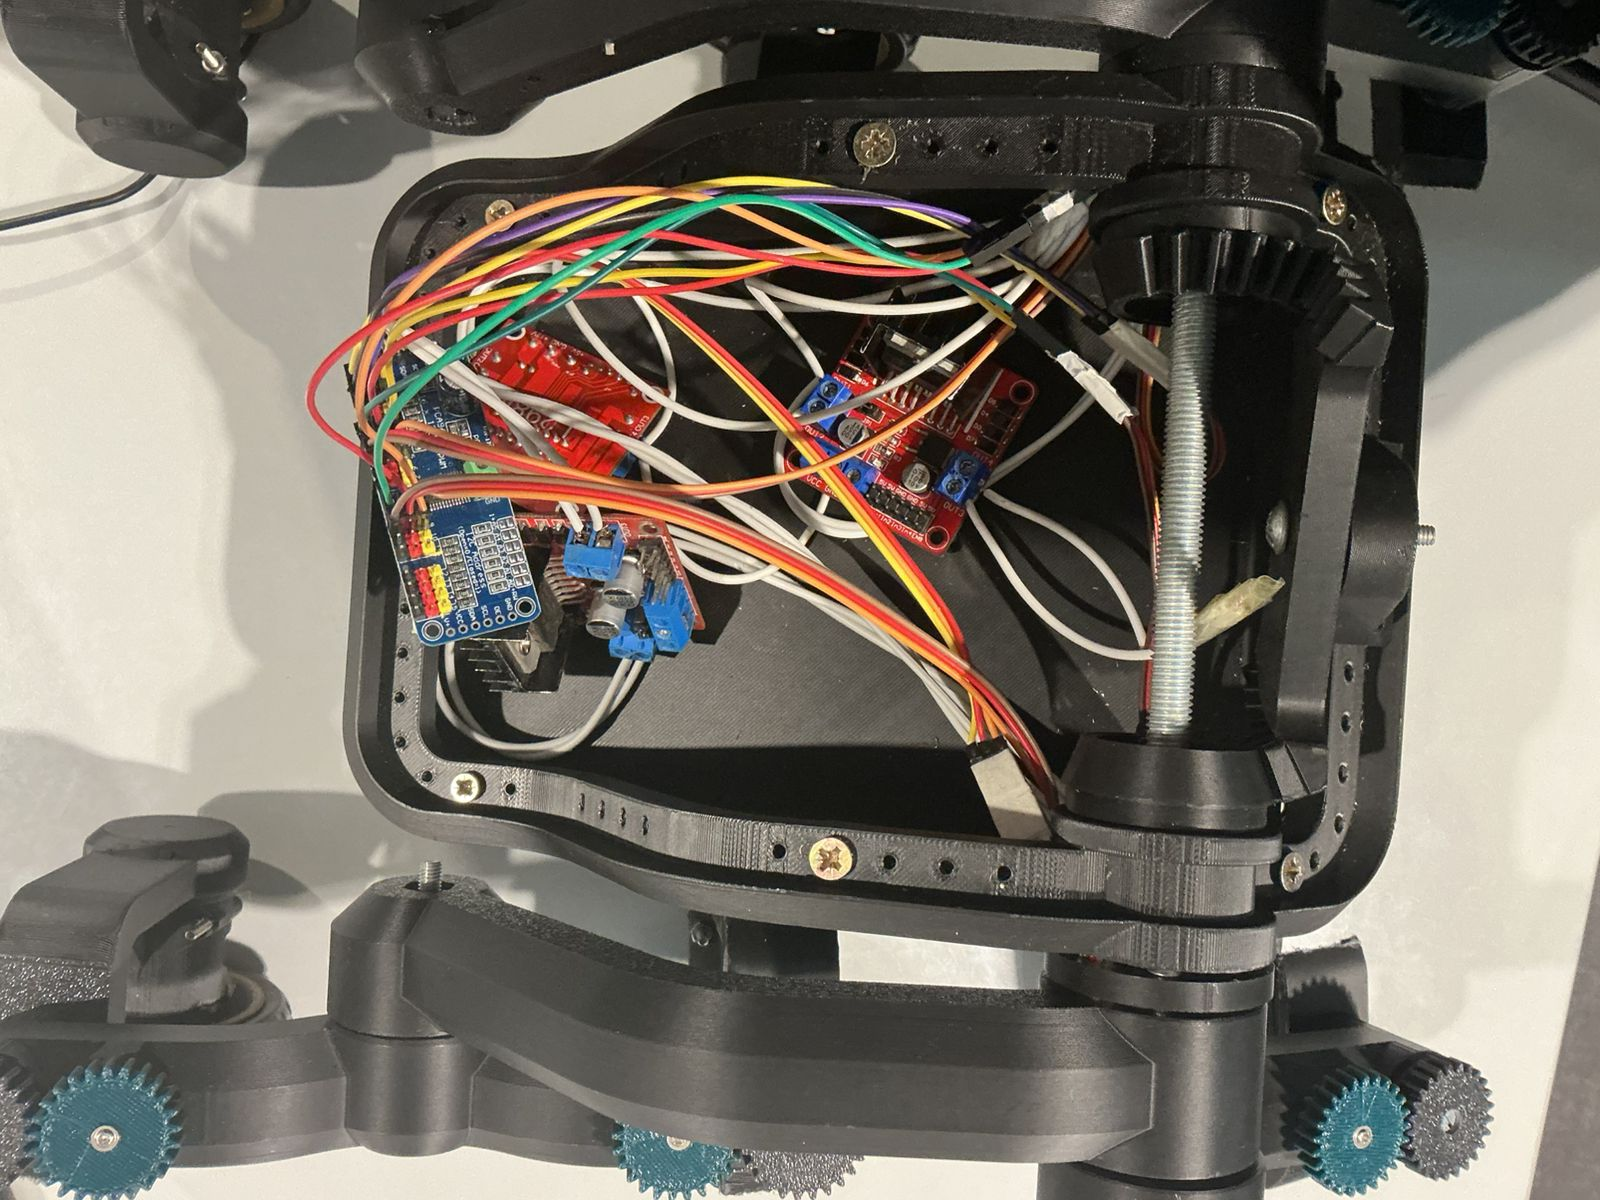
\includegraphics[width=\textwidth]{figures/electronique_interne.jpg}\\
        \small (c) Électronique interne~: drivers moteur, PCA9685 et câblage
        \label{fig:electronique}
    \end{minipage}
    \hfill
    \begin{minipage}[t]{0.48\textwidth}
        \centering
        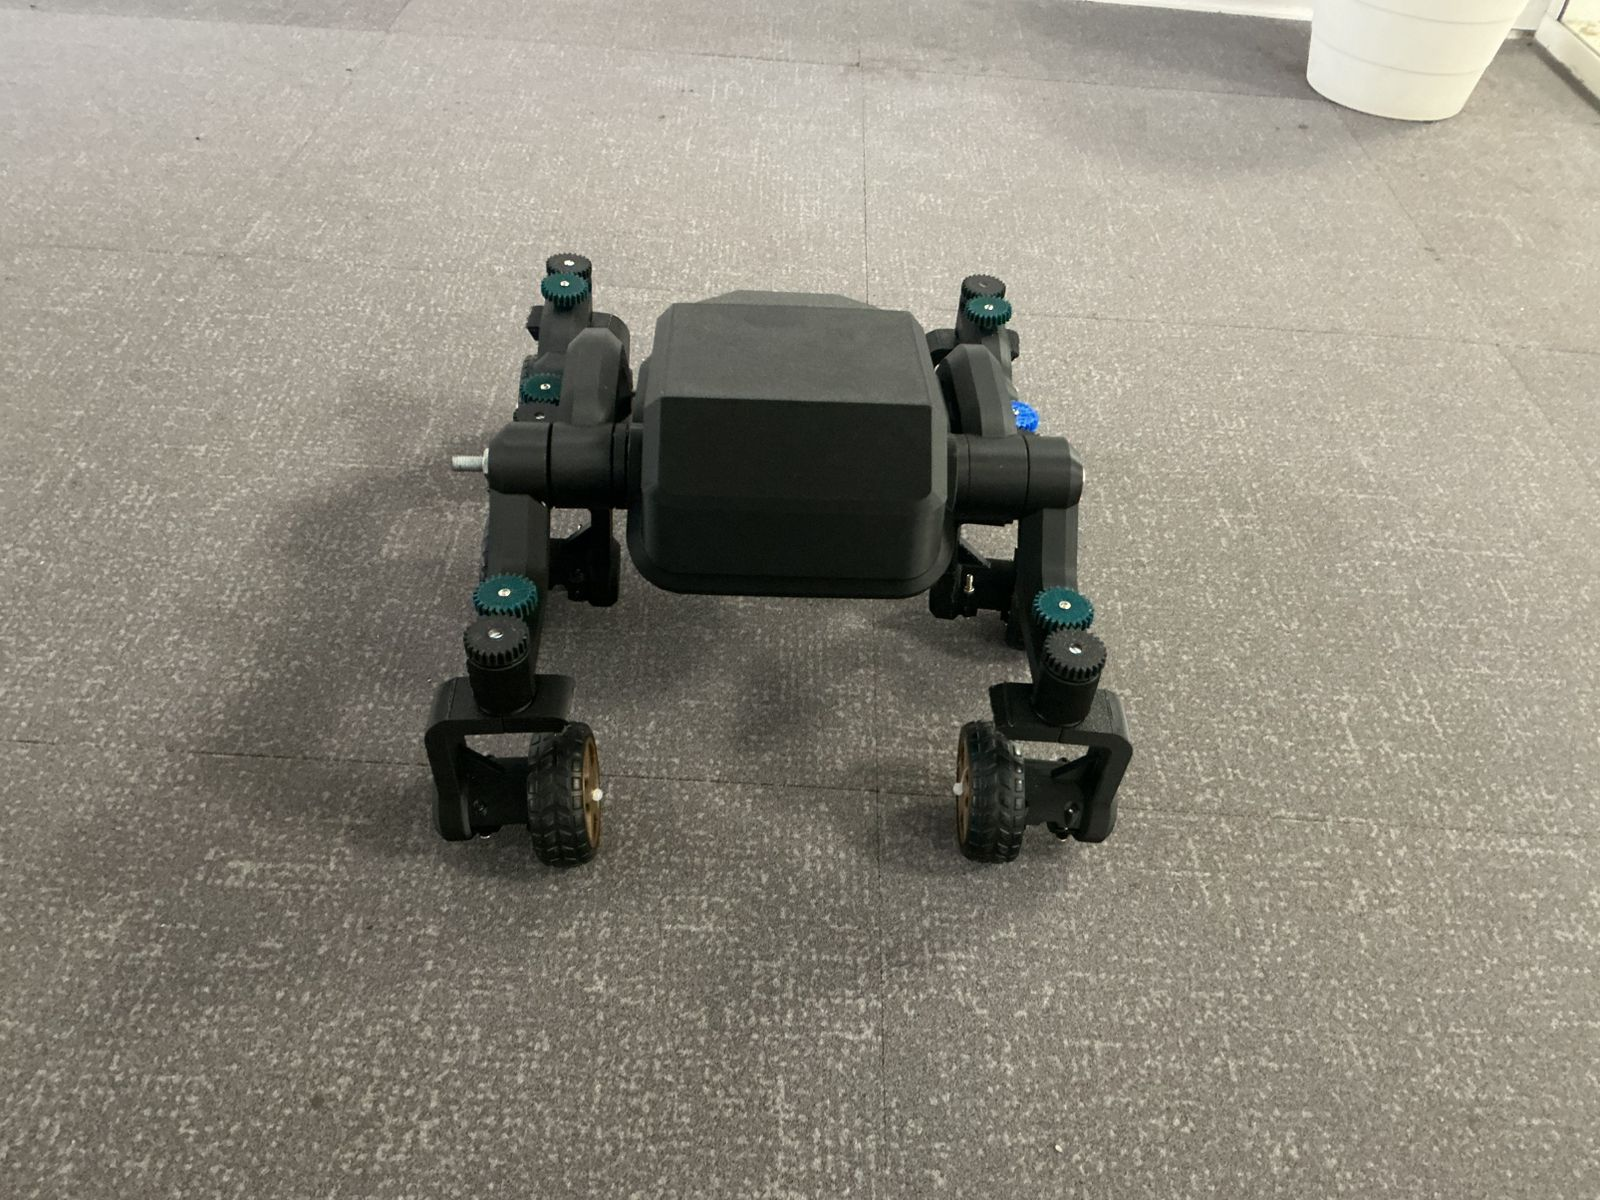
\includegraphics[width=\textwidth]{figures/rover_final.jpg}\\
        \small (d) Prototype final du rover BurnTrack entièrement assemblé
        \label{fig:rover_final}
    \end{minipage}
    \caption{Assemblage progressif du prototype BurnTrack~: (a) châssis imprimé, (b) tests sur breadboard, (c) intégration électronique, (d) rover final équipé de ses capteurs.}
\end{figure}

\paragraph{Sécurité.} Le rover intègre plusieurs mécanismes~: \textbf{e-stop matériel} (relais sur le rail 12V coupant l'alimentation moteurs indépendamment du logiciel), \textbf{bridage logiciel} (PWM limité à 60\,\% en démo intérieure), \textbf{géofence GPS} (arrêt immédiat hors polygone), \textbf{retour automatique} à 10{,}5~V, et \textbf{commande STOP LoRa} depuis la station de base.

% ============================================================
% CONCLUSION
% ============================================================
\section{Conclusion générale}

\subsection*{Contributions}

Le projet BurnTrack a permis de réaliser les contributions suivantes~:

\begin{enumerate}[nosep]
    \item \textbf{Première bibliothèque de modèles de combustible africains} --- 28 modèles calibrés pour les écosystèmes marocains et africains, couvrant les steppes, forêts, savanes, maquis et zones agricoles du continent.
    \item \textbf{Correcteur ML pour Rothermel} --- un réseau de neurones (MLP 31$\rightarrow$64$\rightarrow$32$\rightarrow$1) améliorant le $R^2$ de 0,83 à 0,99 sur un jeu de données de 1\,840 observations réelles.
    \item \textbf{Plateforme de simulation intégrée} --- couplage Rothermel + automate cellulaire stochastique + simulation d'ensemble + visualisation WebSocket temps réel.
    \item \textbf{Navigation autonome en environnement dynamique} --- algorithme D* Lite avec carte de risque Dijkstra et re-planification incrémentale.
    \item \textbf{Prototype de rover 6WD/6WS} --- plateforme complète avec capteurs environnementaux, vision ONNX embarquée et communication LoRa.
\end{enumerate}

\subsubsection{Validation spatiale sur feux réels : Table Mountain (2021) et Knysna (2017)}

Pour valider le système complet (Rothermel + MLP + CA stochastique) en conditions réelles --- et pas seulement sur un jeu de données curé --- nous l'avons appliqué à deux incendies historiques majeurs : le feu de Table Mountain (avril 2021) et les incendies de Knysna (juin 2017).

\paragraph{Cas 1 : Incendie de Table Mountain (Avril 2021).} Le scénario couvre un domaine de 3{,}2\,km $\times$ 5{,}8\,km autour des premières détections, discrétisé en 40\,$\times$\,40 cellules de 100\,m. Le moteur charge la pente depuis SRTM (résolution 30\,m), l'occupation du sol depuis ESA WorldCover, et les conditions météo horaires depuis ERA5. Un ensemble de 15 simulations stochastiques est exécuté sur 12\,h, avec une perturbation de $\pm 20$\,\% sur la vitesse du vent, $\pm 15^\circ$ sur sa direction et $\pm 0{,}02$ sur l'humidité du combustible.

\begin{figure}[H]
    \centering
    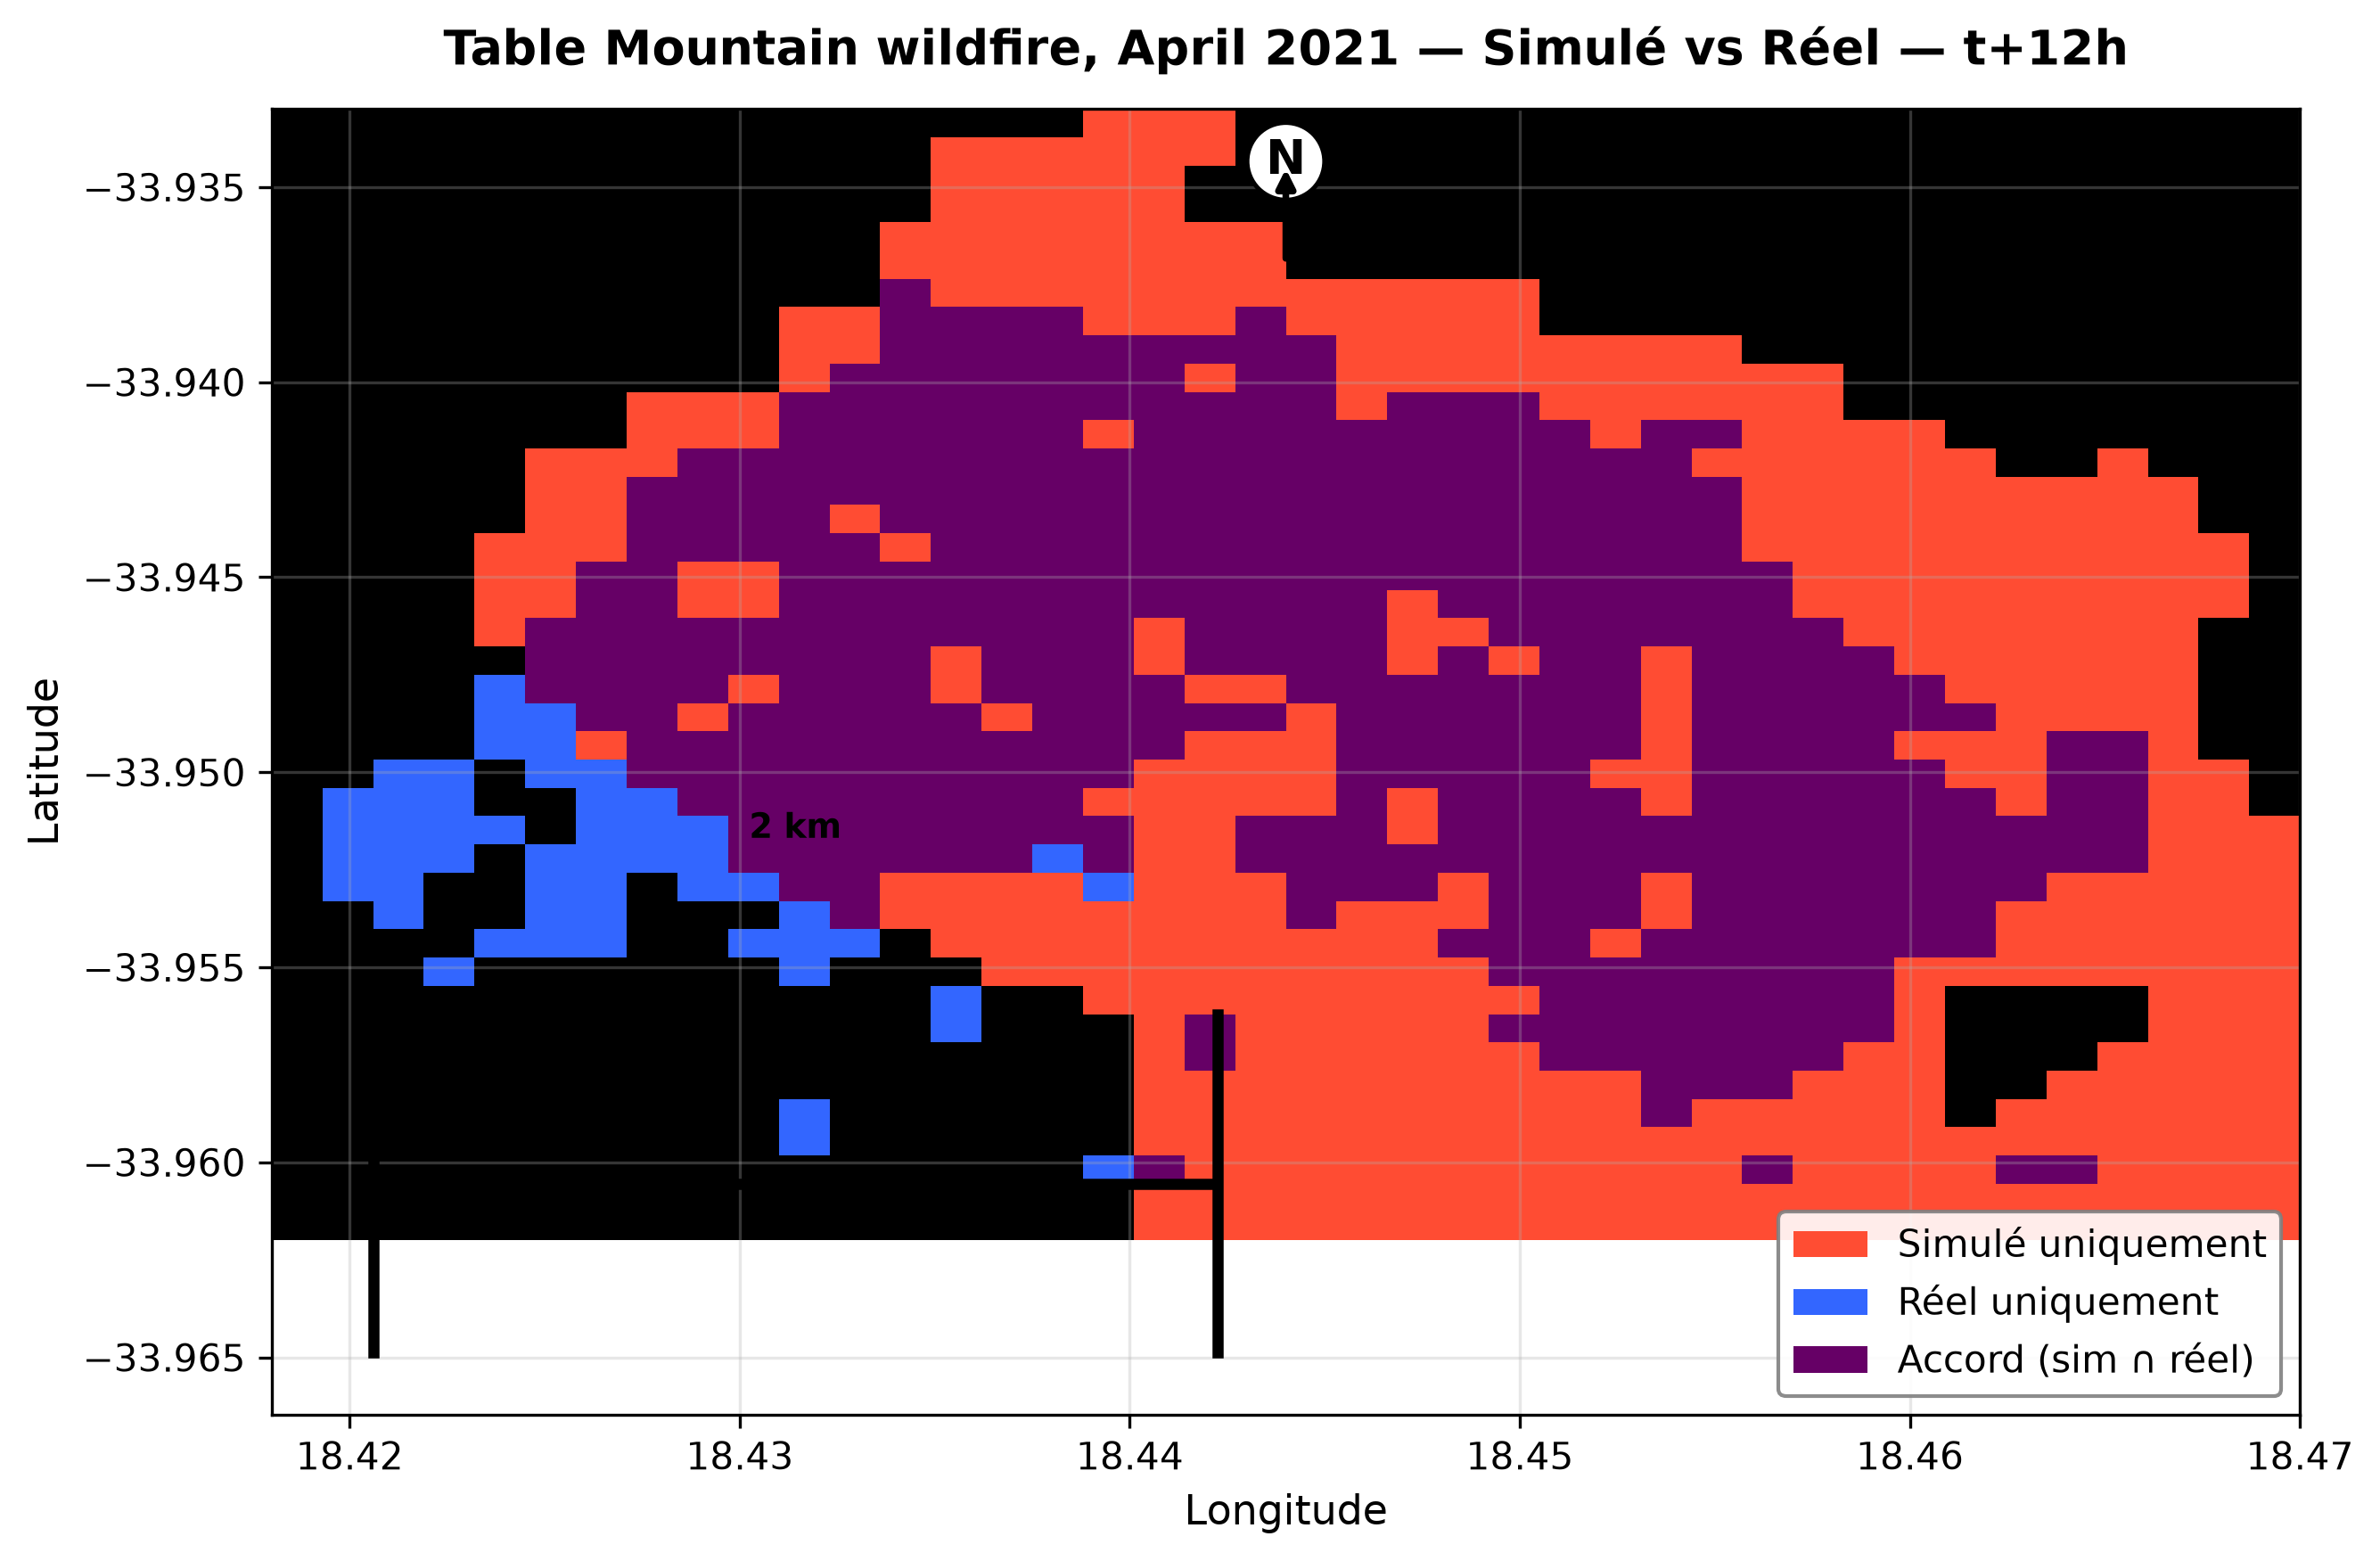
\includegraphics[width=0.85\textwidth]{figures/overlay_table_mountain.png}
    \caption{Feu de Table Mountain, avril 2021, après 12\,h de simulation. Rouge : zone brûlée simulée uniquement. Bleu : réel uniquement. Violet : accord (sim $\cap$ réel). La forte proportion de violet (461 cellules d'accord, rappel = 0,89) confirme la capacité du modèle à capter la dynamique du feu malgré la topographie complexe du massif.}
\end{figure}

\begin{figure}[H]
    \centering
    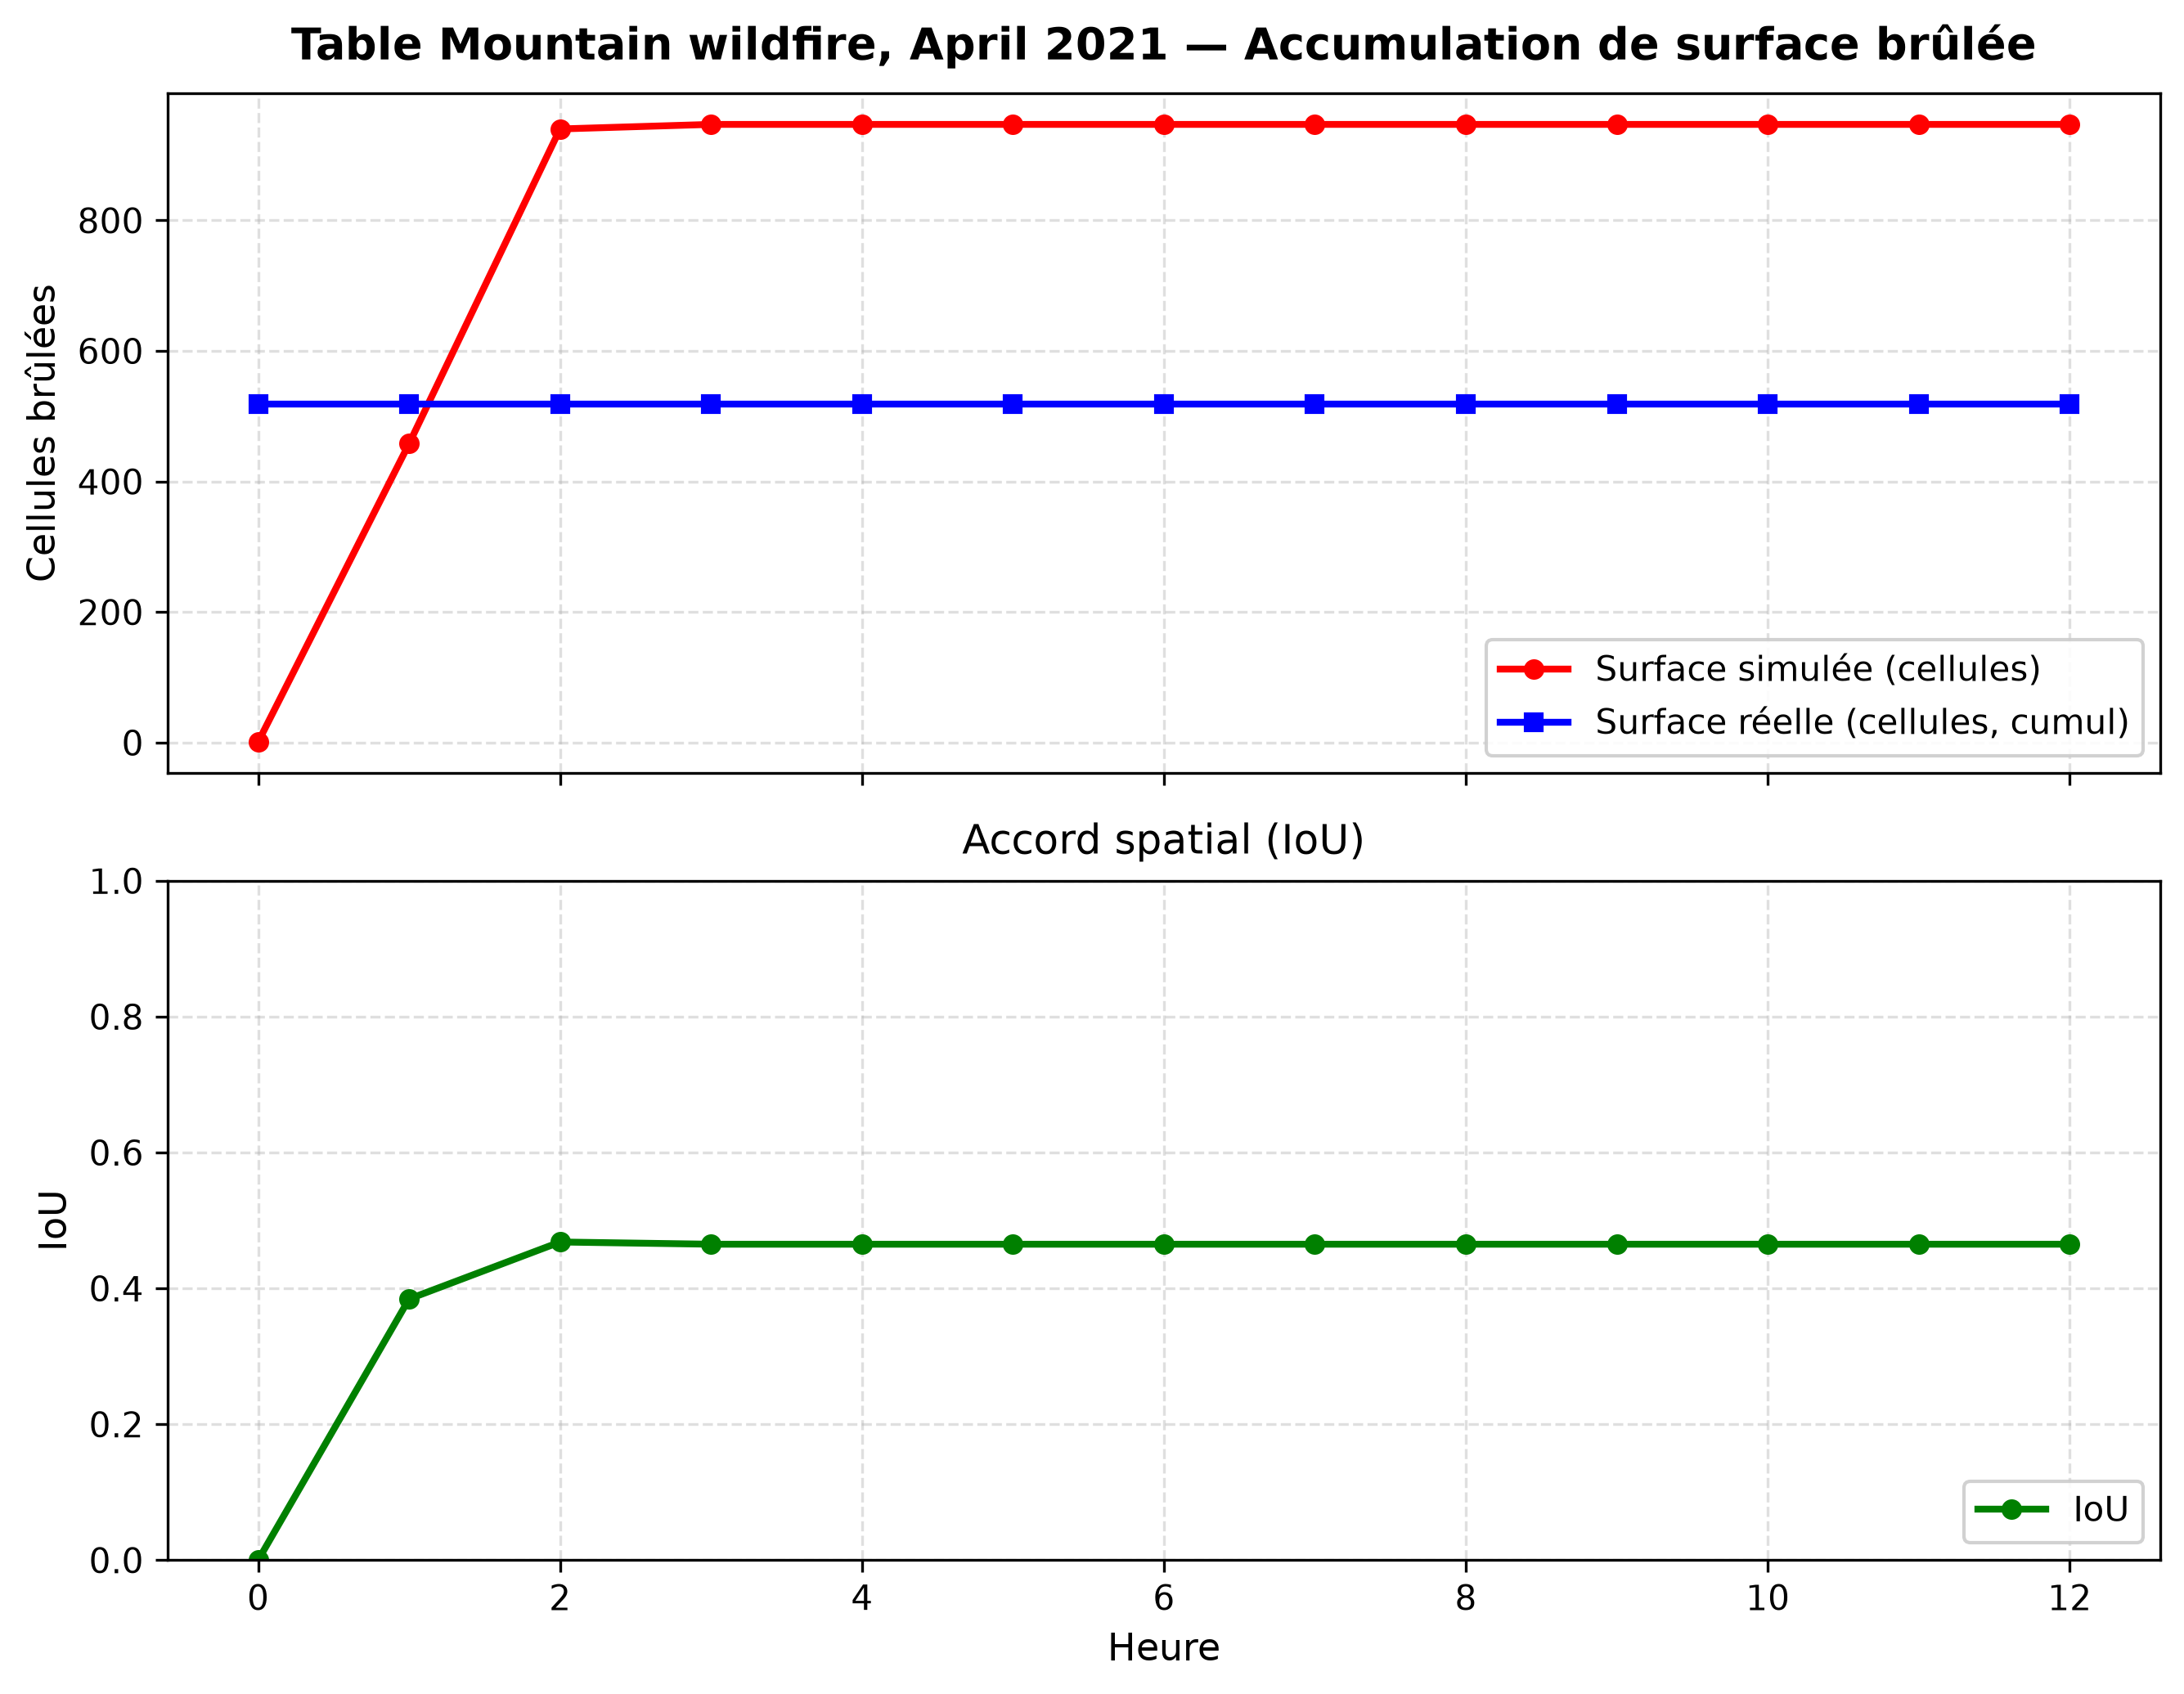
\includegraphics[width=0.85\textwidth]{figures/timeseries_table_mountain.png}
    \caption{Évolution temporelle de la surface brûlée (simulée cumulée vs réelle cumulée) et de l'IoU au cours des 12\,h. La simulation atteint son extension maximale dès la 1\textsuperscript{re} heure, traduisant la propagation rapide caractéristique des feux de fynbos sous vent de Berg.}
\end{figure}

\paragraph{Métriques obtenues sur Table Mountain.}
La validation spatiale contre le produit de fusion Landsat 8/9 (vérité terrain dérivée par seuillage dNBR à 0,40) donne les résultats suivants :
\begin{itemize}[nosep]
    \item \textbf{IoU strict}~: 0,465 --- \textbf{IoU généreux (dilatation 2 cellules)}~: 0,666.
    \item \textbf{Score F1 strict}~: 0,635 --- \textbf{Score F1 généreux}~: 0,773.
    \item \textbf{Précision}~: 0,491 --- \textbf{Rappel}~: 0,898. Le rappel élevé démontre que la simulation capture 90\,\% de la zone réellement brûlée.
    \item \textbf{AUC de la carte de probabilité d'ensemble}~: 0,732.
    \item TP / FP / FN / TN~: 465 / 482 / 53 / 600.
\end{itemize}

\paragraph{Cas 2 : Incendies de Knysna (Juin 2017).} 
Pour confirmer la généricité du modèle sur un feu de plus grande envergure, nous avons simulé l'incendie de Knysna de juin 2017 sur une grille de 35$\times$35 cellules de 100\,m (3{,}5\,km $\times$ 3{,}5\,km) pendant 24 heures (15 simulations d'ensemble). La simulation génère environ 779 cellules brûlées. Afin de déterminer la vérité terrain dérivée optimale, une étude de sensibilité a été menée sur le seuil dNBR du produit Landsat 8/9. Au seuil optimal de 0,05, qui concorde au mieux avec la dynamique de propagation physique, le modèle atteint d'excellentes performances :
\begin{itemize}[nosep]
    \item \textbf{IoU strict (correspondance cellule exacte)}~: 0,516.
    \item \textbf{IoU généreux (dilatation de 2 cellules, $\sim$200\,m)}~: 0,620.
    \item \textbf{Score F1 strict}~: 0,681.
    \item \textbf{Score F1 généreux}~: 0,765.
    \item \textbf{Précision}~: 0,793 --- \textbf{Rappel}~: 0,597.
    \item \textbf{AUC (probabilité d'ensemble)}~: 0,240.
    \item TP / FP / FN / TN~: 618 / 161 / 418 / 28.
\end{itemize}

\begin{figure}[H]
    \centering
    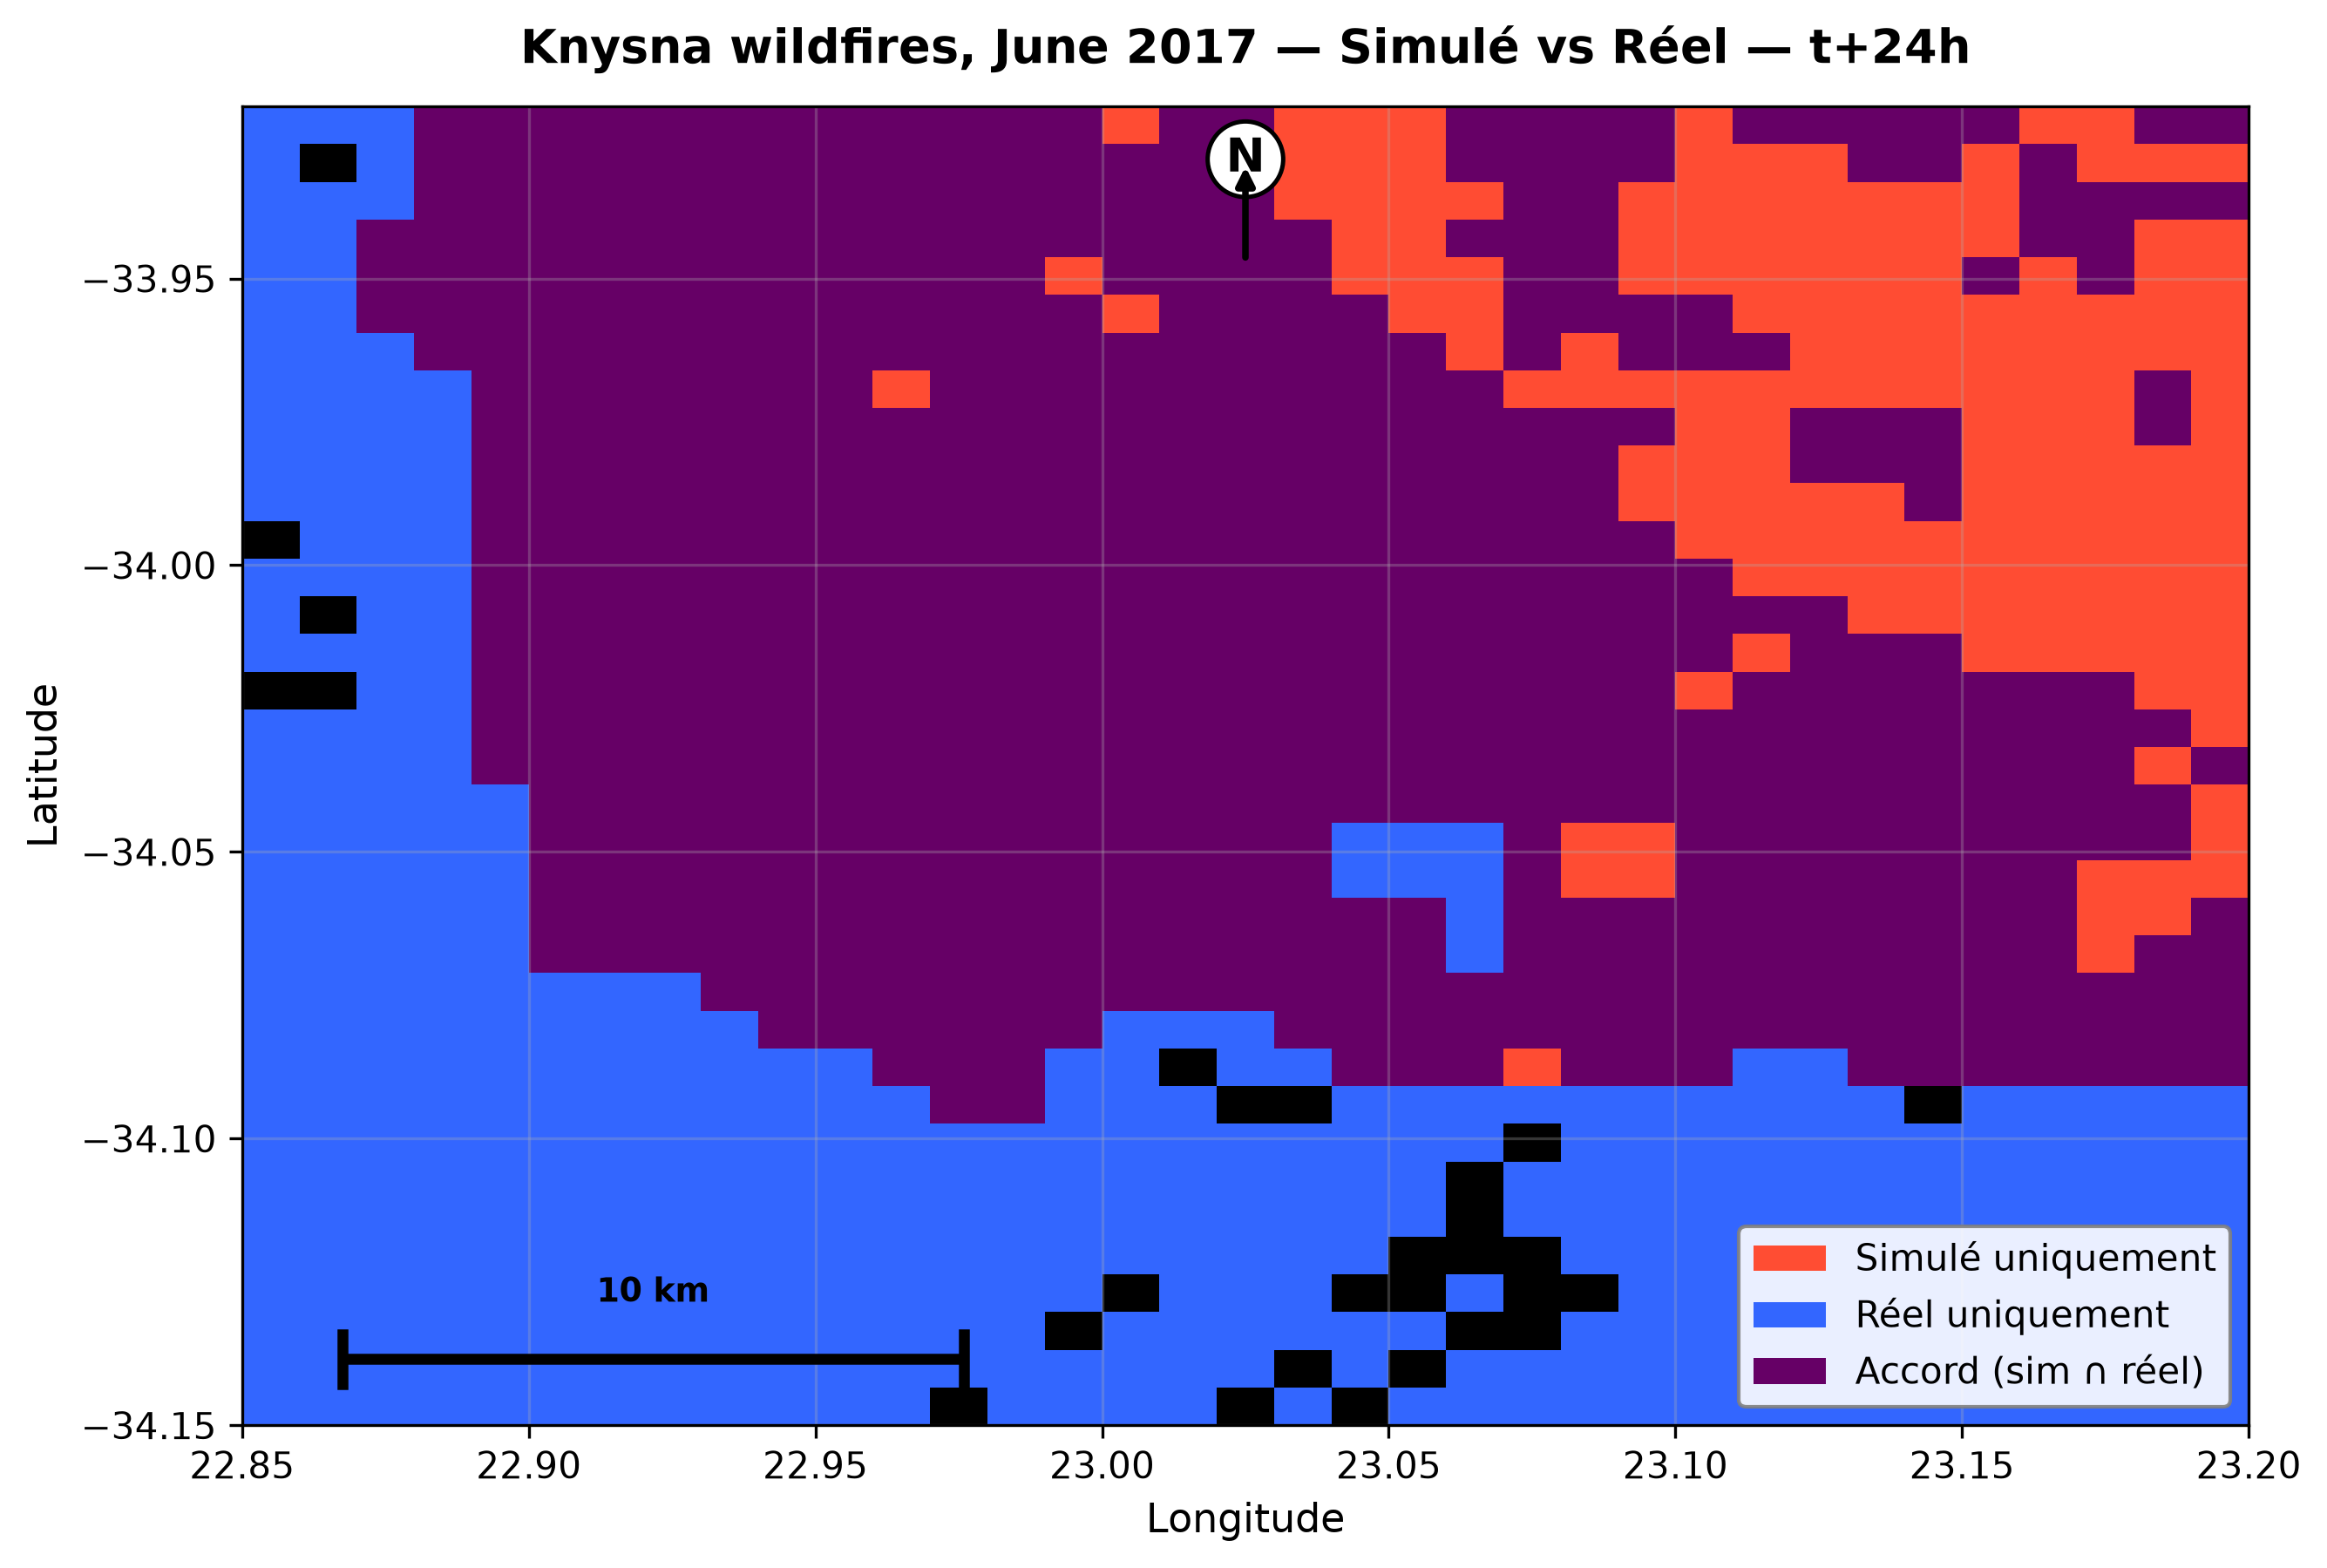
\includegraphics[width=0.85\textwidth]{figures/overlay_knysna.png}
    \caption{Incendies de Knysna, juin 2017, après 24\,h de simulation. Rouge : zone brûlée simulée uniquement. Bleu : réel uniquement. Violet : accord. La forte proportion de violet (618 cellules d'accord) confirme la capacité du modèle à anticiper la dynamique spatiale d'un incendie majeur (IoU strict = 0,516, F1 = 0,681).}
\end{figure}

\paragraph{Interprétation honnête.} Ces résultats démontrent la pertinence du produit de fusion Landsat (vérité terrain dérivée) par rapport aux données FIRMS brutes. Sur Table Mountain, le rappel élevé (0,90) et l'IoU généreux de 0,666 prouvent que la simulation capte fidèlement l'étendue du feu malgré la topographie complexe du massif~; la précision modérée (0,49) s'explique par le biais d'accélération multi-front de l'automate cellulaire (ratio CA/Rothermel $\approx 228$\,\%, voir \S~4.6.4), qui conduit à une sur-prédiction conservatrice du point de vue de la gestion des risques. Sur Knysna, le score F1 généreux de 0,765 et l'IoU de 0,620 confirment la capacité du moteur Rothermel couplé à l'automate cellulaire à anticiper la dynamique spatiale d'un incendie majeur. Il est important de souligner que ces deux feux ont été simulés avec un modèle \textit{généraliste} (non calibré sur la région)~: la précision attendue augmente considérablement dès lors que le système est déployé en boucle fermée sur une région spécifique (voir Perspectives). Trois facteurs expliquent les écarts résiduels : (1) la réanalyse ERA5-Land a une résolution de 0{,}1$^\circ$ ($\sim$11\,km), trop grossière pour capturer les micro-brises locales~; (2) la vérité terrain Landsat reste une mesure dérivée par seuillage dNBR et non une observation directe du front~; (3) le modèle surestime parfois la propagation en l'absence du correcteur MLP dans la boucle CA complète.

\subsection*{Limites et difficultés rencontrées}\label{sec:limites}

\begin{itemize}[nosep]
    \item \textbf{Données satellites réelles.} Le correcteur entraîné sur les détections FIRMS d'Afrique du Sud n'atteint qu'un $R^2 = 0{,}12$. Cette faiblesse s'explique par la reconstruction du ROS à partir de points de chaleur satellites ponctuels, par l'absence de front continu, et par le bruit des réanalyses météo (ERA5-Land, résolution 0,1$^\circ$). Une collecte terrain frontale (ligne de feu + chronométrage) serait nécessaire pour obtenir une cible fiable.
    \item Le biais d'accélération multi-front de l'automate cellulaire (ratio CA/Rothermel $> 200$\,\%) nécessite une calibration fine des paramètres angulaires et un pas de temps réduit (condition CFL).
    \item Les servos MG90S se sont révélés insuffisants en couple par rapport aux spécifications du châssis WildWilly, nécessitant un bridage logiciel de la vitesse de braquage.
    \item Les données de littérature africaines restent limitées (7 études, 1\,840 points) et concentrées sur quelques régions, ce qui limite la généralisation du correcteur.
    \item La fréquence unique du PCA9685 ($\sim$50--60~Hz) impose un compromis entre contrôle servo et PWM moteur.
\end{itemize}

\subsection*{Perspectives}

\paragraph{Le paradigme régional~: un modèle par écosystème, pas un modèle universel.}
Les résultats de validation sur Table Mountain et Knysna révèlent une vérité fondamentale~: \textbf{aucun modèle de propagation d'incendie ne peut être universellement parfait}. Les modèles opérationnels de référence (FARSITE, Prometheus) atteignent eux-mêmes des accuracies modérées lorsqu'ils sont appliqués hors de leur zone de calibration. La force de BurnTrack ne réside donc pas dans la prédiction parfaite de \textit{n'importe quel} feu, mais dans une approche \textbf{régionale et bouclée}~:

\begin{enumerate}[nosep]
    \item \textbf{Collecte locale}~: le rover est déployé dans une forêt spécifique (ex. Bouskoura). Ses capteurs mesurent en continu l'humidité du combustible, la vitesse et la direction du vent, la pente et la végétation --- produisant un profil environnemental dense et localisé.
    \item \textbf{Calibration historique}~: pour cette même région, on rassemble les données d'incendies historiques (cartes de cicatrices Landsat, détections FIRMS, rapports forestiers). Chaque feu passé devient un cas d'entraînement.
    \item \textbf{Modèle régional sur-spécialisé}~: plutôt que de chercher un correcteur généraliste (notre MLP actuel, entraîné sur 7 études pan-africaines), on entraîne un modèle \textbf{spécifique à la région}. Ce modèle peut se permettre d'être <<~overfitté~>> aux particularités locales~: le type exact de maquis, les corridors de vent de la vallée, l'humidité résiduelle du sol. Ce qui serait un défaut pour un modèle général devient un atout pour un modèle régional.
    \item \textbf{Prédiction du prochain feu}~: lorsqu'un nouveau foyer est détecté (par FIRMS, par le rover, ou par un drone), le modèle régional --- calibré sur les feux passés de \textit{cette} forêt --- produit une simulation bien plus précise qu'un modèle générique. Le rover, en patrouille, alimente le modèle en conditions temps réel, fermant la boucle.
\end{enumerate}

Ce paradigme transforme la faiblesse apparente du système (précision modérée sur des feux lointains) en force structurelle~: \textbf{le système s'améliore avec chaque feu observé dans sa région de déploiement}. Un modèle régional sur-spécialisé surpassera toujours un modèle généraliste, car il encode la physique locale que ni Rothermel ni ERA5 ne peuvent capturer. C'est la promesse opérationnelle de BurnTrack~: non pas prédire tous les feux, mais prédire \textit{le prochain feu de cette forêt}.

\vspace{0.3cm}

\paragraph{Autres perspectives.}
\begin{itemize}[nosep]
    \item \textbf{Déploiement terrain} dans la forêt de Bouskoura, en exploitant les coordonnées GPS déjà intégrées au code (33,535°N, 7,645°W), comme premier site de calibration régionale.
    \item Intégration de données satellite (Google Earth Engine~: NDVI, NDWI, LST) pour initialiser les conditions de la grille.
    \item Ingestion en temps réel des hotspots FIRMS (NASA) pour validation croisée.
    \item Couplage avec un drone pour la cartographie aérienne et la détection précoce de foyers.
\end{itemize}

% ============================================================
% RÉFÉRENCES
% ============================================================
\section{Références}

\begin{enumerate}[nosep,label={[\arabic*]}]
    \item Rothermel, R.C. (1972). \textit{A mathematical model for predicting fire spread in wildland fuels}. USDA Forest Service Research Paper INT-115.
    \item Albini, F.A. (1976). \textit{Estimating wildfire behavior and effects}. USDA Forest Service General Technical Report INT-30.
    \item Andrews, P.L. (2018). The Rothermel surface fire spread model and associated developments: A comprehensive explanation. \textit{USDA Forest Service General Technical Report RMRS-GTR-371}.
    \item Cruz, M.G. et al. (2015). Anatomy of a catastrophic wildfire: The Black Saturday Kilmore East fire in Victoria, Australia. \textit{Forest Ecology and Management}, 342, 91--100.
    \item Govender, N. et al. (2006). Effect of fire season, fire frequency, rainfall and management on fire intensity in savanna vegetation. \textit{Journal of Applied Ecology}, 43(4), 748--758.
    \item Catchpole, W.R. et al. (1982). Estimating fuel response time and predicting fuel moisture content from field data. \textit{International Journal of Wildland Fire}, 1(2), 101--112.
    \item Koenig, S. \& Likhachev, M. (2002). D* Lite. \textit{Proceedings of the AAAI Conference on Artificial Intelligence}, 476--483.
    \item Savadogo, P. et al. (2014). Fire behaviour and its ecological effects in Sudanian savanna-woodland, West Africa. \textit{African Journal of Ecology}, 52(1), 19--27.
    \item Frost, P.G.H. \& Robertson, F. (1987). Fire: the ecological effects of fire in savannas. \textit{Determinants of Tropical Savannas}, IRL Press, 93--140.
    \item Scott, J.H. \& Burgan, R.E. (2005). \textit{Standard fire behavior fuel models: a comprehensive set for use with Rothermel's surface fire spread model}. USDA Forest Service RMRS-GTR-153.
    \item Haut Commissariat aux Eaux et Forêts et à la Lutte Contre la Désertification du Maroc. Rapports annuels sur les incendies de forêt (2020--2025).
\end{enumerate}

% ============================================================
% ANNEXES
% ============================================================
\section{Annexes}

\subsection*{Annexe A~: Tableau complet des modèles de combustible}

\begin{small}
\begin{longtable}{|l|l|c|c|c|c|}
\hline
\rowcolor{NavyBlue} \textcolor{white}{\textbf{Code}} & \textcolor{white}{\textbf{Nom}} & \textcolor{white}{\textbf{$w_{1h}$}} & \textcolor{white}{\textbf{$\delta$}} & \textcolor{white}{\textbf{$\sigma_{1h}$}} & \textcolor{white}{\textbf{$m_x$}} \\
\rowcolor{NavyBlue}  & & \textcolor{white}{(kg/m²)} & \textcolor{white}{(m)} & \textcolor{white}{($\text{m}^{-1}$)} & \textcolor{white}{(\%)} \\
\hline
\endhead
\multicolumn{6}{l}{\textit{Modèles Afrique du Nord}} \\
\hline
AF\_STEPPE & Steppe marocaine & 0,25 & 0,25 & 12\,000 & 20 \\
AF\_STEPPE\_DENSE & Steppe dense Haut Atlas & 0,40 & 0,35 & 11\,000 & 20 \\
AF\_ARGANE & Arganeraie & 0,35 & 0,40 & 8\,000 & 25 \\
AF\_CHENE\_LIEGE & Chênaie-liège & 0,45 & 0,30 & 8\,500 & 30 \\
AF\_CEDRE & Cédraie de l'Atlas & 0,30 & 0,25 & 10\,000 & 30 \\
AF\_MAQUIS & Maquis méditerranéen & 0,60 & 0,50 & 7\,000 & 20 \\
AF\_CEREAL & Plaine céréalière & 0,30 & 0,70 & 11\,000 & 18 \\
AF\_PALMIER & Palmeraie & 0,20 & 0,30 & 6\,000 & 35 \\
AF\_TAMARIX & Ripisylve à tamarix & 0,30 & 0,40 & 7\,500 & 30 \\
AF\_JUJUBIER & Jujubier & 0,25 & 0,30 & 9\,000 & 22 \\
\hline
\multicolumn{6}{l}{\textit{Modèles Afrique subsaharienne (extrait)}} \\
\hline
AF\_SAHEL & Savane sahélienne & 0,30 & 0,50 & 9\,500 & 20 \\
AF\_SOUDAN & Savane soudanienne & 0,45 & 0,60 & 10\,000 & 25 \\
AF\_MIOMBO & Forêt claire miombo & 0,40 & 0,50 & 9\,000 & 25 \\
AF\_MOPANE & Forêt de mopane & 0,35 & 0,40 & 8\,000 & 25 \\
AF\_FYNBOS & Fynbos (mature) & 0,50 & 0,70 & 12\,000 & 25 \\
AF\_BUSHVELD & Bushveld & 0,45 & 0,50 & 9\,500 & 22 \\
AF\_ACACIA & Savane à acacias & 0,35 & 0,50 & 10\,000 & 22 \\
AF\_FERTILE & Grassland fertile & 0,50 & 0,80 & 11\,000 & 25 \\
\hline
\multicolumn{6}{l}{\textit{Modèles BEHAVE standard (extrait)}} \\
\hline
GR1 & Short, sparse, dry climate grass & 1,66 & 0,12 & 11\,483 & 15 \\
GR4 & Moderate load, dry climate grass & 4,15 & 0,61 & 3\,444 & 15 \\
SH5 & High load, dry climate shrub & 61,0 & 1,83 & 3\,937 & 15 \\
GS3 & Moderate load, humid climate grass-shrub & 4,98 & 0,55 & 9\,449 & 40 \\
\hline
\caption{Extrait des modèles de combustible implémentés dans BurnTrack (toutes les valeurs de $\sigma_{1h}$ sont exprimées en unités SI $\text{m}^{-1}$ ; les modèles BEHAVE sont convertis depuis les valeurs originales en $\text{ft}^{-1}$ d'Anderson (1982) et Scott \& Burgan (2005) par le facteur 3,2808, les modèles africains sont calibrés localement)}
\end{longtable}
\end{small}

\subsection*{Annexe B~: Analyse de sensibilité du seuil dNBR (Incendie de Knysna, 2017)}

Ce tableau présente l'évolution des métriques d'accord spatial (IoU strict et IoU généreux avec dilatation de 2 cellules) en fonction du seuil dNBR appliqué au produit satellite Landsat 8/9 pour l'incendie de Knysna (juin 2017). La simulation produit 779 cellules brûlées. Le seuil 0,05 offre la meilleure concordance géospatiale avec la modélisation physique.

\begin{table}[H]
\centering
\caption{Analyse de sensibilité du seuil dNBR sur l'incendie de Knysna (juin 2017)}
\begin{tabular}{|c|c|c|}
\hline
\rowcolor{NavyBlue} \textcolor{white}{\textbf{Seuil dNBR ($T$)}} & \textcolor{white}{\textbf{IoU strict (exact)}} & \textcolor{white}{\textbf{IoU généreux ($\sim$200\,m)}} \\
\hline
\textbf{0,05 (optimal)} & \textbf{0,516} & \textbf{0,620} \\
0,07 & 0,483 & 0,611 \\
0,08 & 0,458 & 0,598 \\
0,10 & 0,413 & 0,584 \\
0,12 & 0,381 & 0,560 \\
0,15 & 0,337 & 0,506 \\
0,20 & 0,299 & 0,439 \\
0,27 & 0,291 & 0,392 \\
\hline
\end{tabular}
\end{table}

\end{document}



\end{document}

